\documentclass{report}

\RequirePackage{units}
\usepackage{amsmath,amsfonts,amssymb,mathtools}
\usepackage[margin=1in]{geometry}
\usepackage{graphicx} 
\usepackage{float}
\usepackage{pgfplots}
\usepackage{pgfplotstable}
\usepackage{hyperref}
\pgfplotsset{width=10cm,compat=1.9}
\usepackage{fancyhdr} 
\usepackage{tikz}
\usepackage{setspace}
\usepackage{caption}
\usepackage{booktabs}
\usepackage{units}

\usetikzlibrary{shapes.geometric, arrows.meta, positioning, 3d,calc}
\usetikzlibrary{shapes.arrows}



\pagestyle{fancy}
\fancyhf{}
\renewcommand{\headrulewidth}{0pt} 
\renewcommand{\footrulewidth}{0pt} 


\fancyfoot[L]{
    Supervisor:\\
    Dr. Pantelis Sopasakis\\
    School of EEECS%
}

\begin{document}
\onehalfspacing

\begin{titlepage}
    \begin{center}
        
        \textbf{\Large Design and Implementation of a Loitering Controller for a
        Quadcopter using a GNSS, Barometer, and Time of Flight Sensor}\\
        \vspace{1.5cm} 
        
        \textit{\large Software \& Electronic Systems Engineering}\\
        \vspace{0.5cm} 
        Final Year Project 2023-2024\\
        \vspace{2cm} 
        
        \textbf{Peter Davidson}\\
        \vspace{0.5cm} 
        \today
        
        \vfill
        
    \end{center}
    \thispagestyle{fancy}
\end{titlepage}
 
\newpage
\pagestyle{plain}

\section*{Declaration of Integrity}
I affirm that I am familiar with and have adhered to the plagiarism policies of
Queen's University for this report, which is solely my own creation. This work
has not been presented for any other assessment, and there has been no
unauthorized collaboration. I certify that this report includes a comprehensive
bibliography formatted according to the prescribed standards, accurately cites
all secondary sources, and has been carefully reviewed to ensure compliance with
the aforementioned requirements.
\newpage

\section*{Acknowledgements}
I would like to thank Dr Pantelis Sopasakis and Mr Jamie Rainey for there
continuous support throughout this project. 

I would like to especially thank Dr Pantelis Sopasakis, invaluable technical
assistance when it came to designing control algorithms, without said support
the project would not have been completed.
\newpage

\section*{Original specification}
Over the last couple of years, the Autonomous Systems Lab has been working on
the development of bzzz – a radio-controlled quad-rotor (see
https://github.com/QUB-ASL/bzzz for details). The quadcopter can now be flown in
manual mode using a radio controller where the operator controls the total
thrust directly, and in altitude hold mode where the quadcopter maintains a
reference altitude. The next step is to make the quadcopter maintain a given
reference (x, y, z)-position and heading. This is known as loitering mode
operation. In this project, you will design and implement a loitering mode
control system for bzzz. The main methodological tools for this will be the
linear-quadratic regulator (LQR) and the Kalman filter. The estimation of the
position of the quadcopter can be done using a GPS module in combination with
other sensors (IMU and altimeter etc.).
\subsection*{Problem Statement}
Throughout this project I will be designing a loitering controller for a
quadcopter. The objective of this is to enhance the quadcopters' ability to
maintain a fixed position in space with high accuracy and minimal drift, this is
a challenge in both commercial and civilian quadcopter use.

Loitering technology in drones offers a range of benefits and applications.
Security and surveillance, where home/business owners can have real time
surveillance, programming a quadcopter to parole specific areas. As well as
aerial photography and video, for those interested in photography or vloging,
drones with loitering capabilities will allow for stable and high-quality aerial
shots allowing for anything from time laps videos to landscape shots.

During the development of this project, I will be researching and implementing
various concepts, these will vary from what sensors to get, control and
estimation theory (using LQR, Kalman filter), python software development, PCB
design and so on. I will elaborate more on these concepts below.

\subsection*{Abstract}
This project aims to enhance quadcopter navigation and stability through advanced sensor integration and control systems to achieve loitering control. Key objectives include; the parsing of GNSS data streams for latitude, longitude and altitude values, the parsing of barometer pressure readings and converting them into altitude values, design and implementation of a Kalman filter utilising sensor fusion for the Time of Flight, GNSS and barometer altitudes, the design of a PD controller for altitude hold and a PID controller for position hold, design of various different PCB's, 3D printed model designs. Finally, the completion of various hardware tasks around the quadcopter including building and soldering various components.

\newpage
\subsection*{Objectives}
\begin{enumerate}
    \item To design, implement and test a Kalman filter to estimate the (x, y,
    z)-	position and the heading of the quadcopter using information from the
    IMU, the altimeter, and a GPS module.
    \item To design, implement and test a control system for loitering.
    \item To perform certain hardware tasks (proper mounting and connection of
    the GPS module to the on-board Raspberry Pi)
    \item To perform experiments and record flight data
\end{enumerate}

\subsection*{Learning Outcomes}
Upon successful completion of this project, I should:
\begin{enumerate}
    \item Have mastered the theory of LQR and Kalman filtering.
    \item Understand how a GPS module works and be able to interface it.
    \item Be able to design a PCB.
    \item Have a solid understanding of the attitude and translational dynamics
    of a quadcopter.
    \item Be able to perform simulations of dynamical systems in Python.
    \item Be able to operate a quadcopter using an RC.
    \item Be able to integrate different systems involving hardware and software
    components.
    \item Be able to use git and GitHub (branches, pull requests, etc).
\end{enumerate}
This project will involve (25\%) control and estimation theory of the LQR and
the Kalman filter, (40\%) software development – primarily in Python, (10\%)
some hardware tasks including, but not limited to PCB design, (15\%)
collaborative development using git and GitHub.

\newpage
\tableofcontents
\newpage


\chapter{Introduction}
Throughout this project a loitering controller will be designed for the
Quadcopter using a GNSS module, time of flight and barometer sensors. The objective of this is to enhance the quadcopters' ability to maintain a fixed position in space with high accuracy and minimal drift, this is a challenge in both commercial and civilian quadcopter use.

Loitering technology in drones offers a range of benefits and applications.
Security and surveillance, where home/business owners can have real time
surveillance, programming a quadcopter to parole specific areas. As well as
aerial photography and videography, for those interested in photography or
vloging, drones with loitering capabilities will allow for stable and
high-quality aerial shots allowing for anything from time lapse videos to
landscape shots.

\section{Literature review}
This project will include the development of UAV (Unmanned Aerial
Vehicle) technology which will be capable of position hold whilst flying.
Throughout the development of this project control algorithms and prediction theory will hae to be researched and implemented.

UAV's as described above have many applications in both commercial and military
use. Commercial applications include photography and video
\cite{photographyAndVideo}, home surveillance and security \cite{security},
quadcopter light shows \cite{lightShow}, agriculture \cite{agricultural} and
construction \cite{construction}. Some military applications might include
disaster management \cite{disasterManagement}, surveillance \cite{surveillance},
search and rescue \cite{searchAndRescue}.

Due to UAV's wide range of adaptability and use cases it has been researched
extensively all around the world. In the study \cite{Widhianto2023Quadcopter}
the researchers delve into the specifics of using GPS for location control in
quadcopters. Primarily the study focuses on enhancing the accuracy of position
holding, they have done this by utilising a way-point system where the
quadcopter autonomously navigates through pre-determined points.

The testing which was completed evaluated the quadcopters data supply, GPS
sensors used as sensors to determine vehicle coordination points, the LiDAR
sensor Lite-V3 is used for measuring altitude. This senor is accurate up to \(\pm 2.5\)cm and can read up to 500 values per second, priced around £120.

The waypoints, which were separated into three points at a distance of ten
metres each to form a triangular angle; the flights are carried out at 3
waypoints, which are 10 metres each other at a height of five metres; the
flights was conducted in the Autonomous mode; the tests were conducted six
times. The flight path was from the home base to waypoint, to waypoint 2, to
waypoint 3, all points were 10m apart. The quadcopters system performance was
evaluated based on error values between the actual vehicle position and the
waypoints coordinates.

They concluded that between waypoint 1 and home the best result they were able
to get was 35.8475 cm. between waypoint 1 and 2 the result was 16.2083cm and
finally between waypoint 2 and 3 it was 110.2508cm.

Factors to consider for large errors between waypoints that cause the
Quadcopter's level of accuracy to not be good are wind speed and inaccurate
tuning of the PID controller they were using, this is most prevalent when
testing between waypoint 2 and 3. Overall, although there could be improvements,
I think the results were good especially in test 2 between waypoint 1 and 2 as
they were off by only 16cm.

Furthermore, within this paper there is no evidence of researchers utilising the Kalman filter for position estimation. This would be useful, as if satellite connections were to drop suddenly, the Kalman filter could provide a reliable alternative for estimating the quadcopter's position by fusing readings of the GPS and LiDAR sensors. The Kalman filter, known for its efficiency in dealing with uncertainty and noise in sensor data, could allow for continuous and accurate position tracking even in the absence of GPS signals. This redundancy is crucial for maintaining the stability and safety of the quadcopter during flight, especially in environments where GPS signals are obstructed or non-existent. Incorporating such a filter could significantly enhance the robustness of the control system against signal drop-out, making the quadcopter more reliable for critical applications where consistent positioning is paramount.

The paper presents a detailed study on using GPS technology for the development
of an autonomous UAV quadcopter. The GPS module plays a crucial role in outdoor
navigation, particularly in altitude stabilization and trajectory mapping for
automated flights. The quadcopter uses GPS data for precise positioning and
executing flight paths, ensuring stability and accuracy in various outdoor
environments.

This study \cite{AkademiaBaru2016}  by P. Akademia Baru, S. Sabikan and S. Nawawi emphasizes the integration of GPS in
autonomous flight. The GPS facilitates precise positioning, which is paramount
for the quadcopter to execute its flight paths accurately. The described
precision is not just in horizontal positioning, but it also plays a big part in
maintaining a consistent altitude. The GPS data, combined with other on-board
sensors, forms a accurate and reliable solution for navigating complex
flightpaths in outdoor environments.

Moreover, the paper describes how GPS helps the quadcopter to map out its
trajectory, so that the UAV can follow. The waypoints, defined by GPS data, tell
the quadcopter which route to take, making it a desirable piece of equipment for
manned and unmanned coverage, surveillance, photography, surveying, weather
prediction, and search and rescue. GPS-enabled trajectory mapping enables the
quadcopter to fly through waypoints, correcting course upon arrival at each node
and in mid-course as environmental factors arise, such as wind.

PID control is an important part of quadcopter flight operations, especially in
stabilizing flight conditions. This control system adapts the quadcopter's
motors based on information provided by the sensors, helping to respond
accordingly to environmental changes and operator input. The paper describes the
use of PID control in the quadcopter system to ensure good stability in outdoor
environments. The PID parameters can be fine-tuned to optimize the response of
the quadcopter, increasing overall performance and reliability.

Through testing they also have taken into account the effects high vibrations on
the quadcopter and its effect on the accelerometer-based altitude and horizontal
position estimates to drift far off from reality. Thus, it will create problems
with altitude hold or loiter. To diminish the effects of vibrations they placed
the flight controller on an anti-vibration plate, this significantly reduced the
vibrations recorded on the IMU. Propeller and motor balancing, however, is also
critical for improved performance.

In the second experiment, mission planner software is used to create the flight
routes for the quadcopters in advance. they choose to use separate locations for
home and land. From WP1 to WP4, five randomly chosen waypoints were added, along
with an extra one-second delay. For the duration of the missions, the flight
altitude is fixed at 30 metres. The following are the speed settings for
waypoint navigation: 700 cm/s for linear speed, 200 cm/s for radius speed, 250
cm/s for speed up rate, 150 cm/s for speed down rate, and 1000 cm/s for loiter
speed. This flight mission is conducted six times.

I found that utilizing GPS, PID and compass technology they were able to make a
quadcopter that was able to follow pre-determined set waypoints with little to
no off set furthermore I cannot see any overshoot in and around the waypoints
meaning that there PID technology is optimized very well. Overall, this is a
great solution for autonomous flying of a quadcopter.

Post analysis of this paper has outlined that if control algorithms were to be
utilised in this project it is paramount that they are precisely tuned, the
success of the tests in this paper were due to a correctly tuned PID controller
allowing for no overshoot. 

The paper by Ahmed Hassan Ahmed et al \cite{AhmedHassan2016} addresses the
critical aspect of attitude stabilization and altitude control in quadcopter
UAVs, emphasizing the importance of reliable and precise control mechanisms for
effective UAV operations. The study initiates with the implementation of a
Single Input Single Output (SISO) approach to establish a control structure for
a quadcopter using both traditional and modified PID controllers on a single
axis, evaluated through key performance metrics such as overshoot and settling
time.

A noteworthy contribution of this paper is the comprehensive system architecture
it proposes, comprising a flight controller unit, quadcopter system, Inertial
Measurement Unit (IMU), and ultrasonic sensor for altitude measurement. The
meticulous calibration of the IMU sensors, particularly the accelerometers and
gyroscopes, underscores the importance of precise sensor data for accurate UAV
control.

The paper delves into the software design aspect, utilizing an ARDUINO
microcontroller to implement the control algorithms, highlighting the role of
digital PID controllers in managing the quadcopter's dynamic movements across
pitch, roll, and yaw axes, along with altitude control. This detailed
exploration into the control scheme reveals the intricacies involved in
achieving stable and responsive UAV flight, especially in the presence of
disturbances or added weights that mimic real-world operational challenges.

The MPU-6050 IMU is calibrated by putting it on a level, turntable and
positioning each of its three accelerometers, such that its sensitive axes are
facing upwards. The average output is recorded after collecting data in this
location for roughly 15 minutes. After that, the device is turned so that each
sensitive axis is pointing downward, and data is once more gathered for a
comparable amount of time to produce an additional average measurement. The sum
of these two values, divided by two, to determine the bias for each
accelerometer. in order to find the scale factor, the values of each output are
subtracted from each other as well as subtracting twice the value of the
gravitational acceleration (2g), and then dividing the result by twice the
gravitational acceleration (2g). This process is repeated for each axis to find
individual biases and scale factors, ensuring accurate readings from the
accelerometers.

Furthermore, the study's experimental setup and implementation of PID
controllers on individual axes, followed by a unified control strategy for all
axes, provide valuable insights into the practical challenges and considerations
in quadcopter control system design. The comparison between traditional and
modified PID controllers, in terms of response to disturbances and robustness,
adds a layer of depth to the discussion on control system optimization.

From analysing the tests performed, how well the control algorithms are tuned
should be noted. In these tests the quadcopter is subjected to disturbance, this
is performed by pushing the quadcopter while it is in position control mode.
From graph analysis it is seen that overall the altitude stays consistent with
an error of around \(\pm2\). When analysing the pitch and roll graphs it is
aparent where the quadcopter is exerted to an external force, again the PID
controllers have been tuned precisely as they converge within 1 second each time
the force is exerted. 

In essence, this paper makes a significant contribution to the field of UAV
control systems by presenting a well-rounded study on the design,
implementation, and evaluation of PID-based control strategies for quadcopter's.
It highlights the critical balance between theoretical control system design and
practical implementation challenges, offering a valuable resource for
researchers and practitioners in the UAV domain.

For implementation on the bzzz quadcopter this paper has highlighted the
benefits of PID control algorithms when designing a position control system, as
well as information on how to effectively calibrate the IMU. This will be taken
into careful consideration when designing the bzzz quacdopter.

In the paper \cite{ReinforcementLearning} the authors  explore the application of reinforcement
learning (RL) techniques to improve the control and stability of drones,
specifically focusing on altitude holding and path planning. The research is
attempting to solve the challenge of maintaining the stability and control of
quadcopters in dynamic and uncertain environments, highlighting the need for
adaptive and robust control systems.

The study utilises reinforcement learning, with a particular emphasis on
Q-learning which is a model-free learning algorithm for controlling the altitude
of the quadcopter. The researchers employed PD (Proportional-Derivative) control
to stabilize the quadcopter's x and y axes, while the altitude and path planning
were managed through the Q-learning algorithm. The training of the quadcopter
was conducted in a simulated environment before real-world testing, which is a
common practice in RL to minimize risks and costs associated with direct
real-world training.

A comparative analysis between the RL approach and a traditional PD algorithm
was conducted to evaluate the effectiveness of reinforcement learning in
handling the quadcopter's altitude control and path navigation. The paper
highlights the potential of RL in improving the quadcopter's performance in
navigating through waypoints in an environment with obstacles, formulated as a
dimensional grid for the purpose of the study.

One of the key findings of the research is the reinforcement learning
algorithm's ability to adapt to unknown environments, demonstrating a more
dynamic and flexible approach compared to conventional control methods. The use
of Q-learning for path planning showed promising results in avoiding obstacles
and reaching designated waypoints, indicating the viability of RL in complex
navigation tasks.

However, the paper also discusses the limitations and challenges associated with
the implementation of RL in quadcopters, such as the computational complexity of
the learning algorithm and the need for extensive training data to achieve
optimal performance. The authors suggest future work could explore the
integration of continuous state spaces and the application of deep learning
techniques to enhance the learning process and efficiency of the quadcopter's
control system.

Overall, the study contributes to the growing developments in reinforcement
learning in UAVs (Unmanned Aerial Vehicles), offering insights into the
potential benefits and challenges of integrating advanced machine learning
techniques into quadcopter technology for improved autonomy and performance in
aerial tasks.

In conclusion, the studies emphasises how crucial it is to design a quadcopter
control system for the bzzzz quadcopter. PID control mechanisms  contribute to
accuracy and stability, this will  be a crucial component in the design of the
bzzz quadcopters. furthermore it is  highlighted how important it is to
fine-tune PID controllers in order to minimise overshoot and provide accurate
reactions to changes in the environment. The UAV's ability to retain its planned
course during intricate manoeuvres with few errors is dependent on this tuning
process, which is crucial for the quadcopter's success in applications such as
photography \cite{photographyAndVideo}.

Additionally, the bzzz quadcopter will integrate Kalman filters to enhance
reliability in GPS-denied environments as indicated in existing literature. This
integration aims to strengthen the UAV against signal disruptions, ensuring
continuous operation, and enhancing safety—crucial considerations for tasks like
disaster management \cite{disasterManagement} and search and rescue operations
\cite{searchAndRescue}.

Although reinforcement learning shows promising advancements, this technology
will not be utilised in the current version of the bzzz quadcopter due to its
complexity and extensive data requirements that do not align with the project's
current objectives \cite{ReinforcementLearning}. Instead, our main goal is to
refine the PID controllers and Kalman filters to create a precise control system
that meets the requirements of operating the bzzz quadcopter. This targeted
approach ensures the deployment of a robust UAV platform, ready to excel across
a spectrum of applications with proven technology that balances performance with
operational feasibility.

\chapter{Methodology}
\section{Structure of the quadcopter}
The quadcopter we have designed has an X configuration where each motor lies at
the corner of the quadcopter and one side acts as the front of the quacopter
depicted below (Fig.\ref{fig:QuadDiagram}). 

\begin{figure}[h] % 'h' for 'here'
  \centering
  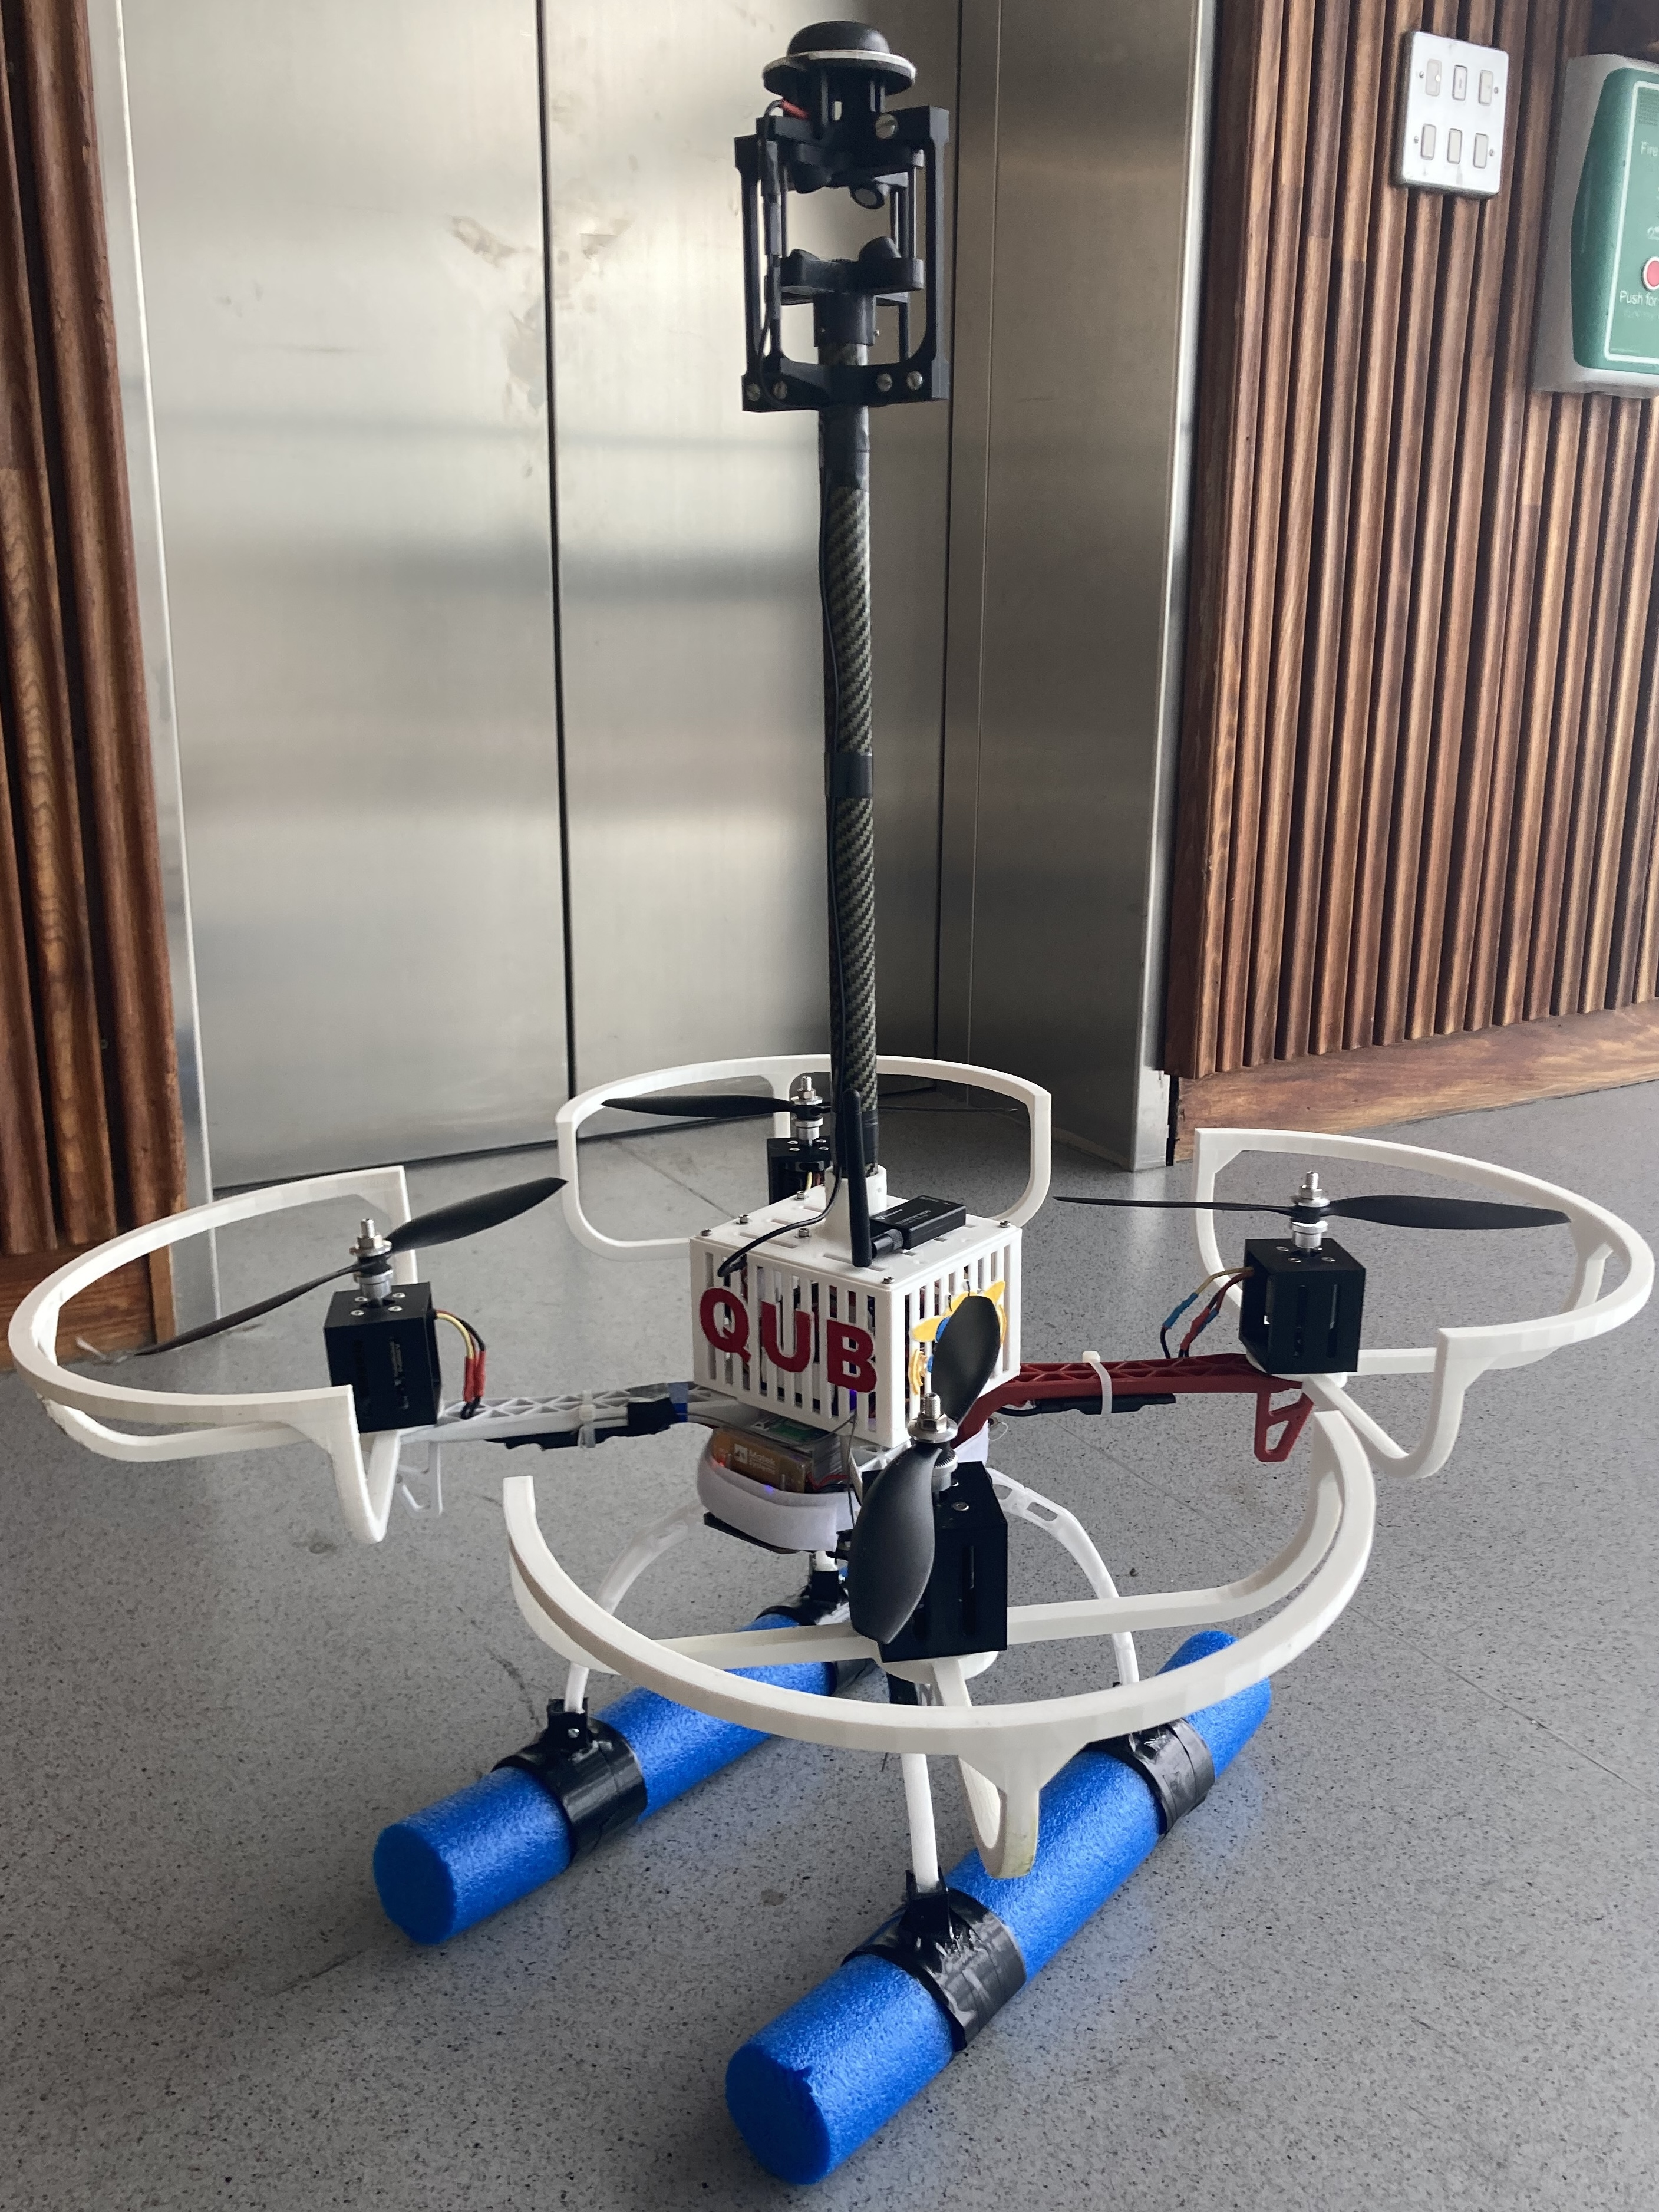
\includegraphics[width=0.35\textwidth]{Pictures/Quad.jpg} 
  \caption{Bzzz quadcopter}
  \label{fig:QuadDiagram}
\end{figure}

\noindent
The quadcopter is shaped like an 'X,' with each arm extending diagonally from the
center body, where the core components are housed. Here's a detailed overview of
its structure:
\subsection*{Frame}
\begin{figure}[H]
  \centering
  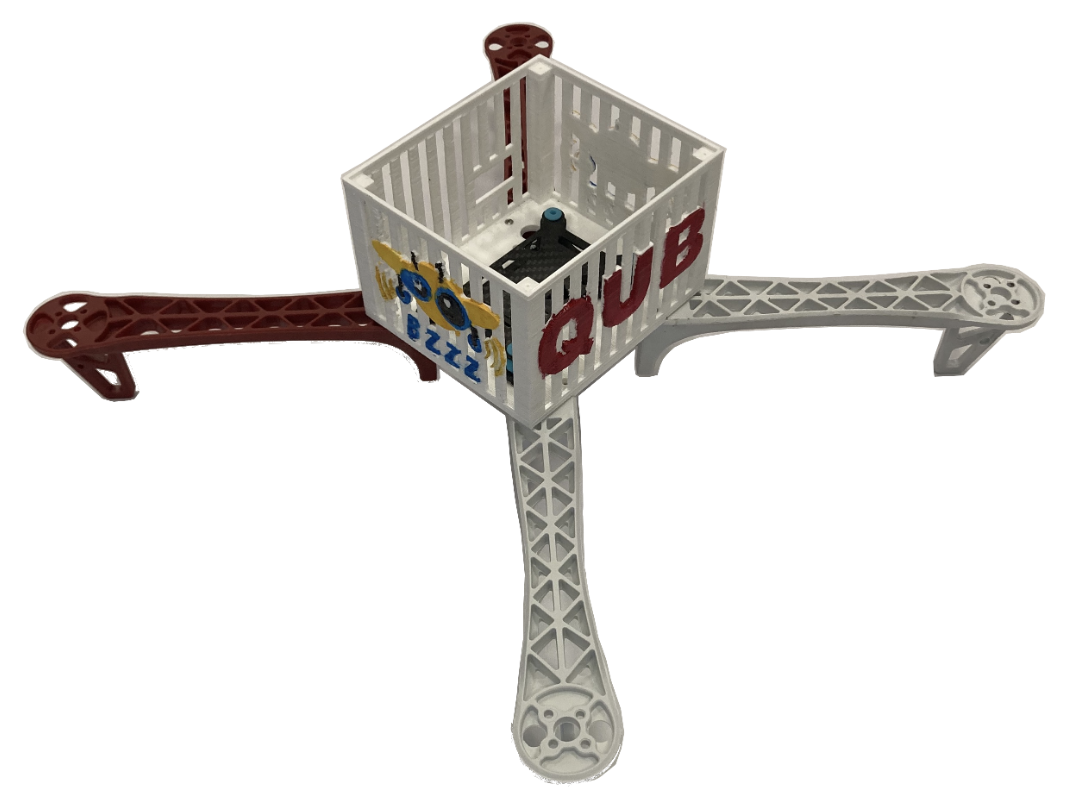
\includegraphics[width=0.35\textwidth]{Pictures/frame_housing.png} 
  \caption{Central hub attached to the arms}
  \label{fig:Central_hub_arms}
\end{figure}
\begin{itemize}
  \item \textbf{The Central Hub}, the quadcopter's central hub, houses vital
  parts required for its  functionality, making it crucial to its operation. The
  battery compartment is positioned inside this core in a way that maximises the
  quadcopter's centre of gravity and promotes steady and balanced flight
  dynamics. Mounting plates are essential for the quadcopter's operational
  capabilities and versatility as they offer safe attachment points
  for structural components like landing gear. Moreover, the landing gear
  attachments' direct integration into the hub allows for seamless and secure
  operations while strengthening the structure to withstand the stresses of
  takeoff and landing. The arrangement of parts inside the central hub improves
  the quadcopter's performance and maneuverability in addition to preserving its
  structural integrity.
  \item \textbf{The Arms}, four arms extend out of the central hub in an X
  configuration, this is where the motor housings are fastened, these housings
  are designed to accommodate the quadcopter's motors, protecting them from
  damage while ensuring they remain firmly attached, even under the stress of
  high-speed rotation and the various forces experienced during flight
  maneuvers. As well as the propeller guards, These guards serve as a protective
  barrier around the spinning propellers, safeguarding against accidental
  contact with objects or people. The guards help to prevent damage to the
  propellers and reduce the risk of injury from the spinning blades.
\end{itemize}

\subsection*{Landing gear}
\begin{figure}[H]
  \centering
  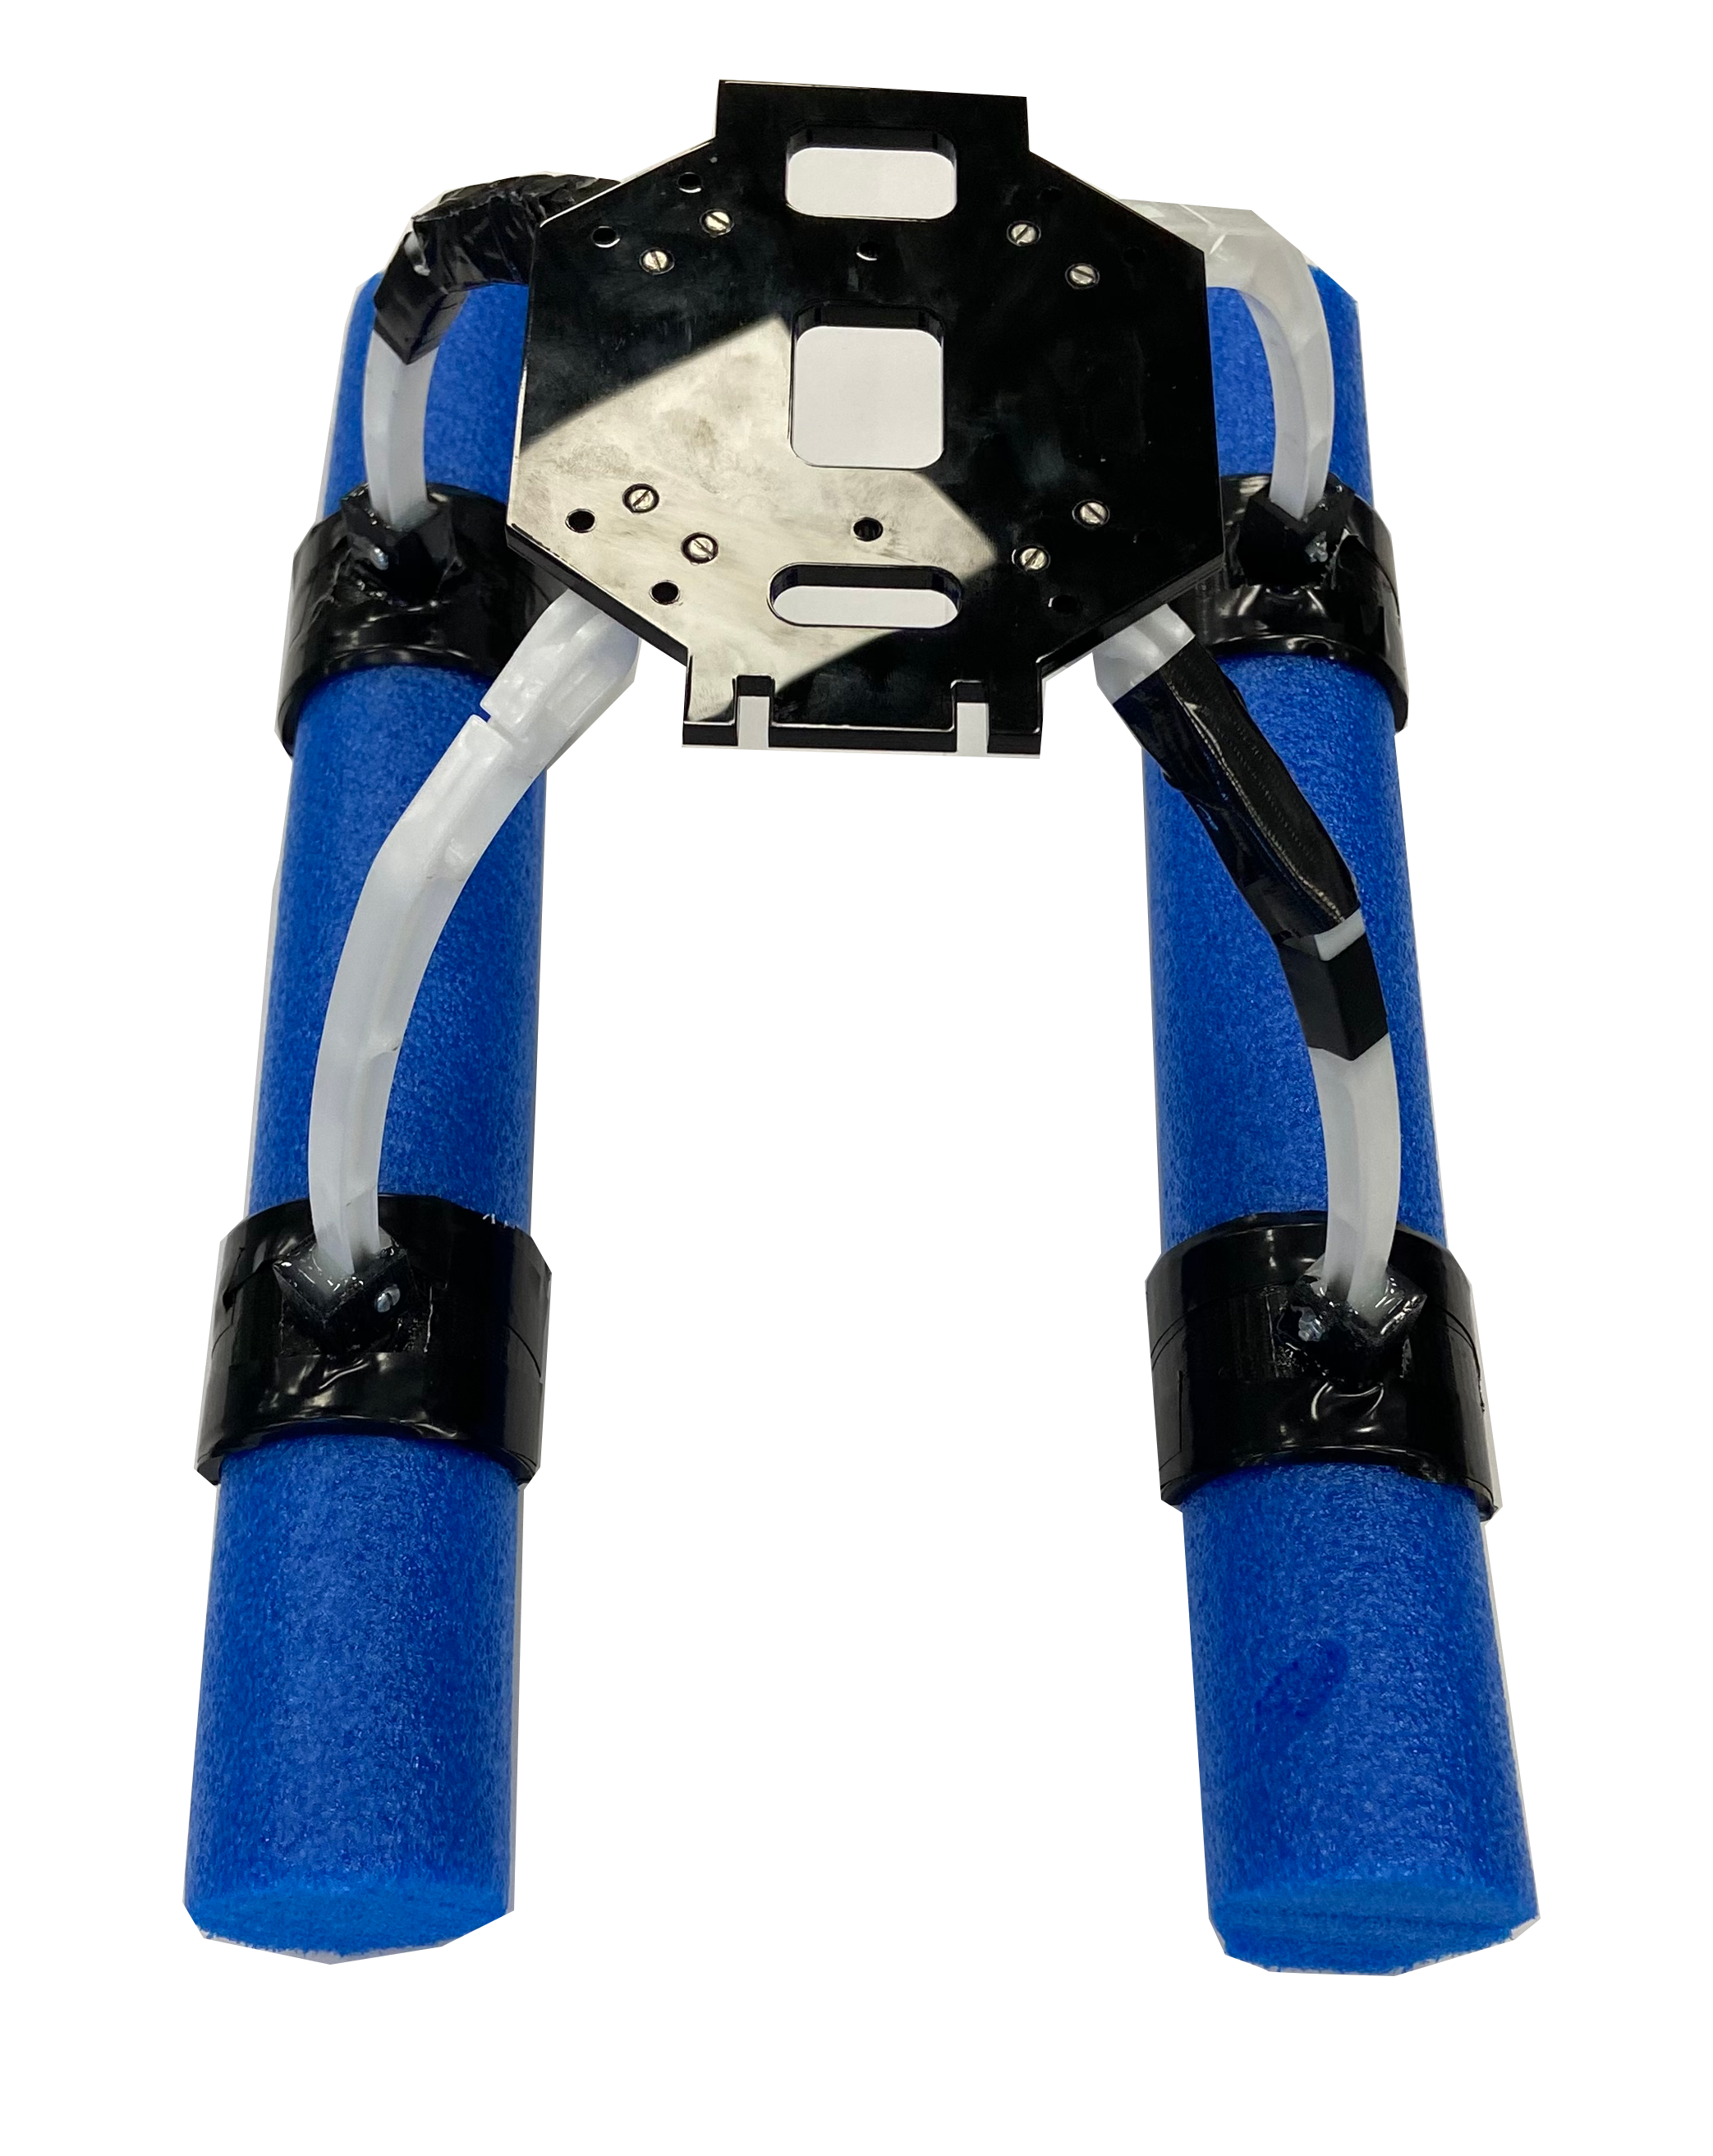
\includegraphics[width=0.35\textwidth]{Pictures/legs_baseplate.png} 
  \caption{Quadcopter legs feet and dampers}
  \label{fig:feet_dampers}
\end{figure}
\begin{itemize}
  \item \textbf{Quadcopters legs}, the four quadcopter legs are all the same
  length and run parallel to the arms from the central hub towards the ground.
  These stands are responsible for keeping the quadcopter horizontal for a
  smooth take off and landing. The stands also provide necessary clearance
  between the quadcopter's body (and potentially any attached components or
  sensors) and the ground. This clearance is important to prevent damage to the
  underside of the quadcopter and any sensitive equipment during landing or when
  taking off from uneven terrain.
  \item \textbf{Feet and Dampers}, the black feet which are fastened to the
  bottom of the stands ensure that the foam dampers are security fastened onto
  the bottom of the quad, taking a horse shoe like shape which matches the shape
  of the dampers. The dampers absorb the impact when the quadcopter lands. This
  helps protect the integrity of the frame and sensitive components from the
  shock and vibration that occur during landing, especially on hard or uneven
  surfaces. They are also used to reduce vibrations transmitted from the ground
  to the quadcopter's frame during landing and takeoff. By dampening these
  vibrations, the foam contributes to more stable take off and landings and
  helps protect onboard components.
\end{itemize}

\subsection*{Electronic housing}
\begin{figure}[H]
  \centering
  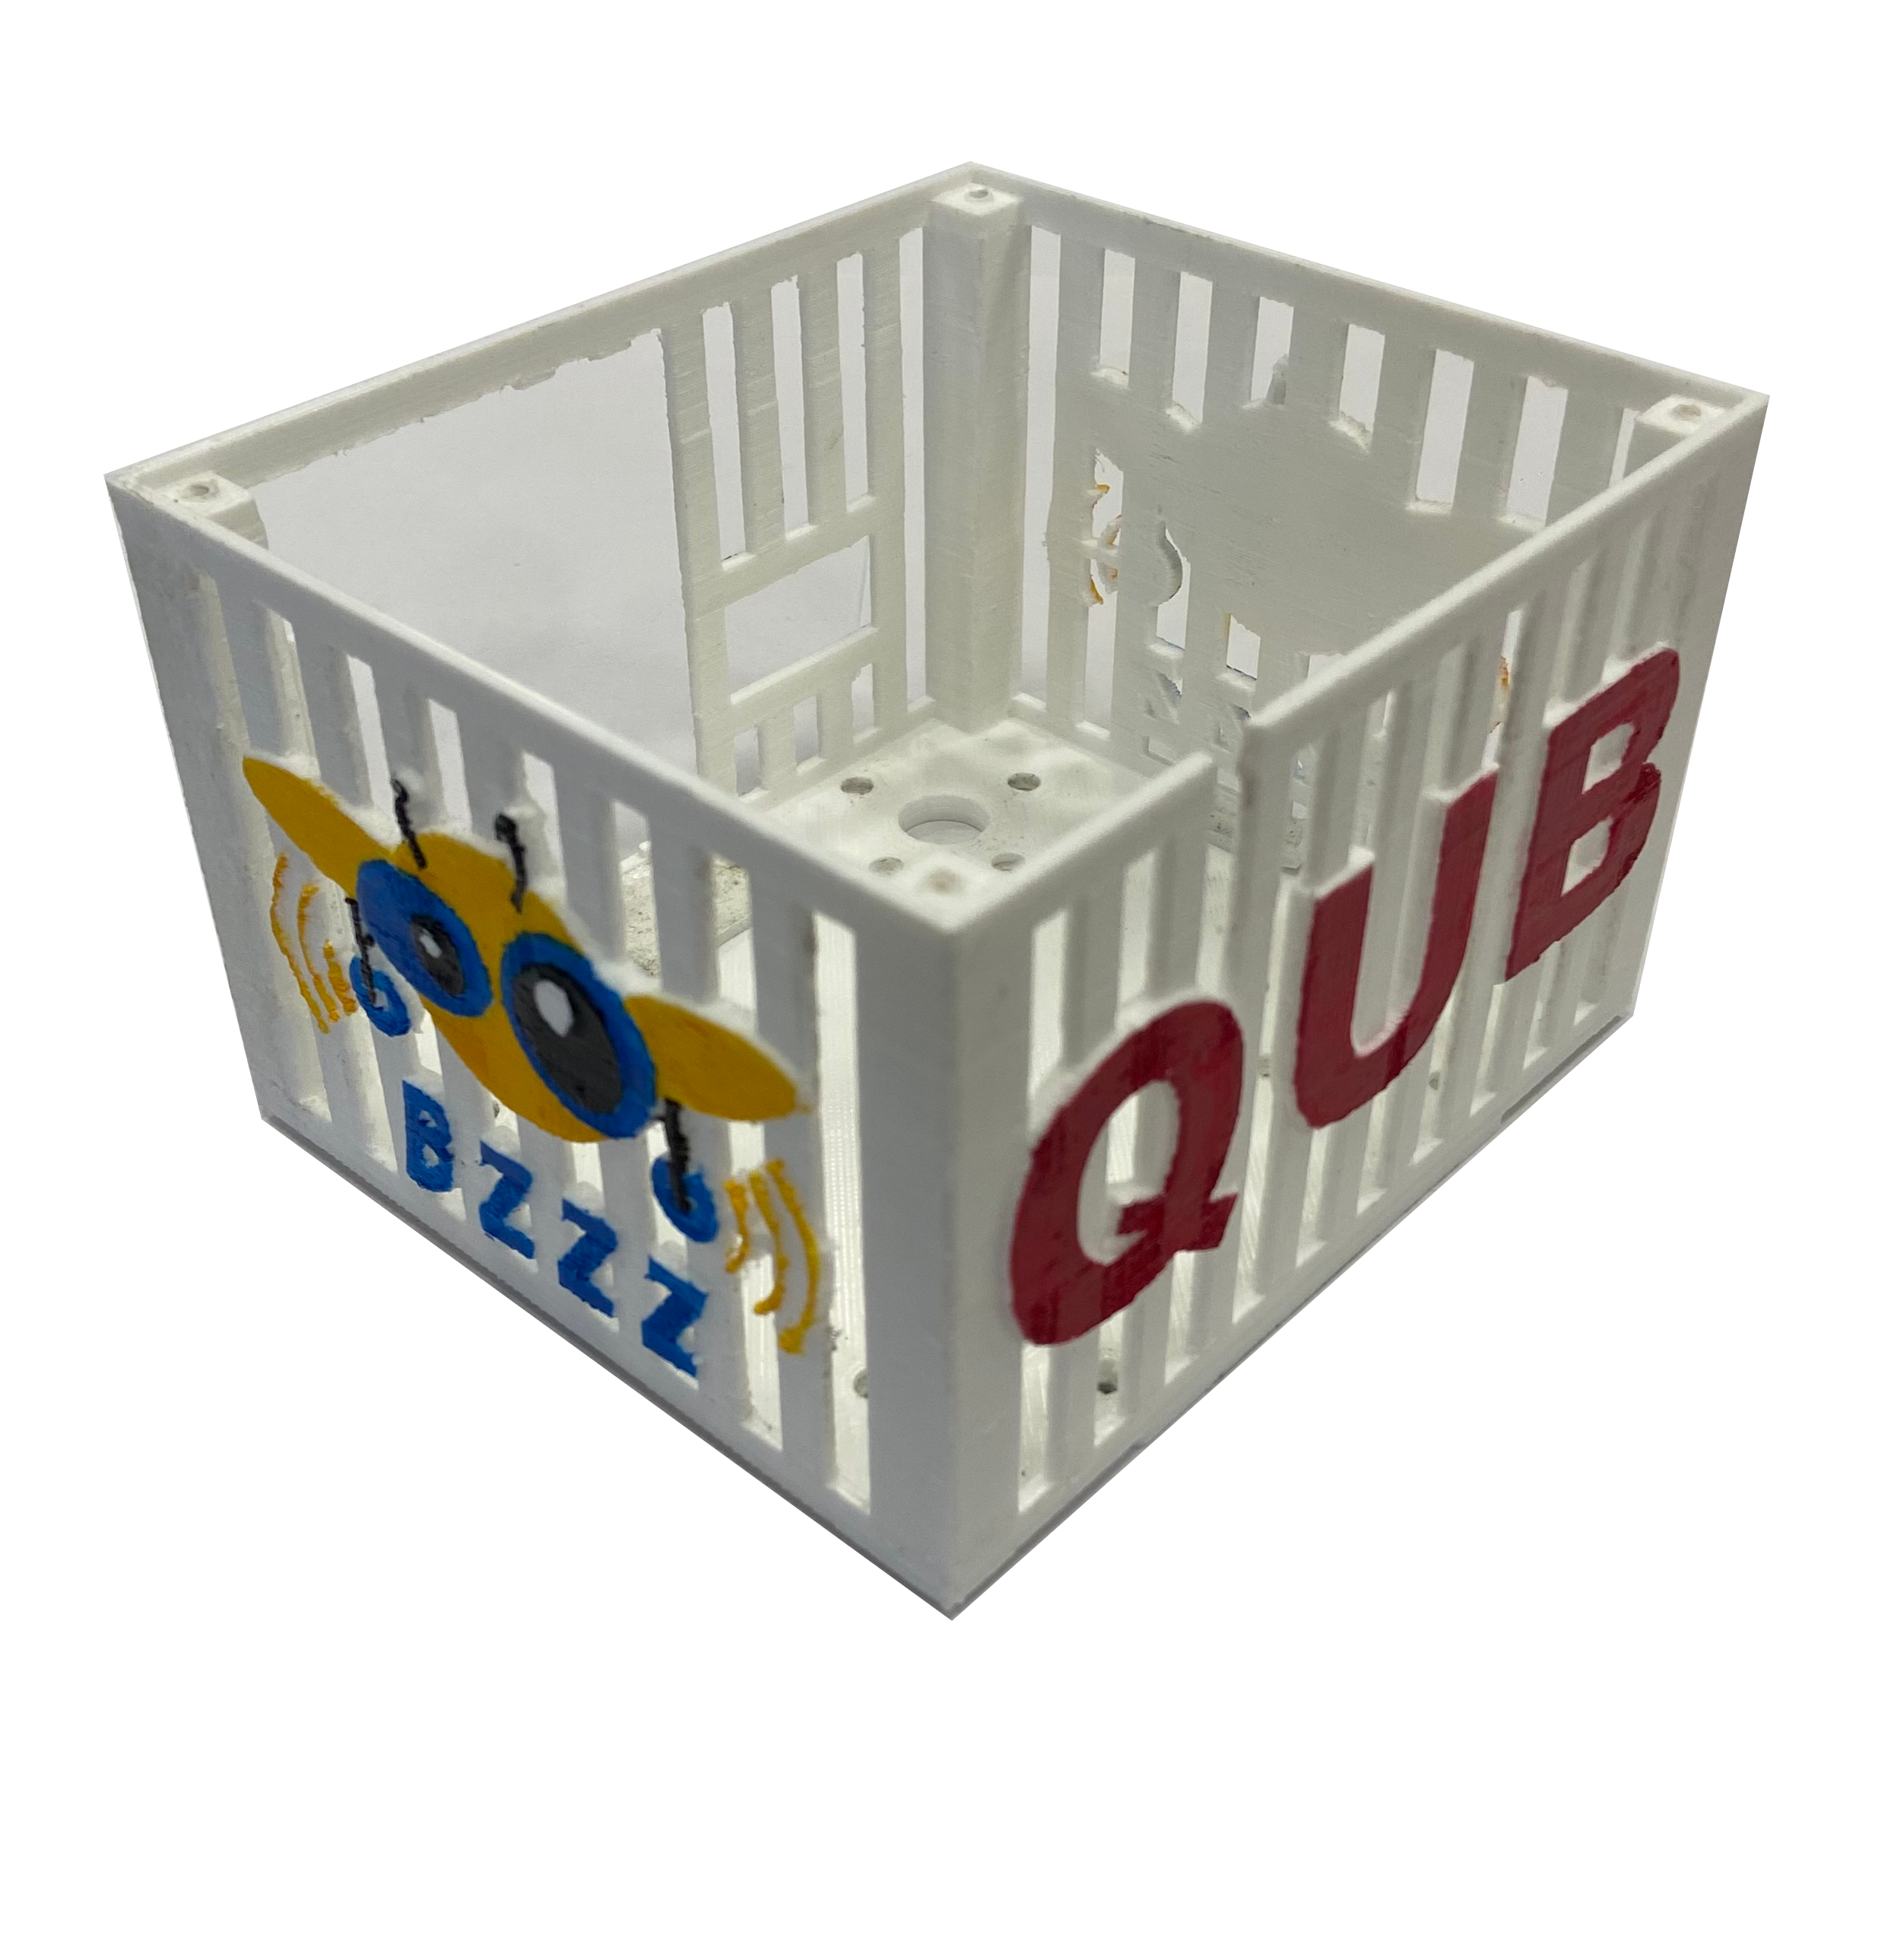
\includegraphics[width=0.35\textwidth]{Pictures/electronic_housing.png} 
  \caption{Electronic Housing}
  \label{fig:electronic_housing}
\end{figure}
The white caged electronic housing box is where the computational unit, an
Inertial Measurement Unit (IMU), Raspberry Pi, Radio receiver, GNSS rover module
and voltage regulator are all placed at the center of the body, situated above
the central hub. For more information on the electronic components used please
see section....
 
\section{Thrust Overview}
This section briefly runs over how the quadcopter produces thrust. A quadcopter
uses four separate brushless (BLDC) motors, each paired with a specific
electronic speed controllers (ESCs) that adjusts how fast the motor spins. These
controllers work by receiving a digital signal, known as Pulse-Width Modulation
(PWM) which have a pulse, the 'width' of these pulses (i.e., how long they stay
'on' versus 'off' in a given cycle) is adjusted to control the speed of the
motor. This is known as the duty cycle. A longer 'on' time (wider pulse) means
more power is delivered to the motor, making it spin faster. Digital
microcontrollers are typically used to create these PWM signals.

Propellers generate thrust through aerodynamic principles, primarily by
leveraging the pressure differential created by the airfoil-shaped blades as
they slice through the air. According to Bernoulli's principle, the acceleration
of air over the blade surfaces leads to a lower pressure on the top side
compared to the bottom, due to the faster flow of air this pressure difference
produces lift. This is a similar concept to an aircraft wing. Furthermore,
Newton's third law of motion: every action has an equal and opposite reaction,
should be considered as the propeller blades push air downwards, resulting in an
upward reactionary force. The efficiency of this process is influenced by the
propeller's angle of attack and the rotational speed, which determine the volume
of air displaced. However, factors such as viscous drag and turbulence can
reduce the thrust efficiency, necessitating aerodynamic optimizations to
minimize energy losses and maximise the generated thrust, see
Fig.\ref{fig:thrustconfig}.

On the quadcopter depicted in Fig.\ref{fig:QuadDiagram} and
Fig.\ref{fig:motorconfig} two motors spin in a clockwise direction and two in
the anticlockwise direction, motors which rotate in the same direction are
placed on opposite sides of the diagonal arms. The reason for this is to provide
stability and accurate control. By counteracting the angular momentum produced
by each motor, this arrangement keeps the quadcopter oriented and stops it from
spinning out of control. The quadcopter's stability is enhanced by the
deliberate positioning of motors rotating at the same speed on opposing diagonal
arms, which balances torque. Additionally, by adjusting the motors' rotational
speeds, this configuration makes it easier to perform yaw motions, which are
necessary for steering and adjusting orientation on the x-axis. This design
decision improves manoeuvrability and simplifies the entire structure, removing
the need for more intricate programming to resist rotating forces. As a result,
the control system becomes simpler and more effective through the use of the
ESC's.

\begin{figure}[htbp]
  \centering
  % First minipage for the first diagram
  \begin{minipage}{.5\textwidth}
    \centering
    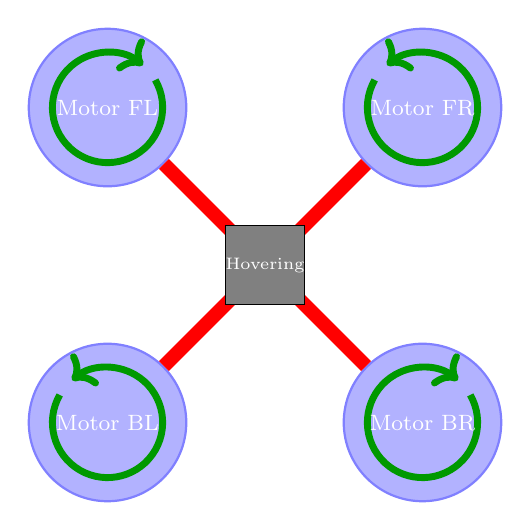
\begin{tikzpicture}[ motor/.style={circle, draw=blue!50, fill=blue!30,
      thick, minimum size=2cm}, hoverarc/.style={line width=2.5pt,
      green!60!black, ->}, body/.style={draw, fill=black!50, minimum width=1cm,
      minimum height=1cm}, ]
    
    % Motors
    \node[motor] (fl) at (0,0) {}; \node[motor] (fr) at (4,0) {}; \node[motor]
    (bl) at (0,-4) {}; \node[motor] (br) at (4,-4) {};
    
    % Hover speed arcs Clockwise motors
    \draw[hoverarc] (fl) ++(30:0.7) arc (30:-310:0.7); \draw[hoverarc] (br)
    ++(30:0.7) arc (30:-310:0.7);
    
    % Counterclockwise motors
    \draw[hoverarc] (fr) ++(150:0.7) arc (150:490:0.7); \draw[hoverarc] (bl)
    ++(150:0.7) arc (150:490:0.7);
    
    % Labels inside motors
    \node[text=white, font=\fontsize{8pt}{10pt}\selectfont] at (fl) {Motor FL};
    \node[text=white, font=\fontsize{8pt}{10pt}\selectfont] at (fr) {Motor FR};
    \node[text=white, font=\fontsize{8pt}{10pt}\selectfont] at (bl) {Motor BL};
    \node[text=white, font=\fontsize{8pt}{10pt}\selectfont] at (br) {Motor BR};
    
    % Diagonal lines
    \draw[line width=5pt, red] (fl) -- (br); \draw[line width=5pt, red] (fr) --
    (bl);
    
    % Black body in the center
    \node[body] (quad) at ($(fl)!.5!(br)$) {};

    % hovering label
    \node[text=white, font=\fontsize{6pt}{10pt}\selectfont] at (quad)
    {Hovering};
    
    \end{tikzpicture}
    \caption{Motor configuration top view.}
    \label{fig:motorconfig}
  \end{minipage}%
  % Second minipage for the second diagram
  \begin{minipage}{.5\textwidth}
    \centering
    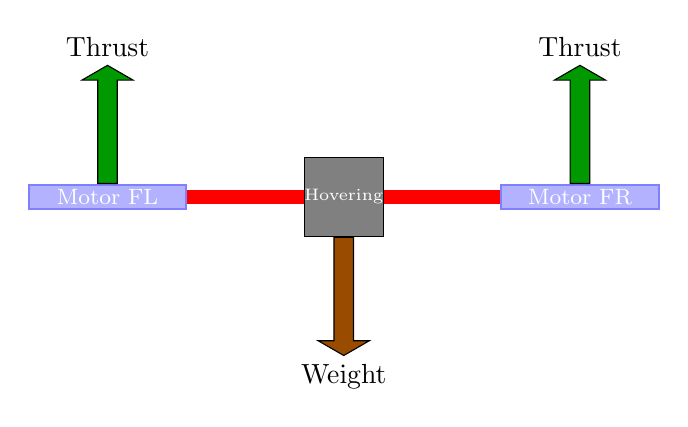
\begin{tikzpicture}[ propeller/.style={draw, draw=blue!50, fill=blue!30,
      thick, minimum width=2cm, minimum height=0.3cm}, body/.style={draw,
      fill=black!50, minimum width=1cm, minimum height=1cm},
      thrust/.style={single arrow, draw, fill=green!60!black, minimum
      height=1.5cm, minimum width=4mm, single arrow head extend=2mm, single
      arrow tip angle=120, shape border rotate=90}, weight/.style={single arrow,
      draw, fill=orange!60!black, minimum height=1.5cm, minimum width=4mm,
      single arrow head extend=2mm, single arrow tip angle=120, shape border
      rotate=270}, label/.style={text=white,
      font=\fontsize{8pt}{10pt}\selectfont} ]
    
    % Quadcopter body
    \node[body] (quad) {};
    
    % Propellers as seen from the side
    \node[propeller] (fl) at (-3,0) {}; \node[propeller] (fr) at (3,0) {};
    
    % Labels for propellers and body
    \node[label] at (fl) {Motor FL}; \node[label] at (fr) {Motor FR};
    
    % Arms, only two visible from the side view
    \draw[line width=5pt, red] (quad.west) -- (fl.east); \draw[line width=5pt,
    red] (quad.east) -- (fr.west);
    
    % Thrust arrows
    \node[thrust, anchor=tail] at (fl.north) {}; \node[thrust, anchor=tail] at
    (fr.north) {};

    % Weight arrow 
    \node[weight, anchor=tail] at (quad.south) {};
    
    % Thrust labels
    \node[anchor=south, yshift=1.5cm] at (fl.north) {Thrust};
    \node[anchor=south, yshift=1.5cm] at (fr.north) {Thrust};

    % Weight label
    \node[anchor=north, yshift=-1.5cm] at (quad.south) {Weight};

    % Hovering label
    \node[text=white, font=\fontsize{6pt}{10pt}\selectfont] at (quad)
    {Hovering};
    
    \end{tikzpicture}
    \caption{Side view of a quadcopter with motor thrust.}
    \label{fig:thrustconfig}
  \end{minipage}
\end{figure}
   
As we can see from the above diagrams in Fig.\ref{fig:motorconfig} and
Fig.\ref{fig:thrustconfig}, the motors are spinning at a rate at which the
thrust produced is greater than the weight of the quadcopter, allowing it to
hover. The direction of the thrust arrows in the diagrams indicates the rotation
of each propeller allowing a force exerted by each motor to counteract gravity
and maintain the quadcopter's hovering state. The balanced forces from opposite
motors, as depicted in the top view (Fig.\ref{fig:motorconfig}), ensure
stability and control, while the side view (Fig. \ref{fig:thrustconfig})
illustrates how the collective thrust from all motors must exceed the downward
force of the quadcopter's weight to achieve lift. This equilibrium between
thrust and weight is essential for the quadcopter to remain airborne and perform
various manoeuvres.

Please note that the diagrams produced are not to scale and are just for the
readers understanding on how the quadcopers thrust dynamics are produced.

\section{Quadcopter position
manipulation}\label{Quadcopter_position_manipulation} In this section we will go
through the quadcopters dynamics and how we can manipulate them in order to
manoeuvre the quad to achieve a specified position and or direction of flight

\begin{figure}[htbp]
  \centering
  \begin{tikzpicture}
    % Place the image in the document
    \node[anchor=south west, inner sep=0] (image) at (0,0)
    {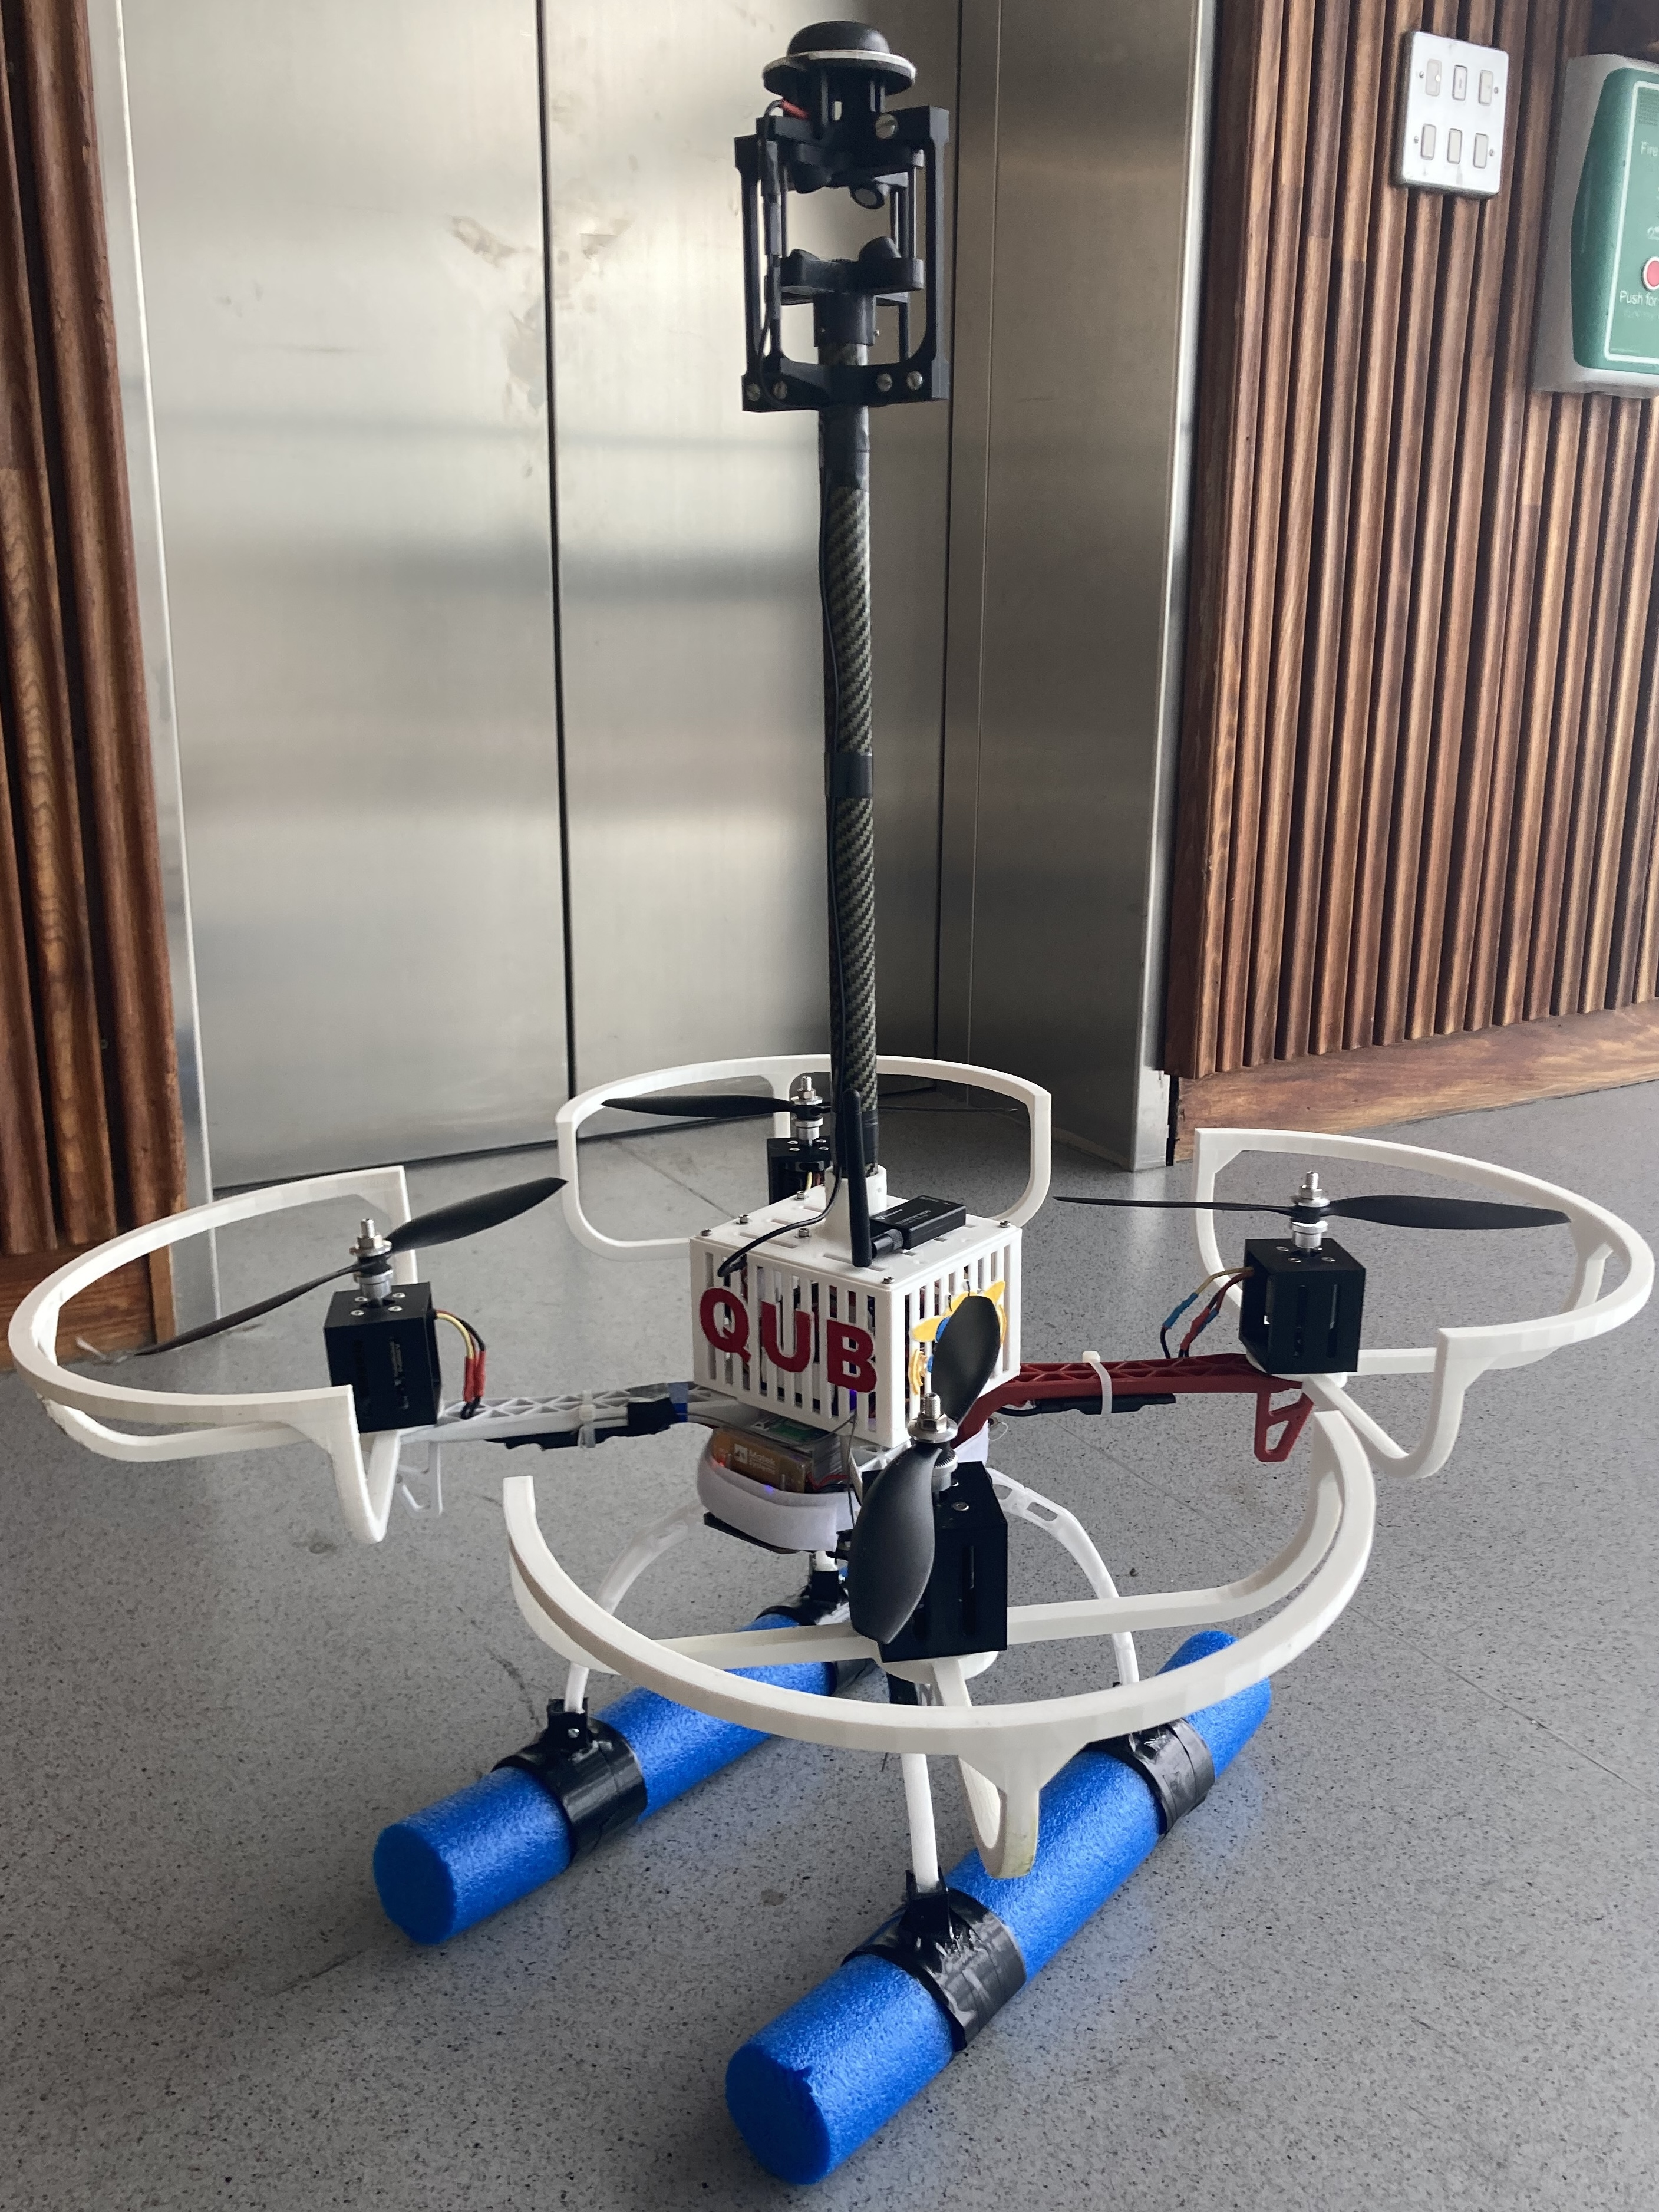
\includegraphics[width=0.45\textwidth]{Pictures/Quad.jpg}};
    % Set the origin of the diagram in the middle of the quadcopter
    \coordinate (O) at ($(image.south west)!0.5!(image.north east) + (0,-1cm)$);
  
    % Draw the axes x-axis
    \draw[->,line width=5pt,red] (O) -- ++(2,-0.5,0) node[anchor=west,
    font=\fontsize{15pt}{10pt}\selectfont]{$x$};
    % z-axis (previously y-axis)
    \draw[->,line width=5pt,blue] (O) -- ++(0,3,0) node[anchor=south, xshift=-0.2cm, font=\fontsize{15pt}{10pt}\selectfont]{$z$};
    % y-axis (previously z-axis)
    \draw[->,line width=5pt,green] (O) -- ++(0,1,5) node[anchor=east,
    font=\fontsize{15pt}{10pt}\selectfont]{$y$};
    % Add a label for 'Front'
    \node[text=white, font=\large] at ($(O) + (1.5,1.5,0)$) {Front};

    % Add a label for 'Back'
    \node[text=white, font=\large] at ($(O) + (-3,-1.5,0)$) {Back};

    % Add rotational arrows around each axis Around x-axis
    \draw[->,line width=2pt,red!60] ($(O) + (1,0.2,0)$) arc (90:360:0.2 and
    0.5);
    % Around y-axis
    \draw[->,line width=2pt,green!60] ($(O) + (-0.5,0.3,0.5)$) arc (90:360:0.2
    and 0.5);
    % Around z-axis
    \draw[->,line width=2pt,blue!60] ($(O) + (0.5,2,0)$) arc (40:310:0.5 and
    0.2);
  \end{tikzpicture}
  \caption{Quadcopter with pitch, roll and yaw axes.}
  \label{fig:quadwithaxis}
\end{figure}

\begin{enumerate}
  \item \textbf{Pitchx}, measured around a body fixed x-axis.
  \item \textbf{Roll}, measured around a body fixed y-axis.
  \item \textbf{Yaw} or heading, measured along a body fixed z-axis.
\end{enumerate}

\subsection{Electronic Speed Controllers (ESCs)}
Electronic Speed Controllers (ESCs) precisely control the speed of each rotor,
enabling pilots to execute complex pitch roll and yaw manoeuvres and retain
stability, even in challenging conditions. This is accomplished by computing the
difference in velocity that controls the rate of rotation between pairs of
rotors spinning clockwise and anticlockwise on every axis.

\subsection{Pitch}
Pitch control in a quadcopter is achieved through the manipulation of the
rotational speeds of its rotors (FL, FR, BL, BR Fig.\ref{fig:motorconfig}),
which in turn alters the thrust produced by each motor. To initiate a pitch
movement, which is a forward or backward tilt leading to forward or backward
movement, the quadcopter adjusts the speed of its front and rear rotors relative
to each other. 

To initiate a forward pitch, the rear rotors (BL and BR) are amplified to
produce additional lift at the back of the quadcopter. At the same time,
decelerating the front rotors reduces their lifting capacity in turn leading to
an uneven force distribution along x-axis which causes movement towards the
front direction as the thrust produced by the back motors is greater than that
of the front, this leads to a positive torque. Conversely, when executing a
backward pitch manoeuvre on a quadcopter, the front rotors (FL and FR) rotate at
an accelerated pace while the rear ones slow down, as the thrust produced by the
front motors is greater than that of the back, this leads to a negative torque
on the x-axis. This disparity in speed results in the unmanned aerial vehicle
leaning backwards.

The resulting torque produced on the x-axis is shown below:
\begin{equation}
  \tau_{x, total} = \frac{d}{\sqrt{2}} (T_{\text{FL}} + T_{\text{FR}} - T_{\text{BL}} - T_{\text{BR}})
  \label{torque_x}
\end{equation}

\noindent
Where, \(T_{FL}\),  \(T_{FR}\), \(T_{BL}\) and \(T_{BR}\) are forces of thrust by the motors, d is the distance of the center of mass from any one motor (length of the drones arm).

The torque calculation is affected by the leverage effect of the motor thrusts, namely the perpendicular distance between the centre and the line of action of each motor's thrust. Because the perpendicular distance in a square arrangement is smaller than the diagonal by a factor of 
\(\sqrt{2}\), the torque formula divides by \(\sqrt{2}\).
\begin{figure}[H]
  \centering
  % First minipage for the first figure
  \begin{minipage}{.5\textwidth}
    \centering
    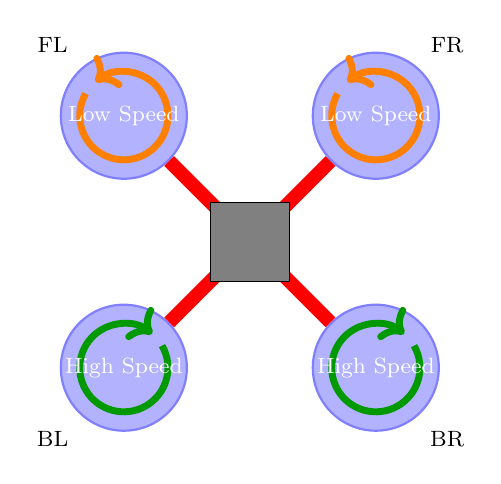
\begin{tikzpicture}[ scale=0.8, motor/.style={circle, draw=blue!50,
      fill=blue!30, thick, minimum size=1.6cm}, hoverarcgreen/.style={line
      width=2.5pt, green!60!black, ->}, hoverarcorange/.style={line width=2.5pt,
      orange!100, ->}, body/.style={draw, fill=black!50, minimum width=1cm,
      minimum height=1cm},
      motorlabel/.style={font=\fontsize{8pt}{12pt}\selectfont, text=black} ]
    
    % Motors
    \node[motor] (fl) at (0,0) {}; \node[motor] (fr) at (4,0) {}; \node[motor]
    (bl) at (0,-4) {}; \node[motor] (br) at (4,-4) {};
    
    % Hover speed arcs Clockwise motors
    \draw[hoverarcgreen] (bl) ++(30:0.7) arc (30:-310:0.7); \draw[hoverarcgreen]
    (br) ++(30:0.7) arc (30:-310:0.7);
    
    % Counterclockwise motors
    \draw[hoverarcorange] (fr) ++(150:0.7) arc (150:490:0.7);
    \draw[hoverarcorange] (fl) ++(150:0.7) arc (150:490:0.7);
    
    % Labels inside motors
    \node[text=white, font=\fontsize{8pt}{10pt}\selectfont] at (fl) {Low Speed};
    \node[text=white, font=\fontsize{8pt}{10pt}\selectfont] at (fr) {Low Speed};
    \node[text=white, font=\fontsize{8pt}{10pt}\selectfont] at (bl) {High
    Speed}; \node[text=white, font=\fontsize{8pt}{10pt}\selectfont] at (br)
    {High Speed};

    % Motor labels outside circles
    \node[motorlabel] at ($(fl)+(135:1.6)$) {FL}; \node[motorlabel] at
    ($(fr)+(45:1.6)$) {FR}; \node[motorlabel] at ($(bl)+(-135:1.6)$) {BL};
    \node[motorlabel] at ($(br)+(-45:1.6)$) {BR};
    
    % Diagonal lines
    \draw[line width=5pt, red] (fl) -- (br); \draw[line width=5pt, red] (fr) --
    (bl);
    
    % Black body in the center
    \node[body] (quad) at ($(fl)!.5!(br)$) {};
    
    \end{tikzpicture}
    \caption{Illustration of forward\\ pitch on quadcopter}
    \label{fig:forwardpitch}
  \end{minipage}%
  % Second minipage for the second figure
  \begin{minipage}{.5\textwidth}
    \centering
    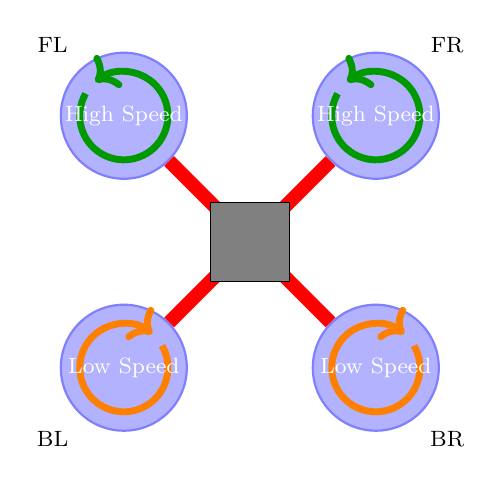
\begin{tikzpicture}[ scale=0.8, motor/.style={circle, draw=blue!50,
      fill=blue!30, thick, minimum size=1.6cm}, hoverarcgreen/.style={line
      width=2.5pt, green!60!black, ->}, hoverarcorange/.style={line width=2.5pt,
      orange!100, ->}, body/.style={draw, fill=black!50, minimum width=1cm,
      minimum height=1cm},
      motorlabel/.style={font=\fontsize{8pt}{12pt}\selectfont, text=black} ]
    % Motors
    \node[motor] (fl) at (0,0) {}; \node[motor] (fr) at (4,0) {}; \node[motor]
    (bl) at (0,-4) {}; \node[motor] (br) at (4,-4) {};
    
    % Hover speed arcs Clockwise motors
    \draw[hoverarcorange] (bl) ++(30:0.7) arc (30:-310:0.7);
    \draw[hoverarcorange] (br) ++(30:0.7) arc (30:-310:0.7);
    
    % Counterclockwise motors
    \draw[hoverarcgreen] (fr) ++(150:0.7) arc (150:490:0.7);
    \draw[hoverarcgreen] (fl) ++(150:0.7) arc (150:490:0.7);
    
    % Labels inside motors
    \node[text=white, font=\fontsize{8pt}{10pt}\selectfont] at (fl) {High
    Speed}; \node[text=white, font=\fontsize{8pt}{10pt}\selectfont] at (fr)
    {High Speed}; \node[text=white, font=\fontsize{8pt}{10pt}\selectfont] at
    (bl) {Low Speed}; \node[text=white, font=\fontsize{8pt}{10pt}\selectfont] at
    (br) {Low Speed};

    % Motor labels outside circles
    \node[motorlabel] at ($(fl)+(135:1.6)$) {FL}; \node[motorlabel] at
    ($(fr)+(45:1.6)$) {FR}; \node[motorlabel] at ($(bl)+(-135:1.6)$) {BL};
    \node[motorlabel] at ($(br)+(-45:1.6)$) {BR};
    
    % Diagonal lines
    \draw[line width=5pt, red] (fl) -- (br); \draw[line width=5pt, red] (fr) --
    (bl);
    
    % Black body in the center
    \node[body] (quad) at ($(fl)!.5!(br)$) {};

    \end{tikzpicture}
    \caption{Illustration of backward\\ pitch on quadcopter}
    \label{fig:backwordpitch}
  \end{minipage}
\end{figure}
Figure\ref{fig:forwardpitch} illustrates a pitch to the front of the quadcopter,
motors BL and BR are spinning faster than FL and FR. This leads to more thrust
being produced by the back two motors than the front two. This causes the
quadcopter to rotate in a clockwise motion along the x-axis.

On the other hand Figure\ref{fig:backwordpitch} illustrates a pitch to the back
of the quadcopter, motors FL and FR are spinning faster than BL and BR. This
leads to more thrust being produced by the front two motors than the back two.
This causes the quadcopter to rotate in a anti-clockwise motion along the
x-axis.

\subsection{Roll}
To manoeuvre the quadcopters roll, adjusting the speeds of its rotors is key.
This involves creating an imbalance, in thrust between either side of the
aircraft prompting it to tilt along its  y-axis depicted in
Fig.\ref{fig:quadwithaxis}. When initiating a roll to the right side the
quadcopter increases the speed of its left side rotors (FL and BL) while
decreasing that of its right side rotors (FR and BR). This disparity in thrust
causes a torque that tilts and rolls it to the right. Conversely, for a roll the
opposite occurs the quadcopter increases the speed of its right side rotors (FR
and BR) while decreasing that of its right side rotors (FL and BL). Through the
use of roll the quadcopter adjusts its orientation and gains movement in that
direction. 

The resulting torque produced on the y-axis is shown below:
\begin{equation}
  \tau_{y, total} = \frac{d}{\sqrt{2}} (T_{\text{FL}} + T_{\text{FR}} - T_{\text{BL}} - T_{\text{BR}}),
  \label{torque_y}
\end{equation}
where, \(T_{FL}\),  \(T_{FR}\), \(T_{BL}\) and \(T_{BR}\) are forces of thrust
by the motors, d is the distance of the center of mass from any one motor
(length of the drones arm).

\begin{figure}[H]
  \centering
  % First minipage for the first figure
  \begin{minipage}{.5\textwidth}
    \centering
    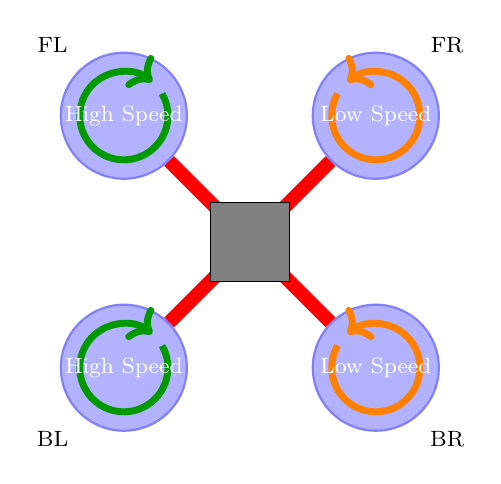
\begin{tikzpicture}[ scale=0.8, motor/.style={circle, draw=blue!50,
      fill=blue!30, thick, minimum size=1.6cm}, hoverarcgreen/.style={line
      width=2.5pt, green!60!black, ->}, hoverarcorange/.style={line width=2.5pt,
      orange!100, ->}, body/.style={draw, fill=black!50, minimum width=1cm,
      minimum height=1cm},
      motorlabel/.style={font=\fontsize{8pt}{12pt}\selectfont, text=black} ]
    
    % Motors
    \node[motor] (fl) at (0,0) {}; \node[motor] (fr) at (4,0) {}; \node[motor]
    (bl) at (0,-4) {}; \node[motor] (br) at (4,-4) {};
    
    % Hover speed arcs Clockwise motors
    \draw[hoverarcgreen] (bl) ++(30:0.7) arc (30:-310:0.7); \draw[hoverarcgreen]
    (fl) ++(30:0.7) arc (30:-310:0.7);
    
    % Counterclockwise motors
    \draw[hoverarcorange] (fr) ++(150:0.7) arc (150:490:0.7);
    \draw[hoverarcorange] (br) ++(150:0.7) arc (150:490:0.7);
    
    % Labels inside motors
    \node[text=white, font=\fontsize{8pt}{10pt}\selectfont] at (fl) {High
    Speed}; \node[text=white, font=\fontsize{8pt}{10pt}\selectfont] at (fr) {Low
    Speed}; \node[text=white, font=\fontsize{8pt}{10pt}\selectfont] at (bl)
    {High Speed}; \node[text=white, font=\fontsize{8pt}{10pt}\selectfont] at
    (br) {Low Speed};

    % Motor labels outside circles
    \node[motorlabel] at ($(fl)+(135:1.6)$) {FL}; \node[motorlabel] at
    ($(fr)+(45:1.6)$) {FR}; \node[motorlabel] at ($(bl)+(-135:1.6)$) {BL};
    \node[motorlabel] at ($(br)+(-45:1.6)$) {BR};
    
    % Diagonal lines
    \draw[line width=5pt, red] (fl) -- (br); \draw[line width=5pt, red] (fr) --
    (bl);
    
    % Black body in the center
    \node[body] (quad) at ($(fl)!.5!(br)$) {};
    
    \end{tikzpicture}
    \caption{Illustration of right roll on quadcopter}
    \label{fig:rightroll}
  \end{minipage}%
  % Second minipage for the second figure
  \begin{minipage}{.5\textwidth}
    \centering
    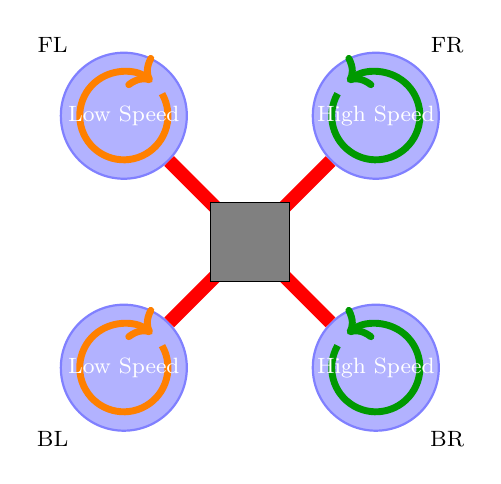
\begin{tikzpicture}[ scale=0.8, motor/.style={circle, draw=blue!50,
      fill=blue!30, thick, minimum size=1.6cm}, hoverarcgreen/.style={line
      width=2.5pt, green!60!black, ->}, hoverarcorange/.style={line width=2.5pt,
      orange!100, ->}, body/.style={draw, fill=black!50, minimum width=1cm,
      minimum height=1cm},
      motorlabel/.style={font=\fontsize{8pt}{12pt}\selectfont, text=black} ]
    % Motors
    \node[motor] (fl) at (0,0) {}; \node[motor] (fr) at (4,0) {}; \node[motor]
    (bl) at (0,-4) {}; \node[motor] (br) at (4,-4) {};
    
    % Hover speed arcs Clockwise motors
    \draw[hoverarcorange] (fl) ++(30:0.7) arc (30:-310:0.7);
    \draw[hoverarcorange] (bl) ++(30:0.7) arc (30:-310:0.7);
    
    % Counterclockwise motors
    \draw[hoverarcgreen] (br) ++(150:0.7) arc (150:490:0.7);
    \draw[hoverarcgreen] (fr) ++(150:0.7) arc (150:490:0.7);
    
    % Labels inside motors
    \node[text=white, font=\fontsize{8pt}{10pt}\selectfont] at (fr) {High
    Speed}; \node[text=white, font=\fontsize{8pt}{10pt}\selectfont] at (fl) {Low
    Speed}; \node[text=white, font=\fontsize{8pt}{10pt}\selectfont] at (br)
    {High Speed}; \node[text=white, font=\fontsize{8pt}{10pt}\selectfont] at
    (bl) {Low Speed};

    % Motor labels outside circles
    \node[motorlabel] at ($(fl)+(135:1.6)$) {FL}; \node[motorlabel] at
    ($(fr)+(45:1.6)$) {FR}; \node[motorlabel] at ($(bl)+(-135:1.6)$) {BL};
    \node[motorlabel] at ($(br)+(-45:1.6)$) {BR};
    
    % Diagonal lines
    \draw[line width=5pt, red] (fl) -- (br); \draw[line width=5pt, red] (fr) --
    (bl);
    
    % Black body in the center
    \node[body] (quad) at ($(fl)!.5!(br)$) {};

    \end{tikzpicture}
    \caption{Illustration of left roll on quadcopter}
    \label{fig:leftroll}
  \end{minipage}
\end{figure}

Figure\ref{fig:rightroll} illustrates a roll to the right of the quadcopter,
motors FL and BL are spinning faster than FR and BR. This leads to more thrust
being produced by the two left motors than the two right. This discrepancy in
thrust causes the quadcopter to rotate in a clockwise motion along the y-axis.

On the other hand Figure\ref{fig:leftroll} illustrates a roll to the left of the
quadcopter, motors FR and BR are spinning faster than FL and BL. This leads to
more thrust being produced by the two right motors than the two left motors.
This discrepancy in thrust causes the quadcopter to rotate in a anti-clockwise
motion along the y-axis.

\subsection{Yaw}
By adjusting rotor speeds, one may precisely control a quadcopter's yaw, or
rotation about the vertical z-axis (see Fig.\ref{fig:quadwithaxis}). To do this,
opposing diagonal rotors must rotate at different speeds in order to produce
torque, which causes rotation around the vertical axis.

The quadcopter rotates clockwise when viewed from above, it achieves this by
increasing the speed of the counter-clockwise (FL and BR) and reducing the speed
of the clockwise (FR and BL) (Fig.\ref{fig:motorconfig}) spinning rotors. This
generates positive (upward) torque that turns it to the right. this torque can
be represented by \(\tau_{cw}\).

Similar adjustments are performed to the rotor speeds for an anticlockwise or
leftward movement: FR and BL spin more quickly as FL and BR slow down,
generating an overall negative (downward) torque \(\tau_{acw}\) causing the
quadcopter to turn to the left.

The resultant torque of the overall model from can be given by:
\begin{equation}
  \tau_{z, total} = \tau_{acw} - \tau_{cw}
  \label{total_torque}
\end{equation}

The direction of motion can be determined form torque by using, the Right-Hand
Rule: Point your right hand's fingers in the direction of the position vector
(from the axis of rotation to the point where force is applied). Curl them
toward the direction of the force. Your thumb points in the direction of the
torque vector. If your thumb points out of the page (towards you), the torque is
anti-clockwise (acw), leading to anti-clockwise motion. If your thumb points
into the page (away from you), the torque is clockwise (cw), leading to
clockwise motion.

Expanding on the idea of using torque to determine motion direction, it's vital
to acknowledge that a system comprising several motors (FL, FR, BL, BR)  can
have its total torque analysed by breaking the system down into individual
torques generated by each motor. The sum of the individual reaction torques
produced by each motor is represented in the Equation below. 
\begin{equation}
  \begin{bmatrix}
    \tau_{acw}\\
    \tau_{cw}
  \end{bmatrix} = 
  \begin{bmatrix}
    \tau_{FL} + \tau_{BR}\\
    \tau_{FR} + \tau_{BL}
  \end{bmatrix}
\end{equation}

\begin{figure}[H]
  \centering
  % First minipage for the first figure
  \begin{minipage}{.5\textwidth}
    \centering
    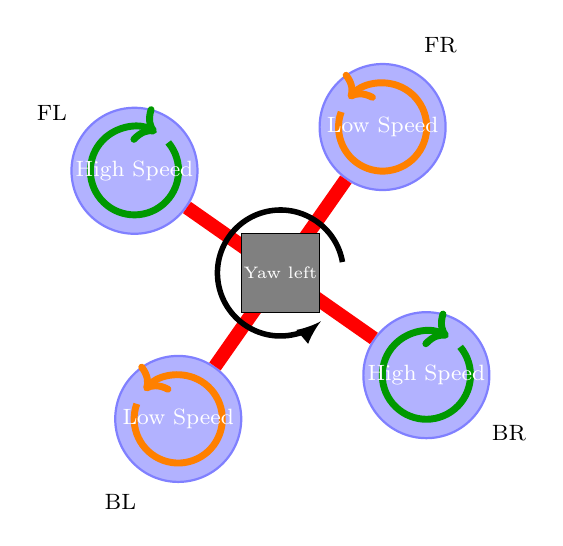
\begin{tikzpicture}[ scale=0.8, rotate=10,
      % Rotate the entire drawing by 10 degrees
      motor/.style={circle, draw=blue!50, fill=blue!30, thick, minimum
      size=1.6cm}, hoverarcgreen/.style={line width=2.5pt, green!60!black, ->},
      hoverarcorange/.style={line width=2.5pt, orange!100, ->},
      body/.style={draw, fill=black!50, minimum width=1cm, minimum height=1cm},
      centerarrow/.style={->, >=latex, black, line width=2pt},
      motorlabel/.style={font=\fontsize{8pt}{12pt}\selectfont, text=black} ]
    
    % Motors
    \node[motor] (fl) at (0,0) {}; \node[motor] (fr) at (4,0) {}; \node[motor]
    (bl) at (0,-4) {}; \node[motor] (br) at (4,-4) {};
    
    % Hover speed arcs Clockwise motors
    \draw[hoverarcgreen] (fl) ++(30:0.7) arc (30:-310:0.7); \draw[hoverarcgreen]
    (br) ++(30:0.7) arc (30:-310:0.7);
    
    % Counterclockwise motors
    \draw[hoverarcorange] (fr) ++(150:0.7) arc (150:490:0.7);
    \draw[hoverarcorange] (bl) ++(150:0.7) arc (150:490:0.7);
    
    % Labels inside motors
    \node[text=white, font=\fontsize{8pt}{10pt}\selectfont] at (fl) {High
    Speed}; \node[text=white, font=\fontsize{8pt}{10pt}\selectfont] at (fr) {Low
    Speed}; \node[text=white, font=\fontsize{8pt}{10pt}\selectfont] at (bl) {Low
    Speed}; \node[text=white, font=\fontsize{8pt}{10pt}\selectfont] at (br)
    {High Speed};

    % Motor labels outside circles
    \node[motorlabel] at ($(fl)+(135:1.6)$) {FL}; \node[motorlabel] at
    ($(fr)+(45:1.6)$) {FR}; \node[motorlabel] at ($(bl)+(-135:1.6)$) {BL};
    \node[motorlabel] at ($(br)+(-45:1.6)$) {BR};
    
    % Diagonal lines
    \draw[line width=5pt, red] (fl) -- (br); \draw[line width=5pt, red] (fr) --
    (bl);
    
    % Black body in the center
    \node[body] (quad) at ($(fl)!.5!(br)$) {};
    
    % Central red arrow
    \draw[centerarrow] ($(quad)+(1,0)$) arc (0:300:1);
    
    \node[text=white, font=\fontsize{6pt}{10pt}\selectfont] at ($(quad)+(0,0)$)
    {Yaw left};
    
    \end{tikzpicture}
    \caption{Illustration of acw yaw on quadcopter}
    \label{fig:first-acwyaw}
  \end{minipage}%
  % Second minipage for the second figure
  \begin{minipage}{.5\textwidth}
    \centering
    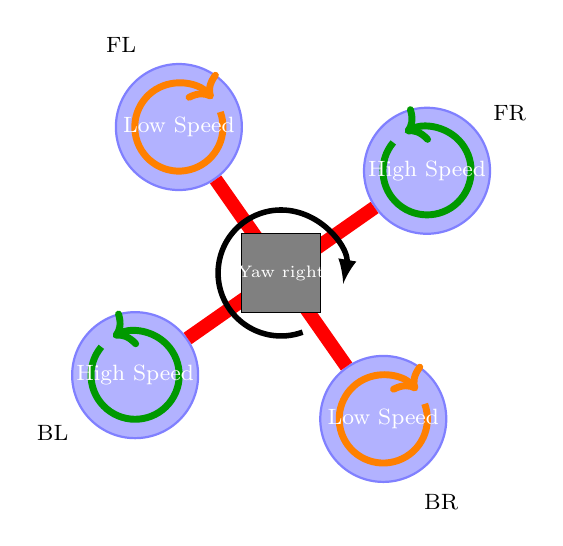
\begin{tikzpicture}[ scale=0.8, rotate=-10,
      % Rotate the entire drawing by 10 degrees
      motor/.style={circle, draw=blue!50, fill=blue!30, thick, minimum
      size=1.6cm}, hoverarcgreen/.style={line width=2.5pt, green!60!black, ->},
      hoverarcorange/.style={line width=2.5pt, orange!100, ->},
      body/.style={draw, fill=black!50, minimum width=1cm, minimum height=1cm},
      centerarrow/.style={<-, >=latex, black, line width=2pt},
      motorlabel/.style={font=\fontsize{8pt}{12pt}\selectfont, text=black} ]
    % Motors
    \node[motor] (fl) at (0,0) {}; \node[motor] (fr) at (4,0) {}; \node[motor]
    (bl) at (0,-4) {}; \node[motor] (br) at (4,-4) {};
    
    % Hover speed arcs Clockwise motors
    \draw[hoverarcorange] (fl) ++(30:0.7) arc (30:-310:0.7);
    \draw[hoverarcorange] (br) ++(30:0.7) arc (30:-310:0.7);
    
    % Counterclockwise motors
    \draw[hoverarcgreen] (fr) ++(150:0.7) arc (150:490:0.7);
    \draw[hoverarcgreen] (bl) ++(150:0.7) arc (150:490:0.7);
    
    % Labels inside motors
    \node[text=white, font=\fontsize{8pt}{10pt}\selectfont] at (fl) {Low Speed};
    \node[text=white, font=\fontsize{8pt}{10pt}\selectfont] at (fr) {High
    Speed}; \node[text=white, font=\fontsize{8pt}{10pt}\selectfont] at (bl)
    {High Speed}; \node[text=white, font=\fontsize{8pt}{10pt}\selectfont] at
    (br) {Low Speed};

    % Motor labels outside circles
    \node[motorlabel] at ($(fl)+(135:1.6)$) {FL}; \node[motorlabel] at
    ($(fr)+(45:1.6)$) {FR}; \node[motorlabel] at ($(bl)+(-135:1.6)$) {BL};
    \node[motorlabel] at ($(br)+(-45:1.6)$) {BR};
    
    % Diagonal lines
    \draw[line width=5pt, red] (fl) -- (br); \draw[line width=5pt, red] (fr) --
    (bl);
    
    % Black body in the center
    \node[body] (quad) at ($(fl)!.5!(br)$) {};
    
    % Central red arrow
    \draw[centerarrow] ($(quad)+(1,0)$) arc (0:300:1);
    
    \node[text=white, font=\fontsize{6pt}{10pt}\selectfont] at ($(quad)+(0,0)$)
    {Yaw right};

    \end{tikzpicture}
    \caption{Illustration of cw yaw on quadcopter}
    \label{fig:second-cwyaw}
  \end{minipage}
\end{figure}

In both of the above diagrams Fig.\ref{fig:first-acwyaw} and
Fig.\ref{fig:second-cwyaw} show the cw and acw yaw mechanics.
Fig.\ref{fig:first-acwyaw} shows a yew to the left, this is due to the fact that
motors, FL and BR are running faster than the motors FR and BL this produces a
positive total torque as a result of equation \ref{total_torque}, this in turn,
will cause the quadcopter to yaw in an anti-clockwise direction (to the left).

Conversely, Fig.\ref{fig:second-cwyaw}  shows a yew to the right, this is due to
the fact that motors, FR and BL are running faster than the motors FL and BR
this produces a negative total torque as a result of equation
\ref{total_torque}, this in turn,  will cause the quadcopter to yaw in a
clockwise direction (to the Right).

Finally when all motors spin at the same rate the resultant total torque
(\(\tau_{total}\)) is zero, resulting in the quadcopter staying stationary.


Ultimately, Pitch, Roll and Yaw processes work together seamlessly to enhance
the quadcopters manoeuvrability during flights for more accurate adjustments in
orientation as required throughout each journey.

\subsection{IMU (Inertial Measurement Unit)}
An Inertial Measurement Unit (IMU) is a crucial part of electronics that
combines a magnetometer, accelerometer, and gyroscope. The accelerometer
measures changes in velocity along linear axes in metres per second squared,
while the gyroscope tracks rotational motion in degrees per second and finally,
the magnetometer measures magnetic field strength in micro-Teslas. Through the
use of an advanced digital filter such as the Madgwick filter, the IMU is able to precisely determine the
orientation of the quadcopter. Using the IMU in this way guarantees accurate
orientation data, which is essential for quadcopter applications. More
details into the IMU which is being used can be seen below (see Section:\ref{IMU})

\subsection{Flight controller}
Controlling the pitch roll and yaw motions of the quadcopter is a crucial
responsibility of the flight controller. It processes the IMU data to understand
the vehicle's orientation and motion, then makes decisions to adjust the motors
and stabilize the flight. For more information on the flight controller
see Section:\ref{flight_controller}

\section{Control and Estimation}\label{control_and_estimation} During this
project the development of a kalman filter for position estimation on the z-axis
was paramount for sensor fusion. On the quadcopter there is a downward- facing
time-of-flight (ToF) sensor, which is an infrared distance sensor that measures
the distance from the ground with a standard error of ±6 cm. The quadcopter
carries a barometer which by measuring the barometric pressure can give an
estimate of the altitude (where the altitude is zero at sea level); the standard
error of this sensor is ±25cm. The quadcopter is also equipped with a GNSS
(global navigation satellite system) sensor, which uses the ZED-FP9 module. The
GNSS module is couples with a base GNSS station, which allows it to produce
accurate position estimates. The GNSS can estimate the altitude of the vehicle
(with respect to the sea level) with a standard error of ±5 cm. for more
information on the sensors used see Section:\ref{hardware}.
\subsection{Quaternions}
Building on the foundational principles of pitch, yaw, and roll seen in
Section\ref{Quadcopter_position_manipulation}, the system dynamics of a
quadcopter extend into the realm of intricate motion control and stability
mechanisms. A typical quadcopter can manoeuvre on any axis fixed to its frame,
it can ascend or descend vertically, and move laterally in the (x, y) plane of a
known global reference frame. The quadcopter's ability to move in a variety of
ways enables it to precisely navigate  aerial waypoints, adapting seamlessly to
both the immediate environment and the pilot's commands. 

A quaternion is a mathematical entity that extends complex numbers,
characterized by a four-dimensional vector space. It can be depicted through
various notations; the following expressions illustrate two commonly recognised
methods. The operation of quaternion multiplication is inherently
non-commutative, mirroring the nature of rotational operations. The components
of a quaternion labelled as \( q_1 \) to \( q_3 \) constitute its vector
component, whereas \( q_0 \) serves as its scalar component. As seen below,
\begin{align}
  q =& q_0 + {q_1}i + {q_2}j + {q_3}k \\
  q =& [q_0 + q_1 + q_2 + q_3]^T
\end{align}
The elements \(i , j\) and \(k\) satisfy the properties \( i^2 = j^2 = k^2 = ijk
= -1 \). A quaternion with a norm equal to 1 this can be used to represent a
rotation of the quadcopter. Specifically, one can express a unit quaternion with
the formula \( q = \cos \left(\frac{\theta}{2}\right) + \left(i\hat{n}_x +
j\hat{n}_y + k\hat{n}_z\right) \sin \left(\frac{\theta}{2}\right), \) depicting
a rotational transformation about the unit vector \(\hat{n} = (\hat{n}_x, \hat{n}_y, \hat{n}_z)\)
through an angle \( \theta \). By conversion, the quaternion \(e = 1 + 0i + 0j +
0k \) denotes the identity rotation, signifying no change in orientation,
aligned with the standard orientation of the quadcopter.

The multiplication of two quaternions, labelled as \( p \) and \( q \), is
executed through the Kronecker product, denoted by \( \otimes \). The resulting
quaternion is outlined in the equations that follow. When \( p \) is associated
with a specific rotation and \( q \) with another, the product \( p \otimes q \)
yields the resultant rotation combining both. It is pivotal to highlight that
the multiplication process for quaternions is inherently non-commutative,
mirroring the non-commutative characteristic of rotations themselves. The
bilinear operation \( p \otimes q \) is equal to the matrix \(Q(p)q\) as seen
below:
\begin{equation}
  p \otimes q = 
  \begin{bmatrix}
    p_0 & -p_1 & -p_2 & -p_3 \\
    p_1 & p_0 & -p_3 & p_2 \\
    p_2 & p_3 & p_0 & -p_1 \\
    p_3 & -p_2 & p_1 & p_0 \\
\end{bmatrix}
\begin{bmatrix}
    q_0 \\
    q_1 \\
    q_2 \\
    q_3 \\
\end{bmatrix}
\end{equation}
equivocally, 
\begin{equation}
  q \otimes p = 
  \begin{bmatrix}
    q_0 & -q_1 & -q_2 & -q_3 \\
    q_1 & q_0 & q_3 & -q_2 \\
    q_2 & -q_3 & q_0 & q_1 \\
    q_3 & q_2 & -q_1 & q_0 \\
\end{bmatrix}
\begin{bmatrix}
    p_0 \\
    p_1 \\
    p_2 \\
    p_3 \\
\end{bmatrix}
\end{equation}

Normalizing a quaternion ensures its magnitude (or norm) remains equal to one,
which is crucial for maintaining the quaternion's representation of rotation. A
normalized quaternion \( q \) can be obtained by dividing the quaternion by its
norm, where the norm \( \|q\| \) is defined as:

\begin{equation}
\|q\| = \sqrt{q_0^2 + q_1^2 + q_2^2 + q_3^2}.
\end{equation}

The conjugate of a quaternion \( q = q_0 + q_1i + q_2j + q_3k \) is given by:

\begin{equation}
q^* = q_0 - q_1i - q_2j - q_3k.
\end{equation}
similarly,
\begin{equation}
q^* = \begin{bmatrix} q_0 - q_1 - q_2 - q_3\end{bmatrix}^\intercal
\end{equation}

The inverse \( q^{-1} \) of a unit quaternion is equal to its conjugate over its
norm squared:

\begin{equation}
q^{-1} = \frac{q^*}{\|q\| ^2}
\end{equation}

This property simplifies the computation of the inverse for unit quaternions and
is particularly useful in rotational transformations.

Quaternions are extensively used in the stabilization and control of
quadcopters. For instance, the desired rotation \( q_d \) can be achieved by
applying a control torque \( \tau \) based on the error between the desired and
current quaternion \( q \):

\begin{equation}
  \tau = -K_p (q \otimes q_d^* - 1) - K_d \dot{q},
\end{equation}

\noindent
where \( K_p \) and \( K_d \) are the proportional and derivative gains, \(q \otimes q_d^*\) calculates the quaternion error by determining the rotation from the desired orientation to the current orientation. one in the equation represents the quaternion identity, which signifies no rotation, respectively.

For deeper insights into quaternion mathematics and its applications in
aerospace and robotics, consider exploring the following resources
\cite{Kuipers1999} \cite{quaternion_curves}
\cite{QuaternionBasedAttitudeControl}

\subsection{Attitude dynamics}
Attitude dynamics refers to the study and control of the orientation and
rotation of the quadcopter as it moves through the air. It encompasses
understanding how the quadcopter's attitude (its orientation with respect to an
inertial frame of reference, usually the Earth) changes in response to various
forces and moments applied to it. furthermore, how to control these changes to
achieve desired orientations and flight paths.

The attitude dynamics of the quadcopter are modelled by two quaternion dynamic
equations:
\begin{align}
    \dot{q} &= \frac{1}{2} \otimes q\begin{bmatrix} 0 \\ \omega \end{bmatrix}, \label{3d_oriantation_quaternion}\\
    \dot{\omega} &= I_{cm}^{-1} \cdot \tau - I_{cm}^{-1} \left[ \omega \times (I_{cm} \cdot \omega) \right] \label{angular_velocity}
\end{align}
Equation\eqref{3d_oriantation_quaternion} uses quaternions to handle the orientation of the quadcopter in 3D space. Quaternions are an
alternative to Euler angles and avoid the problem of gimbal lock, making them
favourable for applications like quadcopter control where orientation needs to
be tracked continuously and smoothly. \(\dot{q}\) represents the time derivative
of the quaternion, essentially describing how the orientation changes over time,
\(q\) represents the current orientation of the quaternion equation and
\(\omega\) is the angular velocity vector of the quadcopter taken from the IMU
around (\(x, y, z\)) respectively.

Equation\eqref{angular_velocity} describes how the angular velocity (\(\omega\))
of the quadcopter changes over time, denoted by \(\dot \omega\). \(I_{cm}\) is
the moment of inertia matrix, which describes how the mass of the quadcopter is
distributed relative to the center of mass (cm) around each of its axes and
\(I_{cm}^{-1}\) is the  inverse of the moment of inertia matrix, which is used
to calculate the angular acceleration from the applied torques (\(\tau\)).

Both equations(\eqref{3d_oriantation_quaternion}) and (\eqref{angular_velocity}) were
derived and changed from \cite{QuaternionBasedAttitudeControl}

\subsection{Altitude control}\label{Altitude_control} The altitude dynamics
of a quadcopter are defined within a global coordinate system, crucial for
maintaining a predetermined altitude from the Earth's surface. The model that
describes these dynamics is based on fundamental principles, delineated as
follows:

The rate of change of the quadcopter's altitude, represented as \( \dot{z}_t \),
is the result of the vertical acceleration \( a^z_{T_t} \) produced by the
quadcopter's motors at a given time minus the gravitational acceleration, \( g
\). This equation is continuous in time and is expressed as,
\begin{equation}
\dot{z}_t = a^z_{T,t} - g
\end{equation}\label{vertical acceleration}
\noindent
Here, \( a^z_{T_t} \) signifies the upward acceleration generated by the
propulsion at time \( t \), measured in meters per second squared. The constant
\( g \) denotes the acceleration due to Earth's gravity, also in meters per
second squared. The altitude \( z_t \) represents the quadcopter's center of
mass's vertical position at time \( t \), measured in meters.

Additionally, the quadcopter's vertical velocity \( v_{z_t} \) and vertical
acceleration \( a_{z_t} \) are defined by the rate of altitude change \(
\dot{z}_t \) and the rate of vertical acceleration change \( \dot{a}^z_{T_t} - g
\), respectively. The term \( \dot{a}^z_{T_t} \) is derived from the
quadcopter's upward thrust and serves as the system's input, while \( g \) is
considered a constant input in the opposite direction.

Let \( y_{t}^z = z_t \) be the output equation of the system. 

\subsubsection*{Modelling}
  The two main forces acting on the quadcopter are the weight, $mg$, and the
  force from the propellers, $F_{\rm prop}$, which has been found to depend
  linearly on the throttle reference signal $\tau\in[0,1]$. The throttle
  reference signal is a signal that is sent to the electronic speed controllers
  (ESCs) of the four motors; at $\tau=0$ the motors do not spin, whereas
  $\tau=1$ corresponds to the maximum rotation speed.
  
  In an experiment, the quadcopter was placed on digital scales and the lift (in
  $\unit{g}$) was measured for different values of $\tau$. The experimental
  results are shown in Figure:\ref{fig:liftpwm}, from which it seems that a
  reasonable model for the lifting force is
  \begin{equation}
    F_{\rm prop} = \alpha_0 \tau + \beta_0,
    \label{eq:Fprop}
  \end{equation}
  where $\alpha_0>0$ and $\beta_0<0$ are constants, which depend on the level of
  charge of the battery. Although the values of $\alpha_0$ and $\beta_0$ can be
  estimated from the data shown in Figure:\ref{fig:liftpwm}, their exact value
  is unknown while flying.
  
  \begin{figure}[h!]
    \centering
    \begin{tikzpicture}
      \begin{axis}[ width= 2.2in, height=1.2in, scale only axis, ylabel={Lift
          (g)}, xlabel={Throttle reference (\%)}, xmajorgrids, ymajorgrids,
          ylabel near ticks, xmin=10, xmax=40, ymin=0, ymax=2500, legend
          columns=1, legend style={fill=white, fill opacity=0.4, text opacity=1,
          font=\scriptsize}, legend style={at={(axis cs:10.5,2450)},anchor=north
          west}, legend cell align={left}, ]
  
        \addplot[mark=x, blue, only marks, line width=1.2pt]
        table [x=throttle_percentage, y=weight_decrease, col sep=comma]
          {Data/1045_full.csv}; \addlegendentry{Full battery ($R^2=99.99\%$)};
  
        \addplot[mark=none, blue!50, only marks, line width=1.2pt, mark=x]
        table [x=throttle_percentage, y=weight_decrease, col sep=comma]
          {Data/1045_low.csv}; \addlegendentry{Low battery ($R^2=90.1\%$)};
  
  
        \addplot[domain=0:50, blue, dashed]
        table [x=throttle_percentage, y = {create col/linear regression =
          {y=weight_decrease}}, col sep=comma] {Data/1045_full.csv}; \addplot[no
          marks, blue, dashed,
          domain=0:50]{\pgfplotstableregressiona*x+\pgfplotstableregressionb};
  
        \addplot[domain=0:50, blue!50, dashed]
        table [x=throttle_percentage, y = {create col/linear regression =
          {y=weight_decrease}}, col sep=comma] {Data/1045_low.csv}; \addplot[no
          marks, blue!50, dashed,
          domain=0:50]{\pgfplotstableregressiona*x+\pgfplotstableregressionb};
  
      \end{axis}
    \end{tikzpicture}
    \caption{Static lift (g) plotted against throttle reference (\%).}
    \label{fig:liftpwm}
  \end{figure}

  From the model of Equation \eqref{eq:Fprop}, the total acceleration is
  \begin{equation}
    a
    {}={}
    \frac{F_{\rm prop} - mg}{m}
    {}={}
    \frac{\alpha_0 \tau + \beta_0 - mg}{m}
    {}={}
    \frac{\alpha_0}{m} + \frac{\beta_0 - mg}{m}
    {}={}
    \alpha \tau + \beta,
  \end{equation}
  where,
  \begin{equation}\label{eq:alpha}
    \alpha = \alpha_0/m
  \end{equation}
  and
  \begin{equation}\label{eq:beta}
    \beta = (\beta_0 - mg) / m
  \end{equation}
  
  As a result, a dynamical model of the system is
  \begin{equation}
    \ddot{z} {}={} a \Leftrightarrow \ddot{z} {}={} \alpha \tau + \beta,
  \end{equation}
  where $z$ denotes the altitude of the quadcopter. Note again, that the exact
  values of the coefficients $\beta$ and $\alpha$ are not known while flying
  (but we will estimate them). We can write this model as
  \begin{subequations}
    \begin{align}
      \dot{z} {}={} & v,
      \\
      \dot{v} {}={} & \alpha \tau + \beta,
    \end{align}
  \end{subequations}
  where $v$ is the quadcopter's vertical velocity. By discretising, using
  Euler's discretisation, with sampling time $T_s$, we have
  \begin{subequations}\label{eq:basic-mdl}
    \begin{align}
      z_{t+1} {}={} & z_t + T_s v_t.
      \\
      v_{t+1} {}={} & v_t + T_s(\alpha \tau_t + \beta).
    \end{align}
  \end{subequations}
  The sampling time is $T_s = \unit[100]{ms}$. Note that this system is at
  equilibrium whenever $\alpha \tau_t + \beta = 0$, that is, equivalently,
  $\tau_t = -\beta / \alpha$. This defines the \textit{hovering throttle
  signal}, $\tau^{\rm eq} = -\beta / \alpha$.


    \subsubsection*{Estimator Design}\label{estimator_design}
    \subsubsection*{State Vector Definition}
    The state vector \( x_t \) is defined as,
    \begin{equation}
        x_t = 
        \begin{bmatrix}
            z_t &
            v_{t} & 
            \beta_t & 
            \alpha_t &
            d{_t}^{\rm bar}&
            d{_t}^{\rm Tof}&
        \end{bmatrix}
        \label{stateVectorXt}
    \end{equation}

    in order to compute the throttle signal \(\theta\) values for \(z, v, \alpha\) and \(\beta\) need to be estimated. These measurements often are subject to noise, therefore the system dynamics are seen below,
    \begin{align}
        z_{t+1} =& z_t + {T_s}{v_t} + w^{z}_{t}\\
        v_{t+1}^z =& v_t^z + T_s (\alpha_t \tau_t + \beta_t) + w_t^v\\
        \beta_{t+1} {}={} & \beta_t + w^\beta_t,\\
        \alpha_{t+1} {}={} & \alpha_t + w^\alpha_t.\\
    \end{align}

    We define $w_t^z$ and $w_t^v$ as the process noise elements. $w_t^z$ is
    distributed normally with zero mean and variance $\sigma_z^2$, expressed as
    $w_t^z \sim \mathcal{N}(0, \sigma_z^2)$, and similarly, $w_t^v$ follows a
    normal distribution with $w_t^v \sim \mathcal{N}(0, \sigma_v^2)$.
    Additionally, $w_t^\alpha$ and $w_t^\beta$ represent white noise processes
    with distributions $w_t^\alpha \sim \mathcal{N}(0, T_s \sigma_\alpha^2)$ and
    $w_t^\beta \sim \mathcal{N}(0, T_s \sigma_\beta^2)$ respectively. The
    system state to be estimated is denoted by $x_t = (z_t, v_t^z,
    \alpha_t, \beta_t)$, with the The state update equation \( x_{t+1} \) is defined as,
    \begin{equation}
        x_{t+1} = A_t x_t,
    \end{equation}

    \subsubsection*{State transition matrix \( A_t \)}
    The state transition matrix \( A \) describes how the state at time \( t \)
    evolves to the state at time \( t+1 \). For the given system. Given the
    state vector \( x_t = \begin{bmatrix} z_t&  v_t^z&  \alpha_t&  \beta_t&
    d_{bar}& d_{ToF} \end{bmatrix} \) \eqref{stateVectorXt} and output \(y_t =
    \begin{bmatrix} y^{gnss}_t & y^{ToF}_t& y^{bar}_t \end{bmatrix} \), the
    state transition matrix \( A_t \) from the system's dynamic model is defined
    as:
    \begin{equation}
    A_t = 
    \begin{bmatrix}
    1 & T_s & 0 & 0 & 0 & 0\\
    0 & 1 & T_s \tau_t & T_s & 0 & 0\\
    0 & 0 & 1 & 0 & 0 & 0 \\
    0 & 0 & 0 & 1 & 0 & 0 \\
    0 & 0 & 0 & 0 & 1 & 0 \\
    0 & 0 & 0 & 0 & 0 & 1 \\
    \end{bmatrix}
    \end{equation}
    where \( T_s \) is the sampling time, and \( \tau_t \) represents the
    throttle signal at time \( t \).
  
    \begin{equation}
      x_{t+1} = 
      \begin{bmatrix}
        1 & T_s & 0 & 0 & 0 & 0\\
        0 & 1 & T_s \tau_t & T_s & 0 & 0\\
        0 & 0 & 1 & 0 & 0 & 0 \\
        0 & 0 & 0 & 1 & 0 & 0 \\
        0 & 0 & 0 & 0 & 1 & 0 \\
        0 & 0 & 0 & 0 & 0 & 1 \\
      \end{bmatrix}
      x_t + w_t
    \end{equation}

    \subsubsection*{Process Noise Covariance Matrix \( Q \)}
    The process noise covariance matrix \( Q \) represents the covariance of the
    process noise, accounting for the uncertainty in the model dynamics:
    \begin{equation}
    Q = 
    \begin{bmatrix}
    \sigma_z^2 & 0 & 0 & 0 & 0 & 0 \\
    0 & \sigma_v^2 & 0 & 0 & 0 & 0 \\
    0 & 0 & T_s \sigma_\alpha^2 & 0 & 0 & 0 \\
    0 & 0 & 0 & T_s \sigma_\beta^2 & 0 & 0 \\
    0 & 0 & 0 & 0 & \sigma^2_{d_{ToF}} & 0 \\
    0 & 0 & 0 & 0 & 0 & \sigma^2_{d_{bar}} \\
    \end{bmatrix}
    \end{equation}
    Here, \( \sigma_z^2 \), \( \sigma_v^2 \), \( \sigma_\alpha^2 \), \(
    \sigma_\beta^2 \), \( \sigma^2_{d_{ToF}} \) and \( \sigma^2_{d_{bar}} \)
    represent the variances of the altitude, velocity, and the coefficients \(
    \alpha \) and \( \beta \), which relate the throttle signal to the lift.

    \subsubsection*{Outputs}
    The output \(y\) is shown by the following,

    \begin{equation}
    y = [y^{gnss}, y^{Tof}, y^{bar}]
    \end{equation}

    for the barometer sensor's output, denoted by \( y_{bar} \), is described
    by the equation,
    \begin{equation}
    y^{bar} = z + d^{bar} + w^{bar}
    \end{equation}
    where, 
    \begin{equation}
        d^{bar}_{t+1} = d^{bar}_t + w_{t}^{d^{bar}}
    \end{equation}
    The bias $(d^{bar})$ should stay consistent throughout readings, the second
    reading of the bias should be equal to the first allowing for some
    additional noise/offset.

    For the GPS (GNSS module) sensor's output, denoted by \( y^{gnss} \), is
    described by the equation,
    \begin{subequations}
        \begin{align}
            y^{gnss} 
            {}={}&
            z + w^{gnss} 
        \end{align}
    \end{subequations}

    The Time-of-Flight (ToF) sensor's output, denoted by \( y^{ToF} \), is
    described by the equation, which is equal to the altitude plus a bias term
    plus the measurement noise; overall,
    \begin{equation}
    y^{ToF} = z + d^{ToF} + w^{ToF}
    \end{equation}
    where we assume that \(d^{tof}\) is described by a simple model of the form
    t
    \begin{equation}
    d^{tof}_{t+1} = d^{tof}_t + w^{tof}_t
    \end{equation}

    Through all sensors \( y \) represents the output from the sensor. The
    variable \( z \) signifies the quadcopter's altitude, which is the
    measurement for all sensors. The term \( w \) encapsulates the measurement
    noise or errors associated with the sensors. This noise term, \( w \),
    encompasses various factors such as sensor inaccuracies, the impact of
    environmental conditions on sensor performance, and any systematic bias that
    might be inherent in the sensor's readings.

    \subsubsection*{Measurement Matrix \( C \)}
    The measurement matrix \( C \) links the state vector to the measurement
    vector:
    \begin{equation}
    C = 
    \begin{bmatrix}
    1 & 0 & 0 & 0 & 0 & 0 \\
    1 & 0 & 0 & 0 & 0 & 1 \\
    1 & 0 & 0 & 0 & 1 & 0 \\
    \end{bmatrix}
    \end{equation}
    This matrix considers the direct measurement of altitude by all sensors and
    accounts for biases in the ToF and barometer sensors. Were the first row represents the GNSS sensor, the second represents the ToF and the third represents the barometer

    The measurement model is defined as
    \begin{equation}
    y_t = C x_t + w_t
    \end{equation}
    \begin{equation}
        y_t  = 
        \begin{bmatrix}
            1 & 0 & 0 & 0 & 0 & 0 \\
            1 & 0 & 0 & 0 & 0 & 1 \\
            1 & 0 & 0 & 0 & 1 & 0 \\
        \end{bmatrix}
            x_t + w_t
    \end{equation}
    were, \(y_t\) is the current update.

    \subsubsection*{Measurement Noise Covariance Matrix \( R \)}
    The measurement noise covariance matrix \( R \) accounts for the uncertainty
    in sensor measurements:
    \begin{equation}
    R = 
    \begin{bmatrix}
    \sigma_{gnss}^2 & 0 & 0 \\
    0 & \sigma_{ToF}^2 & 0 \\
    0 & 0 & \sigma_{bar}^2
    \end{bmatrix}
    \end{equation}
    where \( \sigma_{bar}^2 \), \( \sigma_{gnss}^2 \), and \( \sigma_{ToF}^2 \)
    are the variances of the measurement noises for the barometer, GPS, and
    Time-of-Flight sensors, respectively.


\subsubsection*{Kalman filter equations}
The Kalman filter equations for the above system are:
\begin{align}
    \text{Measurement} &
    \left[
    \begin{array}{l}
      \hat{x}_{t{}\mid{}t}
      {}={}
      \hat{x}_{t{}\mid{}t-1}
      {}+{}
      \Sigma_{t{}\mid{}t-1}C^\intercal
      (C\Sigma_{t{}\mid{}t-1}C^\intercal + R)^{-1}(y_t - C\hat{x}_{t{}\mid{}t-1})
      \\
      \Sigma_{t{}\mid{}t}
      {}={}
      \Sigma_{t{}\mid{}t-1}
      {}-{}
      \Sigma_{t{}\mid{}t-1}C^\intercal
      (C\Sigma_{t{}\mid{}t-1}C^\intercal + R)^{-1}
      C\Sigma_{t{}\mid{}t-1}
    \end{array}
    \right.
    \\
    \text{Time update}        &
    \left[
    \begin{array}{l}
      \hat{x}_{t+1{}\mid{}t}
      {}={}
      A_t \hat{x}_{t{}\mid{}t}
      \\
      \Sigma_{t+1{}\mid{}t}
      {}={}
      A_t \Sigma_{t{}\mid{}t} A_t^\intercal + Q
    \end{array}
    \right.
    \\
    \text{Initial conditions} &
    \left[
    \begin{array}{l}
      \hat{x}_{0{}\mid{}-1}
      {}={}
      \tilde{x}_0
      \\
      \Sigma_{0{}\mid{}-1}
      {}={}
      P_0
    \end{array}
    \right.
  \end{align}

  \subsubsection*{Measurement Update (Correction Step):}
  The first equation represents the update of the state estimate
  $\hat{x}_{t|t}$. It is a corrected estimate based on the new measurement
  $y_t$. The term $\hat{x}_{t|t-1}$ is the predicted state from the previous
  timestep, and $C$ is the measurement matrix that relates the state to the
  measurement. The product $C\Sigma_{t|t-1}C^\intercal + R$ is the predicted
  measurement covariance, and $R$ is the measurement noise covariance matrix.
  The entire term $(C\Sigma_{t|t-1}C^\intercal + R)^{-1}(y_t -
  C\hat{x}_{t|t-1})$ is the Kalman gain multiplied by the measurement residual
  (the difference between the actual measurement and the predicted measurement).
  The second equation updates the estimate covariance $\Sigma_{t|t}$, which
  measures the estimated accuracy of the state estimate. This step essentially
  adjusts the estimated covariance to account for the new measurement.

  \subsubsection*{Time Update (Prediction Step):}
  The third equation predicts the state $\hat{x}_{t+1|t}$ at the next timestep,
   based on the current corrected state estimate $\hat{x}_{t|t}$. The matrix
   $A_t$ is the state transition model which is applied to the current estimate.
   The fourth equation predicts the state covariance $\Sigma_{t+1|t}$ for the
   next timestep. This prediction includes the process noise $Q$, which accounts
   for the uncertainty in the prediction model.

  \subsubsection*{Initial Conditions:}
  These two equations provide the initial state estimate $\hat{x}_{0|-1}$ and
  initial estimate covariance $\Sigma_{0|-1}$ before any measurements are made.
  $\tilde{x}_0$ is the initial state estimate, and $P_0$ is the initial estimate
  covariance. These conditions are necessary to start the recursive Kalman
  filter process.


\subsection{PD control}\label{PD_control} In order to utilise altitude
control on the quadcopter we have used a PD (Proportional-Derivative)
controller. A PD controller is a control loop feedback mechanism which is widely
used in industrial control systems. It is a type of linear feedback control
system that combines two kinds of control:
\begin{itemize}
  \item \textbf{Proportional control (P)}: This part of the algorithm reacts to
  the current error, which is the difference between the set point and the
  processes current value. The proportional term analyses the error and produces
  a linear output based on the error. This results in the rapid response of the
  system to deviations from the desired setpoint, helping to stabilize the
  system by moving the process variable in the right direction. The Proportional
  gain is a variable parameter that sets the level of aggression of the PID
  controller in its response to error. A high Kp means a larger output for
  a given error – and, therefore, a faster response of the system to make up for
  the error – but setting Kp too high will lead to instability in the form of
  gross oscillations about the setpoint.
  \item \textbf{Derivative (D)}: The derivative term in a PD controller plays a
  crucial role in forecasting the system's future dynamics based on the current
  rate at which the error is changing. It acts as a form of predictive control,
  providing a damping force that enhances the stability of the system. By
  tempering the response generated by the proportional component, the derivative
  action effectively mitigates overshoot—preventing the system output from
  exceeding the desired setpoint. Increasing the derivative time (\(K_d\)) parameter
  will cause the control system to react strongly to changes in the error term
  and will increase the speed of the overall control system response. Moreover,
  it contributes to a faster response by reducing the settling time, which is
  the time it takes for the system to stabilize within a certain range of the
  setpoint.
\end{itemize}
The general equation for a PD controller, given an error signal \(e[k]\) (the
difference between the desired set-point and the actual process variable), can be
expressed as:

\begin{equation}
  u[k] = K_p e[k] + K_d \frac{e[k] - e[k-1]}{T_s}
\end{equation}

where:
\begin{itemize}
  \item $u[k]$ is the control output\(u\) at the $k$-th time step.
  \item $K_p$ is the proportional gain, a tuning parameter that scales the
  magnitude of the proportional term.
  \item $e[k]$ is the error between the set-point and the process variable at the $k$-th time step.
  \item $K_d$ is the derivative gain, a tuning parameter that scales the
  magnitude of the derivative term.
  \item $e[k] - e[k-1]$ is the difference between the error at the current time step and the error at the previous time step.
  \item  $T_s$ is the sampling period or the time interval between successive measurements.
\end{itemize}

\subsubsection*{Implementation}
In order to calculate the altitude error (\(e\)) the diffrence between the
estimated altitude (\(z_{est}\)) taken form the Kalman Filter shown above
(\ref{estimator_design}) and the altitude reference (\(z_{ref}\)). The altitude
reference's initial value is set at the altitude at which the quadcopter is at
when the switch () is pressed on the radio, it can them be changed by shanging
the toggle () to increase or decrease the reference altitude.
\begin{equation}
  e = z_{est} - z_{ref}
\end{equation}

The control action (\(u\)) is the sum of three terms: the equilibrium throttle
setting (\(\tau_{eq}\)), the proportional term, and the derivative term. The
proportional term is the product of the proportional gain (\(K_p\)) and the
altitude error. The derivative term is the product of the derivative gain
(\(K_d\)) and the estimated vertical speed (\(v_{z_{est}}\)).
\begin{equation}\label{PD_controller_eq}
  u = \tau_{eq} + K_p e + K_d v_{z_{est}}
\end{equation}
\begin{itemize}
  \item \(\tau_{eq}\) is the equilibrium throttle setting, a constant value to
  maintain hover.
  \item \(K_p \cdot e\) is the proportional component, which scales the altitude
  error by the proportional gain.
  \item \(K_d \cdot v_{z_{est}}\) is the derivative component, which scales the
  estimated vertical speed by the derivative gain.
\end{itemize}

In this implementation the tuning parameters were: 
\begin{itemize}
  \item Proportional Gain is set to 5 
  \item Derivative Gain is set to 3 
  \item Equilibrium Throttle is set to 0.4
\end{itemize}

\subsection{Altitude control system overview}
\begin{figure}[H]
  \centering
  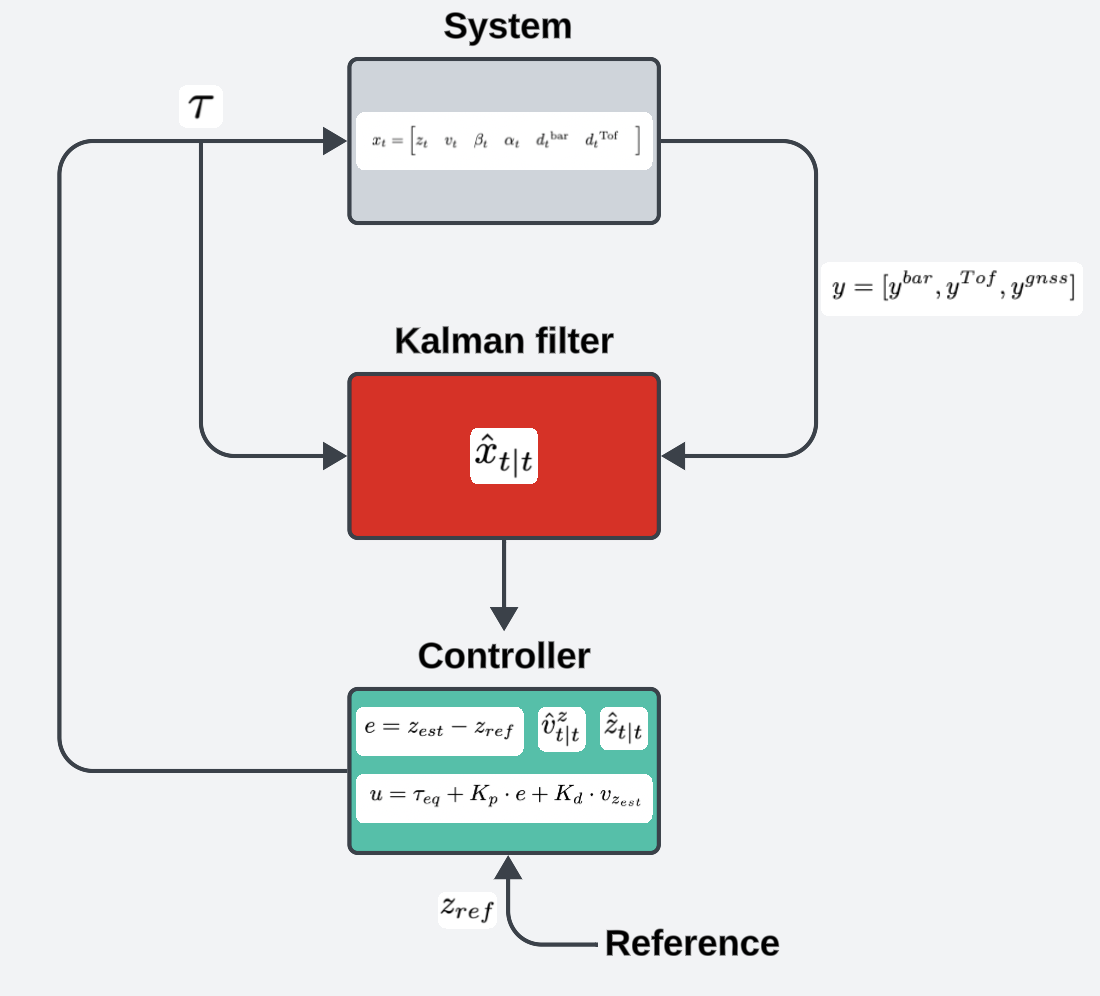
\includegraphics[width=0.8\textwidth]{Pictures/PD_controller_flowchart.png}
  \caption{Alitiude control system flowchart}
  \label{fig:PD_controller_flowchart}
\end{figure}

As seen in the flowchart above in Figure:\ref{fig:PD_controller_flowchart} the system starts by defining the state estimate (\(x_t\)) whitch then defines the output (\(y = [y^{bar}, y^{ToF}, y^{gnss}]\)). The Kalman filter then usesthe measurements y to update updates the state estimate (\(\hat{x}_{t|t}\)) where the controller uses the updated altitude (\(\hat{z}_{t|t}\)) to determine the error (\(e\)) by subtracting the currect estimated altitude (\(z_{est}\)) from the inputed refferance altitude(\(z_{ref}\)). The PD controller then takes the pre defined throttle equilibrium (\(\tau_{eq}\)) and updated estimated vertical velocity (\(\hat{v}^z_{t|t}\)), computes a new throttle command \(u\) to adjust the altitude of the quadcopter.

\subsection{Simulations}\label{PD_simulations} In the world of autonomous
systems, behaviour prediction and control accuracy is critical, especially for
systems with complicated dynamics like quadcopters. At the heart of this
endeavour are simulations, which provide a flexible and perceptive environment
for algorithm creation and validation. This section explores the extensive
simulation environment that was meticulously developed to evaluate and improve
the two essential parts of our control system: the proportional-derivative (PD)
controller and the Kalman filter.

Accross all simulations, Proportional Gain, Derivative Gain and Equilibrium
Throttle are all set to the values denoted above, Section:\ref{PD_control}

The process noise covariance matrix \( Q \) is given by:
\begin{equation}
Q = \begin{bmatrix}
0.001^2 & 0 & 0 & 0 & 0 & 0 \\
0 & 0.01^2 & 0 & 0 & 0 & 0 \\
0 & 0 & (0.1 (2.77 \times 10^{-6}))^2 & 0 & 0 & 0 \\
0 & 0 & 0 & (0.1 (1.74 \times 10^{-7}))^2 & 0 & 0 \\
0 & 0 & 0 & 0 & 0.50^2 & 0 \\
0 & 0 & 0 & 0 & 0 & 0.10^2 \\
\end{bmatrix}
\end{equation}
Where, \( \sigma_z, \sigma_v, \sigma_\alpha, \sigma_\beta \) are 0.001, 0.01, \(
2.77 \times 10^{-6} \), and \( 1.74 \times 10^{-7} \), respectively.
\bigskip

The measurement noise covariance matrix \( R \) is defined as:
\begin{equation}
R = \begin{bmatrix}
(0.25(0.1))^2 & 0 & 0 \\
0 & (0.075(0.1))^2 & 0 \\
0 & 0 & (0.01(0.1))^2 \\
\end{bmatrix}
\end{equation}
Where, \( \sigma_{\text{bar}}, \sigma_{\text{gnss}}, \sigma_{\text{ToF}} \) are
\( 0.25 \times T_s \), \( 0.075 \times T_s \), and \( 0.01 \times T_s \)
respectively.

\subsubsection*{Both \(\alpha\) and \(\beta\) are estimated}
In the fist simulation \(\alpha\) and \(\beta\) along with the Time of Flight
bias (\(d^{ToF}\)), Barometer bias (\(d^{bar}\)), altitude velocity and throttle
reference are being predicted.
\begin{figure}[H]
  \centering
  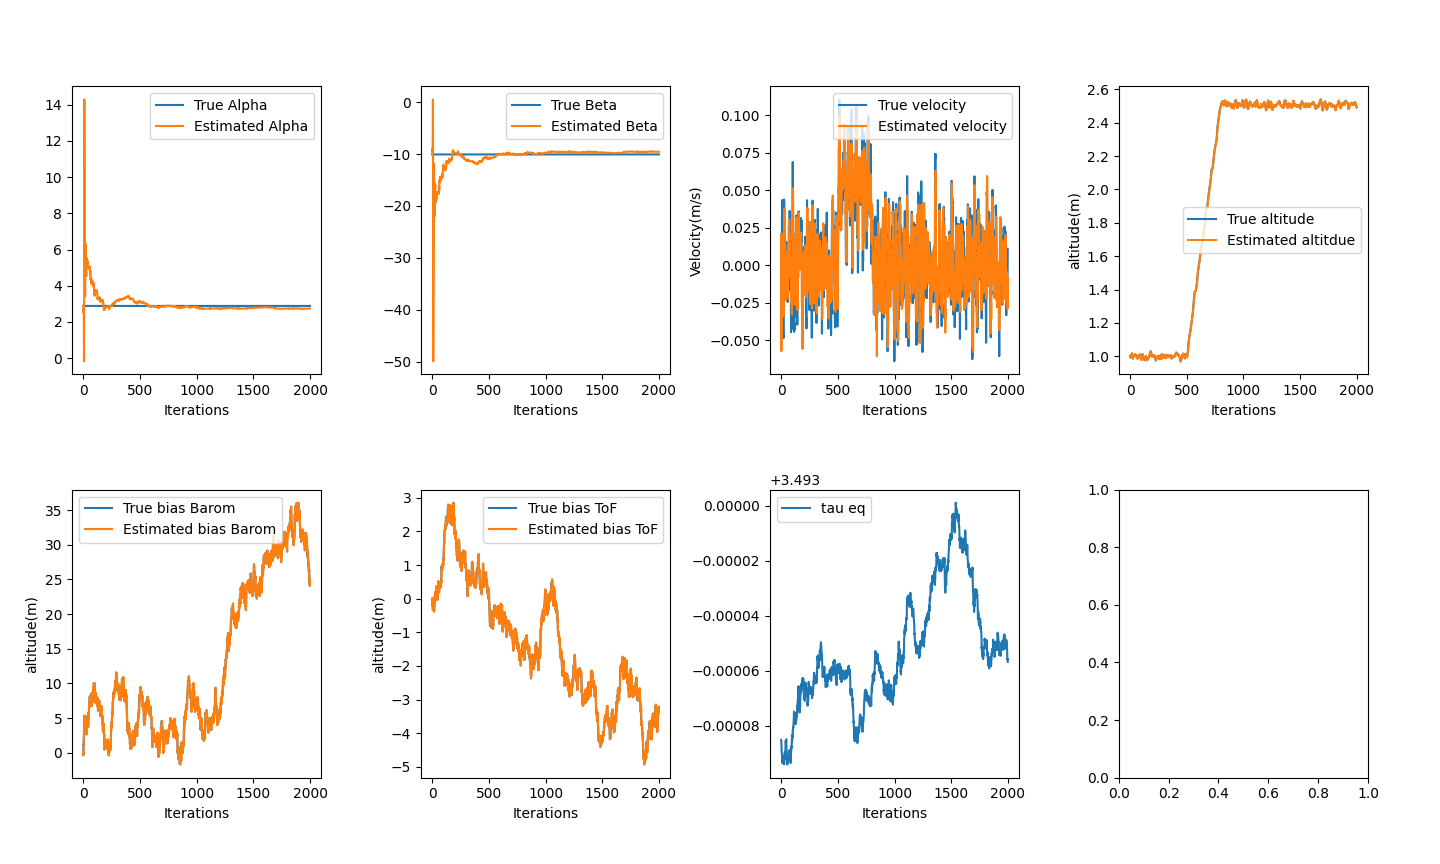
\includegraphics[width=0.9\textwidth]{Pictures/no_constant_PD.png}
  \caption{Simulation1: Both alpha and beta being predicted}
  \label{fig:no_constant_PD}
\end{figure}
In this simulation the quadcopters altitude control system's performance is
evaluated. The system uses a Kalman filter for state estimation, tackling noise
and sensor bias and a PD controller for altitude adjustments.

Observations from the simulation after processing 2000 time steps, with a
sampling time \(T_s\) of 0.1 seconds, reveal several key dynamics;

The Kalman filter’s ability to estimate values of \(\alpha\) and \(\beta\),
which relate throttle input to lifting as well as for \((d^{ToF})\) and
\((d^{bar})\) in meters for the Time of flight and Barometer sensors
respectively is clearly visible within this simulation. The estimated values for
each do indeed converge in on the true values. This is a clear indication of the
kalman filter’s ability to conduct real-time estimation of the values even when
system and measurement noise are present.

Beginning at a reference altitude of 0.5 meters, the quadcopters altitude begins
to increase after the 500th time step to the 800th, due to the reference
altitude being increased between these times. In response to this change the
throttle reference \((\tau)\) is changed by the PD controller. The real and
estimated altitudes suggest a controlled climb during this period, showing that
the system has effectively guided the quadcopter to the new reference point
using a PD controller.

The velocity graph showcases the control systems dynamic response to this change
in altitude. As seen the velocity changes in-line with the altitude changes,
this indicates that the PD controllers ability to change the quadcopters speed
to achieve and sustain the target altitude has been well implemented.

The throttle reference graph denoted by \(\tau\) shows that the PD controller
actively changes the throttle input in response to the new change in reference
altitude. Once the altitude reference levels off after timestep 800 the throttle
input begins to stabilise, indicating that the controller is reaching a new
equilibrium point.
 
A well-tuned PD controller is shown by the system's minimum overshoot and smooth
approach to the new altitude reference. The derivative component effectively
dampens any oscillations, contributing to a swift yet stable climb to the
desired altitude.

in conclusion, this simulation shows how the PD controller designed used in
tandem with the Kalman filter may be used to successfully manage altitude in the
quadcopter. The Controller adjusts the reference altitude and responds well to
the changes posed on the quadcopter. The controller runs with precise state
information thanks to the Kalman filter's skilful tracking and estimation of
critical system parameters and sensor biases, making this a viable solution for
altitude control in the real quadcopter.



\subsubsection*{\(\alpha\) is constant whilst \(\beta\) is being estimated}
In the second simulation \(\alpha\) is set at as a constant and \(\beta\) is
estimated along with the Time of Flight bias (\(d^{ToF}\)), Barometer bias
(\(d^{bar}\)), altitude velocity and throttle reference are being predicted.
\begin{figure}[H]
  \centering
  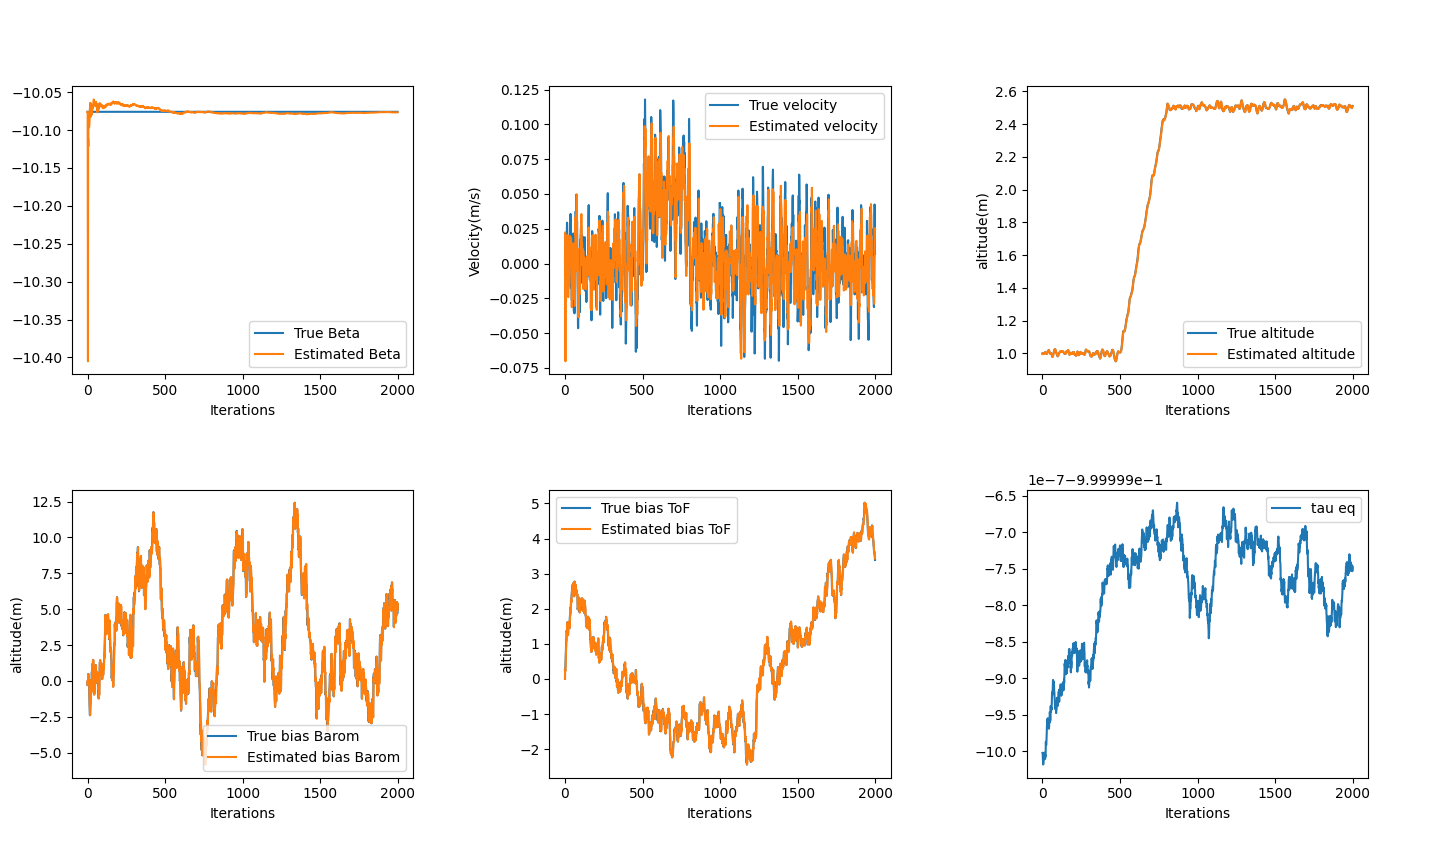
\includegraphics[width=0.9\textwidth]{Pictures/a_constant_PD.png}
  \caption{Simulation2: constant alpha and beta being predicted}
  \label{fig:a_constant_PD}
\end{figure}
In this simulation the quadcopters altitude control system's performance is
evaluated. The system uses a Kalman filter for state estimation, tackling noise
and sensor bias and a PD controller for altitude adjustments.

Observations from the simulation above Figure:\ref{fig:a_constant_PD} after
processing 2000 time steps, with a sampling time \(T_s\) of 0.1 seconds, reveal
several key dynamics;

The kalman filter’s ability to estimate values of \(\beta\), as well as for
\(d^{ToF}\) and \(d^{bar}\) in meters for the Time of flight and Barometer
sensors respectively is clearly visible within this simulation, notably when
compared to the simulation above (Figure:\ref{fig:no_constant_PD}) \(\alpha\) is
no longer being estimated. The estimated values for each do indeed converge in
on the true values. This is a clear indication of the kalman filter’s ability to
conduct real-time estimation of the values even when system and measurement
noise are present.

Beginning at a reference altitude of 0.5 meters, the quadcopters altitude begins
to increase after the 500th time step to the 800th, due to the reference
altitude being increased between these times. In response to this change the
throttle reference \((\tau)\) is changed by the PD controller. The real and
estimated altitudes suggest a controlled climb during this period, showing that
the system has effectively guided the quadcopter to the new reference point
using a PD controller.

The velocity graph again showcases the control systems dynamic response to this
change in altitude. As seen the velocity changes in-line with the altitude
changes, this indicates that the PD controllers ability to change the
quadcopters speed to achieve and sustain the target altitude has been well
implemented.

The throttle reference graph denoted by \(\tau\) shows that the PD controller
actively changes the throttle input in response to the new change in reference
altitude. Once the altitude reference levels off after time-step 800 the throttle
input begins to stabilise, indicating that the controller is reaching a new
equilibrium point.
 
A well-tuned PD controller is shown by the system's minimum overshoot and smooth
approach to the new altitude reference. The derivative component effectively
dampens any oscillations, contributing to a swift yet stable climb to the
desired altitude.

in conclusion, this simulation shows how the PD controller designed used in
tandem with the Kalman filter may be used to successfully manage altitude in the
quadcopter. While alpha is considered a constant in this scenario, not subject
to estimation by the Kalman filter, the system's performance remains robust. The
Controller adjusts the reference altitude and responds well to the changes posed
on the quadcopter. The controller runs with precise state information thanks to
the Kalman filter's skilful tracking and estimation of critical system
parameters and sensor biases, making this a viable solution for altitude control
in the real quadcopter.


\subsubsection*{\(\beta\) is constant whilst \(\alpha\) is being estimated}
In the third simulation \(\beta\) is set at as a constant and \(\alpha\) is
estimated along with the Time of Flight bias (\(d^{ToF}\)), Barometer bias
(\(d^{bar}\)), altitude velocity and throttle reference are being predicted.
\begin{figure}[H]
  \centering
  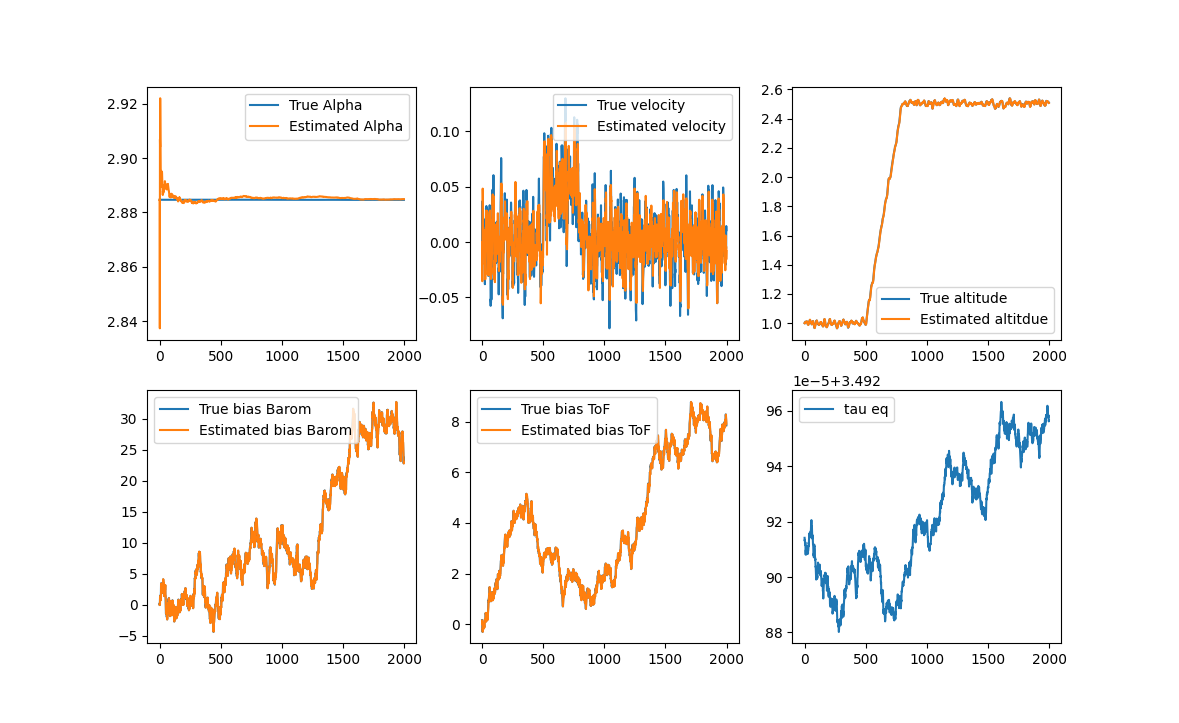
\includegraphics[width=0.9\textwidth]{Pictures/b_constant_PD.png}
  \caption{Simulation3: constant beta and alpha being predicted}
  \label{fig:b_constant_PD}
\end{figure}
In this simulation the quadcopters altitude control system's performance is
evaluated. The system uses a Kalman filter for state estimation, tackling noise
and sensor bias and a PD controller for altitude adjustments.

Observations from the simulation above Figure:\ref{fig:b_constant_PD} after
processing 2000 time steps, with a sampling time \(T_s\) of 0.1 seconds, reveal
several key dynamics;

The kalman filter’s ability to estimate values of \(\alpha\), as well as for
\(d^{ToF}\) and \(d^{bar}\) in meters for the Time of flight and Barometer
sensors respectively is clearly visible within this simulation, notably when
compared to the simulation above (Figure:\ref{fig:no_constant_PD}) \(\beta\) is
no longer being estimated. The estimated values for each do indeed converge in
on the true values. This is a clear indication of the kalman filter’s ability to
conduct real-time estimation of the values even when system and measurement
noise are present.

Beginning at a reference altitude of 0.5 meters, the quadcopters altitude begins
to increase after the 500th time step to the 800th, due to the reference
altitude being increased between these times. In response to this change the
throttle reference \((\tau)\) is changed by the PD controller. The real and
estimated altitudes suggest a controlled climb during this period, showing that
the system has effectively guided the quadcopter to the new reference point
using a PD controller.

The velocity graph again showcases the control systems dynamic response to this
change in altitude. As seen the velocity changes in-line with the altitude
changes, this indicates that the PD controllers ability to change the
quadcopters speed to achieve and sustain the target altitude has been well
implemented.

The throttle reference graph denoted by \(\tau\) shows that the PD controller
actively changes the throttle input in response to the new change in reference
altitude. Once the altitude reference levels off after time-step 800 the throttle
input begins to stabilise, indicating that the controller is reaching a new
equilibrium point.
 
A well-tuned PD controller is shown by the system's minimum overshoot and smooth
approach to the new altitude reference. The derivative component effectively
dampens any oscillations, contributing to a swift yet stable climb to the
desired altitude.

in conclusion, this simulation shows how the PD controller designed used in
tandem with the Kalman filter may be used to successfully manage altitude in the
quadcopter. While \(\beta\) is considered a constant in this scenario, not
subject to estimation by the Kalman filter, the system's performance remains
robust. The Controller adjusts the reference altitude and responds well to the
changes posed on the quadcopter. The controller runs with precise state
information thanks to the Kalman filter's skilful tracking and estimation of
critical system parameters and sensor biases, making this a viable solution for
altitude control in the real quadcopter.


\subsubsection*{Simulations conclusion}
In conclusion, the simulation where both \(\alpha\) and \(\beta\) were being
estimated shown in Figure:\ref{fig:no_constant_PD} has shown notable
effectiveness. The Kalman filters ability to estimate values in real time,
allowing them to converge quickly on there real values should not go un noted.
The accurate estimation of the Kalman filter forms the basis for the
Proportional Derivative (PD) controllers ensuring its responses are reliable on
data.

The Kalman filters efficiency is evident in this simulation, despite requiring
estimation for both \(\alpha\) and \(\beta\) the system still displays a good
degree of stability and control. The PD controller allows the system to respond
to a changing reference altitude without any oscillations. This suggests that
the inclusion of \(\alpha\) and \(\beta\) has not negatively impacted the
systems performance when coparing the results from the other two simulations in
figures:\ref{fig:a_constant_PD} and \ref{fig:b_constant_PD}.

The results show that the decision to estimate both alpha and beta within the
Kalman filter formulation for sensor fusion of altitude sensors in the system,
is promising. This system, when designed and implemented in the quadcopter using
a PD controller, can not only maintain the altitude accurately but also respond
smoothly and seamlessly in the event of any changes in the reference altitude.
It is the combination of all the elements of the system that make it a feasible
option for real-life use. The entire proposition offers a high level of fine
control that is not only ideal but also essential for autonomous quadcopter
flight.

\section{Position control (not yet implemented)}
The incorporation of an advanced position control system is critical for
optimising the quadcopter's performance and stability, especially in dynamic
conditions. This system makes use of the accuracy and dependability of the
onboard GNSS module and works in conjunction with the altitude control mechanism
described in Section:\ref{Altitude_control}. The GNSS module provides essential
latitude and longitude data that establishes the groundwork for real-time
position control.

When the system is activated by, toggling switch C to its range-2 position as
described in Section:\ref{radio}, it instantly locks in the altitude and current
coordinates as the reference points. This critical point initiates highly
responsive control loops in which these reference values serve as the basis for
the navigation and stabilisation tasks that follow.

With these reference points in mind, the control system uses a
Proportional-Derivative (PD) controller, which is explained in detail in
Section:\ref{PD_control}, to carefully control altitude. By doing this, the
quadcopter is guaranteed to keep a constant elevation, which is essential for
efficient position control. In addition, the quadcopter's movement is controlled
across all axes not just the z-axis by incorporating a
Proportional-Integral-Derivative (PID) controller, which is covered in more
detail in Section:\ref{PID_control}. A harmonious balance between location
precision and altitude stability is ensured by this dual-controller approach. 

The quadcopter should hover with high accuracy because of the smooth integration
of various control mechanisms. The system can instantly make modifications by
continuously comparing the current positioning data with the predefined
reference points. This degree of responsiveness is essential for adjusting to
outside factors like wind currents and making sure the quadcopter's position is
unaffected by them.

Furthermore, new applications where accuracy and stability are critical, such as
autonomous navigation, search and rescue, aerial photography, are made possible
by this sophisticated position control system.

\subsection{Global positioning to Local positioning}\label{gp_vs_lp}
In order for the system to be able to read the reference points accurately, conversion from global position to local position will be needed.

Global positioning refers to its location on a given coordinate system such as GNSS module latitude and longitude. There values are useful when attempting to find the Quadcopters position on a global scale. For our use a better approach is having a local position relative to a given standpoint or start point.

By ustilising the base station in Section:\ref{fig:gnss_base_station} coordinates of the rover module can be parsed relitive to the base station in a local frame along a 2D plane.

First the quadcopters Global coordinates (latitude,longitude and altitude) are converted to the ECEF coordinate system. This system represents points with Cartesian coordinates (x, y, z) with the origin at the center of the Earth.

next the ECEF coordinates will be translated into a north, east down system, using a rotation matrix that accounts for the orientation of the Earth's surface at the base station relitive to the rover module. 

Below, you can view graphs that depict the rotational differences along an axis between local and global positioning systems.

\begin{figure}[H]
  \begin{minipage}{0.5\textwidth}
    \centering
    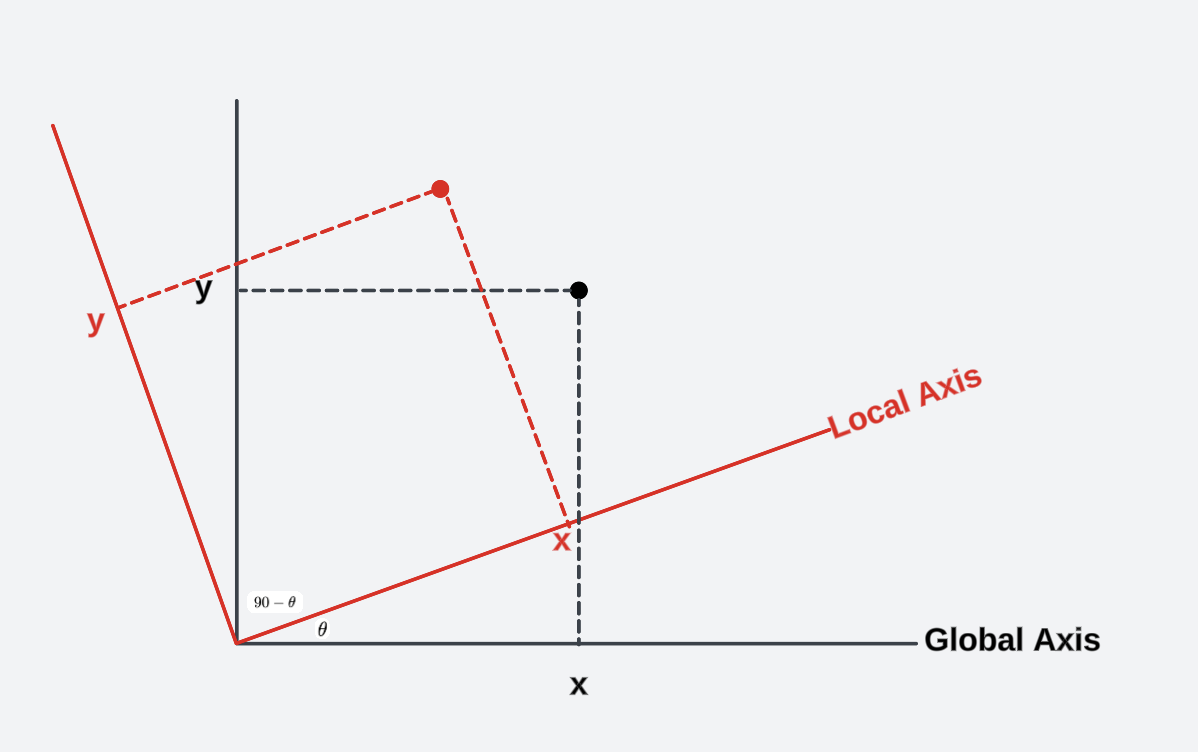
\includegraphics[width=0.9\textwidth]{Pictures/local_vs_global_1.png}
    \caption{Graph representing the difference\\ between global and and local positioning }
    \label{fig:local_vs_global_1}
  \end{minipage}
  \begin{minipage}{0.5\textwidth}
    \centering
    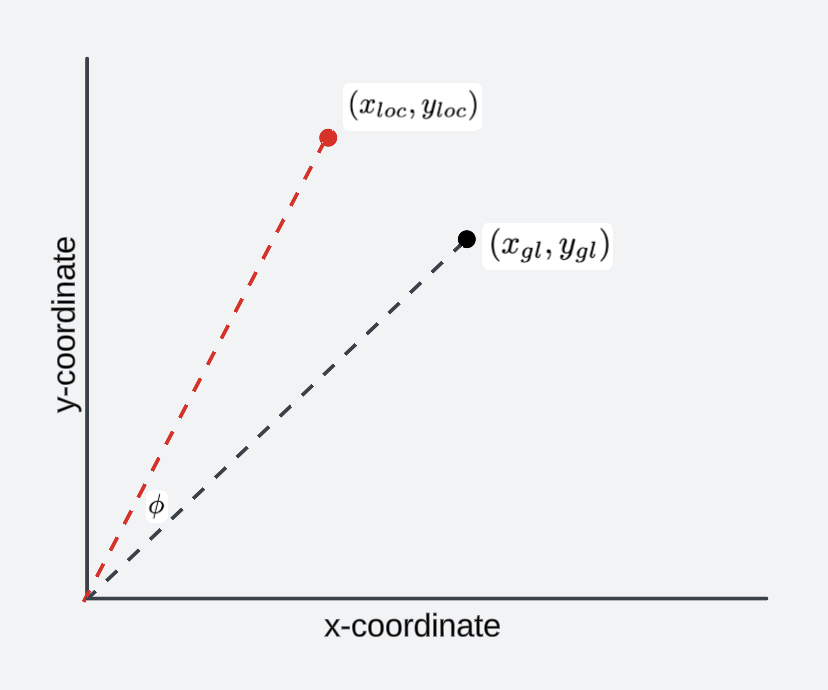
\includegraphics[width=0.7\textwidth]{Pictures/local_vs_global_2.png}
    \caption{Global vs Local position}
    \label{fig:local_vs_global_2}
  \end{minipage}
\end{figure}

In order to find the local x and y coordinates denoted by \(x_{loc}, y_{loc}\) in Figure:\ref{fig:local_vs_global_2} a rotation matrix is used in the following equation. 

\begin{equation}
  \begin{bmatrix}
    x_{loc}\\
    y_{loc}
  \end{bmatrix}
  =
  \begin{bmatrix}
    cos\phi & -sin\phi\\
    sin\phi & cos\phi
  \end{bmatrix}
  \begin{bmatrix}
    x_{gl}\\
    y_{gl}
  \end{bmatrix}
\end{equation}

where, \(\phi\) represents the heading taken from the compass in the IMU

\subsection{Modelling}
The model used for Position control can be defined as,
\begin{itemize}
  \item \textbf{Position Update:}
  \[
  p_{t+1} = p_t + T \cdot v_t
  \]
  
  \item \textbf{Velocity Update:}
  \[
  v_{t+1} = v_t + T \left( R(\theta^r_t, \theta^p_t) \begin{bmatrix}0 \\ 0 \\ \dot{z}_t\end{bmatrix} + \begin{bmatrix}0 \\ 0 \\ -g\end{bmatrix} - \begin{bmatrix}A^x & 0 & 0 \\ 0 & A^y & 0 \\ 0 & 0 & A^z\end{bmatrix} v_t \right)
  \]
  
  \item \textbf{Attitude Update for Roll and Pitch:}
  \[
  \theta^r_{t+1} = \theta^r_t + \frac{T}{\omega^r}(K^r\theta^{r,ref}_t - \theta^r_t)
  \]
  \[
  \theta^p_{t+1} = \theta^p_t + \frac{T}{\omega^p}(K^p\theta^{p,ref}_t - \theta^p_t)
  \]
  \end{itemize}
  

where \(p_t = (p^x_t, p^y_t, p^z_t)\) and \(v_t\) are the position and velocity of the quadcopter in the global frame of refferance. \(\theta^p\) and \(\theta^r\) are the pitch and roll angles. \(\theta^{p,ref}\) and \(\theta^{r,ref}\) are the pitch and roll refferances that are sent to the controller. \(\dot{z}_t\) is the vertical acceleration in the z-axis as defined in \ref{vertical acceleration}, while \(A^x, A^y, A^z\) are the linear drag coefficients. \(T\) is the sampeling time.

The attitde control system is then moddled, time constants \(\omega^p\) and \(\omega^r\) and gains \(K^r\) and \(K^p\)
for the roll and pitch. 

Finally \(R(\theta^r, \theta^p)\) can be defined as eular angles in rotation matrix form as

\begin{equation}
  R(\theta^r, \theta^p) = R^y(\theta^p)R^x(\theta^r)
\end{equation}

where, 
\begin{align}
  R^x(\theta^r) &= \begin{bmatrix}
  1 & 0 & 0 \\
  0 & \cos(\theta^r) & -\sin(\theta^r) \\
  0 & \sin(\theta^r) & \cos(\theta^r)
  \end{bmatrix}, \\
  R^y(\theta^p) &= \begin{bmatrix}
  \cos(\theta^p) & 0 & \sin(\theta^p)\\
  0 & 1 & 0 \\
  -\sin(\theta^p) & 0 & \cos(\theta^p)
  \end{bmatrix}
\end{align}

These equations were derived and changed from \cite{positionControl}

\subsection{PID control}\label{PID_control} In order to utilise position
control on the quadcopter PID (Proportional-integral-Derivative) controller's
have been used, one for latitude \((y_gl)\) control and the other for longitude \((x_gl)\) control. A
PID controller is a control loop feedback mechanism which is widely used in
industrial control systems. It is a type of linear feedback control system that
combines three kinds of control:
\begin{itemize}
  \item \textbf{Proportional control(P)}: This part of the algorithm reacts to
  the current error, which is the difference between the set point and the
  processes current value. The proportional term analyses the error and produces
  a linear output based on the error. This results in the rapid response of the
  system to deviations from the desired setpoint, helping to stabilize the
  system by moving the process variable in the right direction. The Proportional
  gain is a variable parameter that sets the level of aggression of the PID
  controller in its response to error. A high Kp will means a larger output for
  a given error – and, therefore, a faster response of the system to make up for
  the error – but setting Kp too high will lead to instability in the form of
  gross oscillations about the setpoint.
  \item \textbf{Integral (I)}: The integral control deals with the accumulated
  error over time by emphasising the difference between the system's actual
  performance and the planned reference setpoint. The integral term adds up
  previous errors, supplying a corrective force proportionate to the length and
  size of the deviation, in contrast to the proportional component, which just
  reacts to the current error. This feature of the controller ensures that the
  process variable finally converges to the setpoint and is especially useful at
  removing steady-state faults. The controller's sensitivity to the cumulative
  mistake is controlled by the Integral gain, or Ki. A well adjusted Ki can
  minimise offset considerably, but an overly high value could cause
  oscillations and overshooting, which would compromise the stability of the
  system.
  \item \textbf{Derivative(D)}: The derivative term in a PD controller plays a
  crucial role in forecasting the system's future dynamics based on the current
  rate at which the error is changing. It acts as a form of predictive control,
  providing a damping force that enhances the stability of the system. By
  tempering the response generated by the proportional component, the derivative
  action effectively mitigates overshoot—preventing the system output from
  exceeding the desired setpoint. Increasing the derivative time (Kd) parameter
  will cause the control system to react strongly to changes in the error term
  and will increase the speed of the overall control system response. Moreover,
  it contributes to a faster response by reducing the settling time, which is
  the time it takes for the system to stabilize within a certain range of the
  setpoint.
\end{itemize}
generally a PID controller is given by the following equation: 

\begin{equation}
  u(t) = K_p e(t) + K_i \int_{0}^{t} e(\tau) \, d\tau + K_d \frac{d}{dt} e(t)
\end{equation}
where:
\begin{itemize}
    \item $u(t)$ is the controller output at time $t$.
    \item $e(t)$ is the error between the setpoint and the process variable at
    time $t$.
    \item $K_p$ is the proportional gain, a tuning parameter that scales the
    magnitude of the proportional term.
    \item $K_i$ is the Integral gain, a tuning parameter that determines the
    reaction based on the sum of recent errors, providing a correction based on
    the historical cumulative error, which helps eliminate steady-state error.
    \item $K_d$ is the derivative gain, a tuning parameter that scales the
    magnitude of the derivative term.
    \item $\int_{0}^{t} e(\tau) \, d\tau$ represents the Integral of the error
    over time from 0 to the current time $t$, accounting for the accumulation of
    past errors.
    \item $\frac{d}{dt} e(t)$ is the rate of change of the error (derivative of
    the error with respect to time)
\end{itemize}
\subsubsection*{Implementation}
In order to implement Position control in the quadcopter two PID controllers
need to be utilised, one for control of the latitude data and the other for
longitude data. 

In order to calculate the position error (e) the difference between the current
position and the reference position must be calculated. For both latitude, longitude and altitude controllers the equations would look like this, where x represents
longitude, y represents latitude and z is the altitude in local format(Section:\ref{gp_vs_lp}):
\begin{align}
  e_{\text{x}} =&  x_{\text{current}} - x_{\text{ref}}
  \\
  e_{\text{y}} =&  y_{\text{current}} - y_{\text{ref}}
  \\
  e_{\text{z}} =&  z_{\text{current}} - z_{\text{ref}}
\end{align}
The control action (u) is the sum of three terms: the baseline control
inputs\((u_{\text{baseline}})\), the proportional term, the integral term and
the derivative term. The proportional term is the product of the proportional
gain (Kp) and the altitude error. The integral term is the product of the
integral gain(Ki) and the position errors over time. The derivative term is the
product of the derivative gain (Kd) and the rate of change in error.

The continuous-time pitch control equation, where \( \theta^p \) represents the pitch angle and \( v_x \) is the velocity along the \(x\) axis, is given by:

\begin{equation}
  \theta^{p,\text{ref}}_t = K_{p,x} \cdot e_x + K_{i,x} \cdot \sum e_x \Delta t + K_{d,x} \cdot v_x
\end{equation}

Similarly, the roll control equation, where \( \theta^r \) represents the roll angle and \( v_y \) is the velocity along the \(y\) axis, is given by:

\begin{equation}
  \theta^{r,\text{ref}}_t = K_{p,y} \cdot e_y + K_{i,y} \sum e_y \Delta t + K_{d,y} \cdot v_y
\end{equation}

The altitude control equation, where z represents the altitude and v  is the velocity along the z
axis, is given by

\begin{equation}
  u_z = \tau_{eq} + K_{p,z} \cdot e_z + K_{i,z} \sum e_z \Delta t + K_{d,z} \cdot v_z
\end{equation}

where \(\theta_p\)/\(\theta_r\) represents the reference angle that we want to achieve. \(\sum e_y \Delta t\) is the integral of the error over time, which helps in eliminating steady-state errors. \(v_x\)/\(v_y\)/\(v_z\) is the velocity along the specified axis, used for derivative control to anticipate changes in the system.

\subsection{Position control system overview}
\begin{figure}[H]
  \centering
  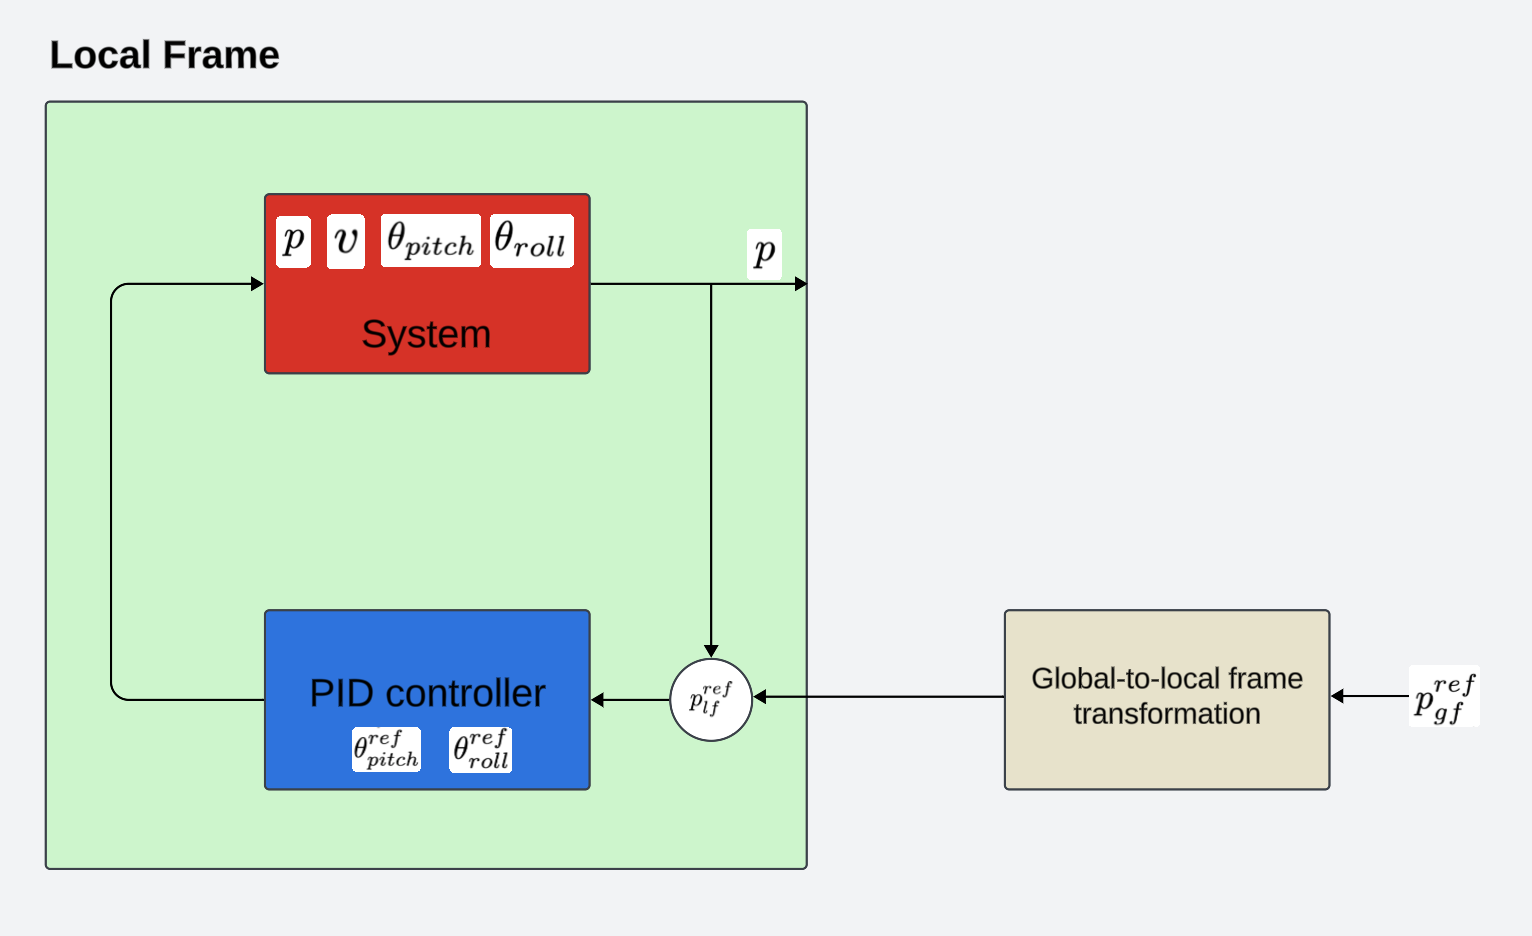
\includegraphics[width=0.9\textwidth]{Pictures/position_control_system_flowchart.png}
  \caption{Position control system overview}
  \label{fig:position_control_system_flowchart}
\end{figure}

The flowchart illustrates the position control system within a local frame of reference, the System processes the state variables; the position vector (\(p\)), the velocity vector (\(v\)), and the orientation angles for pitch (\( \theta_{\text{pitch}} \)) and roll (\( \theta_{\text{roll}} \)). The system's output is the current position vector (\(p\)), which serves as an input to the subsequent PID Controller.

The PID controller receives this position vector (\(p\)) and compares it to a local reference position vector (\(p_{\text{lf}}^{\text{ref}} \)), calculating the error (\( e \)). This error, along with the vehicle's current velocity (\(v\)) and a predefined equilibrium thrust (\( T_{\text{eq}} \)), are used to determine the necessary control signals. The reference pitch (\( \theta_{t,\text{ref}}^{\text{pitch}} \)) and roll (\( \theta_{t,\text{ref}}^{\text{roll}} \)) angles are utilized to generate the control signals to correct the vehicle's orientation and maintain its position as well as the updated throttle signal(\(\tau\)).


The \textit{Global-to-local frame transformation} module, takes a reference position in the global frame (\(p_{\text{gf}}^{\text{ref}} \)) and converts it to a corresponding local frame reference position (\(p_{\text{lf}}^{\text{ref}} \)).

The PID controller, which modifies the vehicle’s pitch and roll depending on the transformed reference position, the interaction between these system steps guarantees that the vehicle retains the intended position within the local frame. For the navigation control module in a three-dimensional environment to function accurately and timely, this control loop is indispensable.


\subsection{Simulations}\label{PID_simulations} The accuracy of control
mechanisms is critical in the field of autonomous systems, especially for robots
and drones that have to manoeuvre through challenging settings. The use of
simulations, which provide a flexible and insightful platform for designing and
testing algorithms, is essential to improving these control systems. The purpose
of this simulation environment is to evaluate and improve Position Control with
Proportional-Integral-Derivative controllers. By modifying control inputs in
response to variations between the desired and present positions, PID
controllers play a crucial role in autonomous systems' capacity to achieve
desired position and stability. By using complex simulations, we are able to
precisely adjust the PID parameters to maximise system performance in a variety
of scenarios, guaranteeing accuracy and resilience in the control of
self-governing systems.

Thought the simulations below the PID gains we set are as follows: 

\begin{itemize}
  \item \(K_p\): 2.0
  \item \(K_i\): 0.2
  \item \(K_d\): 0.05
\end{itemize}

\subsection*{Quadcopter manouvering to one waypoint/target point}
\begin{figure}[H]
  \centering
  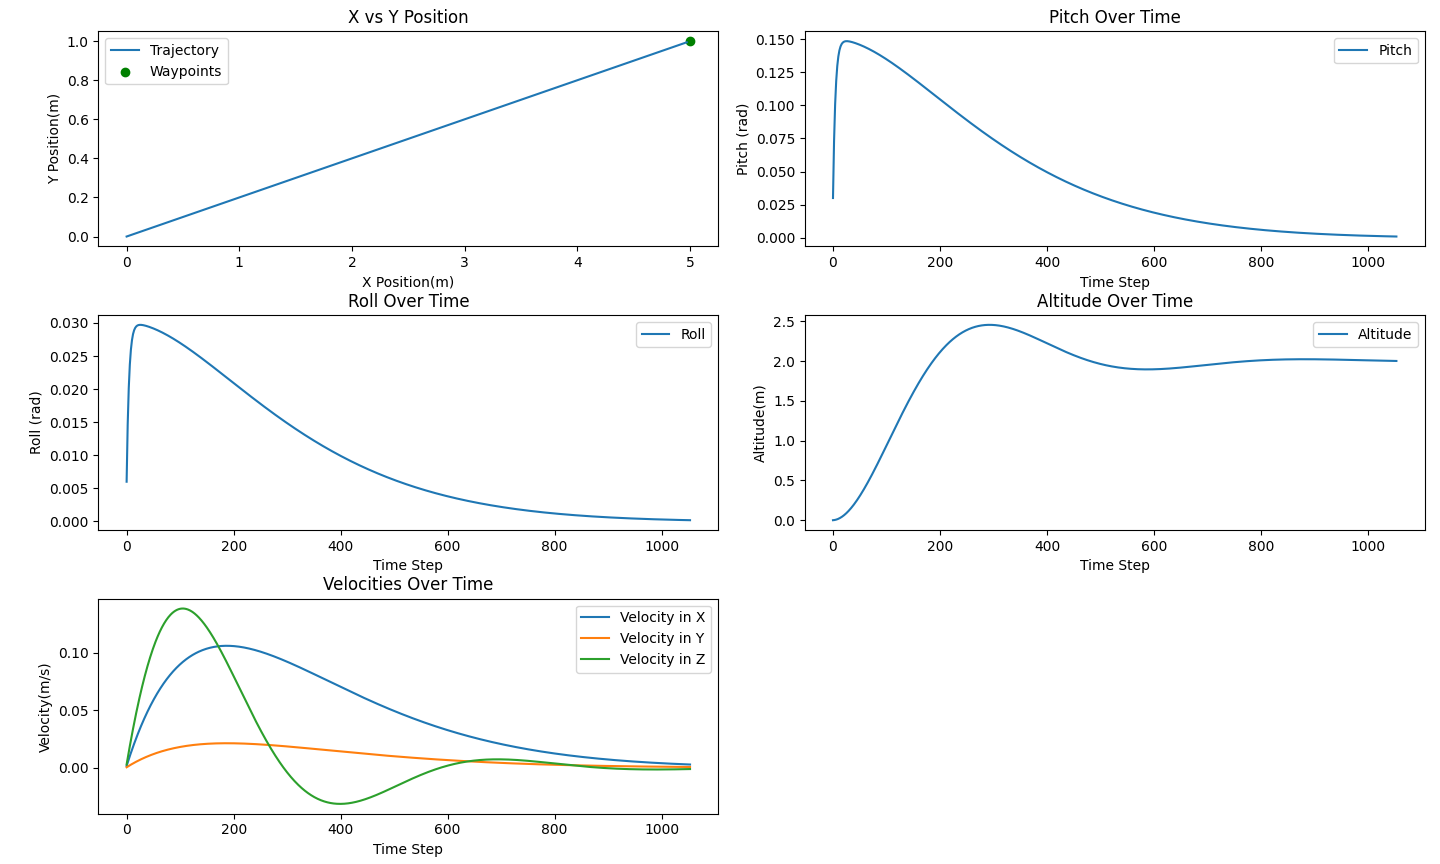
\includegraphics[width=1\textwidth]{Pictures/Position_control_sim.png} 
  \caption{Path of drone from Initial to reference position}
  \label{fig:Drone_path_one_waypoint}
\end{figure}
The quadcopter’s navigation capability is analysed during this advanced
simulation. The quadcopter’s ability to
actively correct is course is made possible by Proportional-Integral-Derivative
(PID) controllers (one for pitch control, one for roll control and one for altitude control).

The x, y and z velocities demonstrate variations in the velocity
chart at the beginning showing a initial strong reaction in both x and z and velocities as a result of the  PID controllers reaction to their larger position error when comparing the current to the refferance position. On the other hand the y velocity doesnt move as fast as its displacement from its target coordinate is not as big. Finally, all velocitys converge on 0 as the quadcopter has reached its desired point.

The quadcopter navigation system is also faced with a difficult dynamic situation, brought about by its target positions location. Both pitch, roll and altitude PID controllers are used simultaneously in this simulation. 

We can see that both pitch and roll alngles are making adjustments in order for the quadcopter to reach its desired target position. It is notable that the roll angle is less than the Pich as it has less distance to travel on the y axis.

Finally, the dones altitude can be seen converging on its target altitude of 2m with a slight overshoot.

In conclusion, the quadcopter PID control systems works well, In was able to reach its desired position with minimal overshoot.This degree of control, which is significant for a number of real-world applications, validates the system's efficacy and dependability and represents a promising standard for durable drone navigation systems.


\subsection*{Quadcopter manouvering around different waypoints}
\begin{figure}[H]
  \centering
  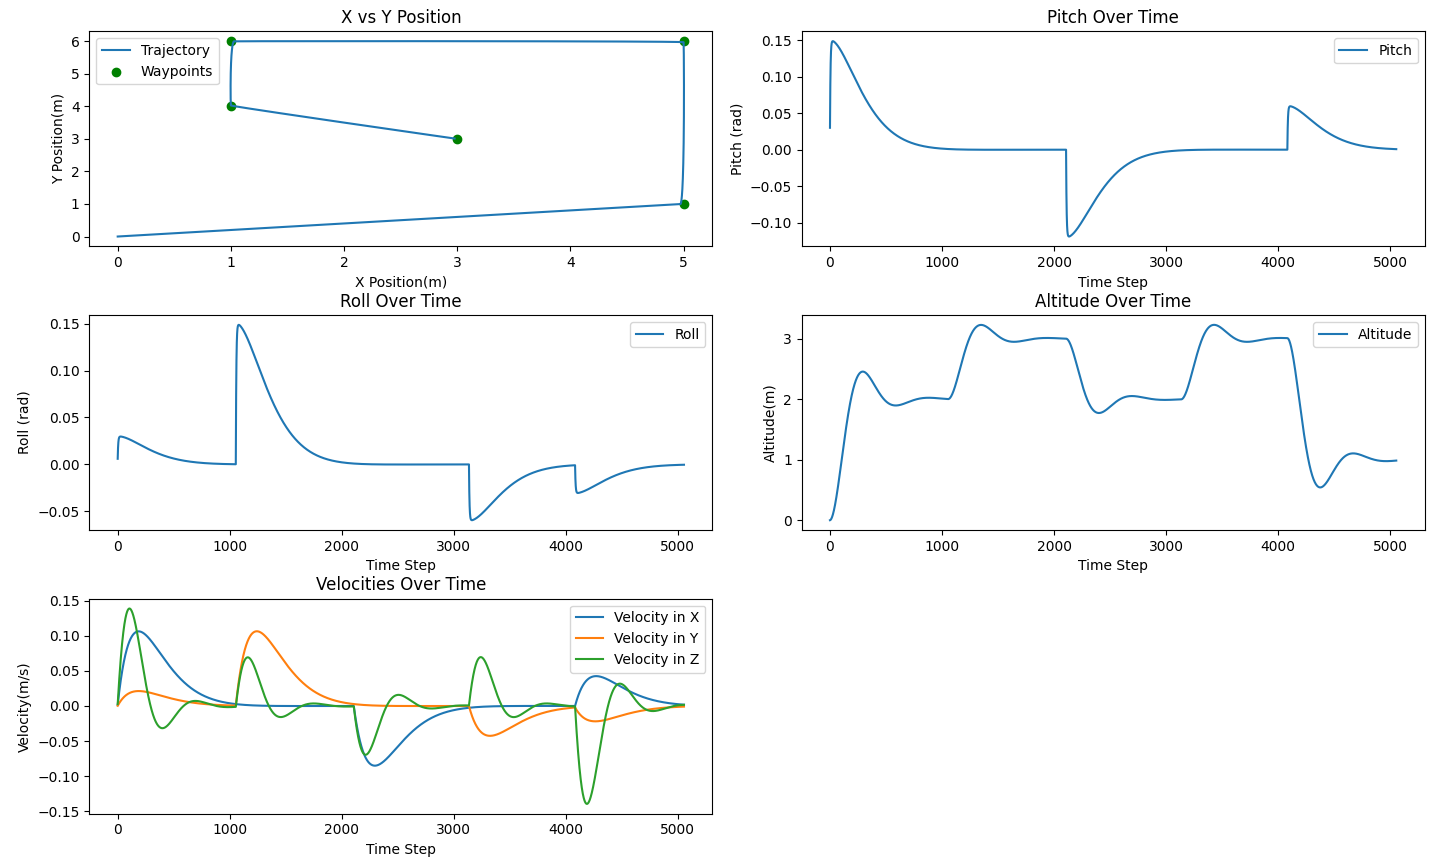
\includegraphics[width=1\textwidth]{Pictures/Position_control_sim_various_waypoints.png} 
  \captionsetup{justification=centering}
  \caption{Path of drone from Initial position around waypoints}
  \label{fig:Drone_path_multiple_waypoints}
\end{figure}
The quadcopter’s navigation capability is analysed during this advanced simulation as it manoeuvres between various different per determined way points. when the quadcopter comes within 3cm from said waypoint it is changed to the next one, and so on.

The quadcopter’s ability to actively correct is course is made possible by Proportional-Integral-Derivative (PID) controllers (one for pitch control, one for roll control and one for altitude) with little to no overshoot when flying between waypoints. The flight course instinctively reacts the changes in waypoints, by adjusting its pitch and roll angles as well asits altitude to travel to the next one. The velocities on the x, y and z axis are ever 
changing and consistantly converging on the desired position.

The quadcopter navigation system is also faced with a difficult dynamic situation, brought about by its everchanging waypoints. Both pitch, roll and altitude PID controllers are used simultaneously in this simulation. 

Finally, the quadcopter PID control systems works well as it moves between waypoints; the results of the simulation exercise indicate high flexibility, accurate results, and stability proving the controllers effectiveness. There is little to no overshoot on when flying between waypoints and all angles and velocities converge on the wapoints. 

\chapter{hardware}\label{hardware}
 This section outlines the various hardware
that is used in forming the overall structure of the quadcopter.

\section{Motors}\label{motors}
\begin{figure}[H]
  \centering
  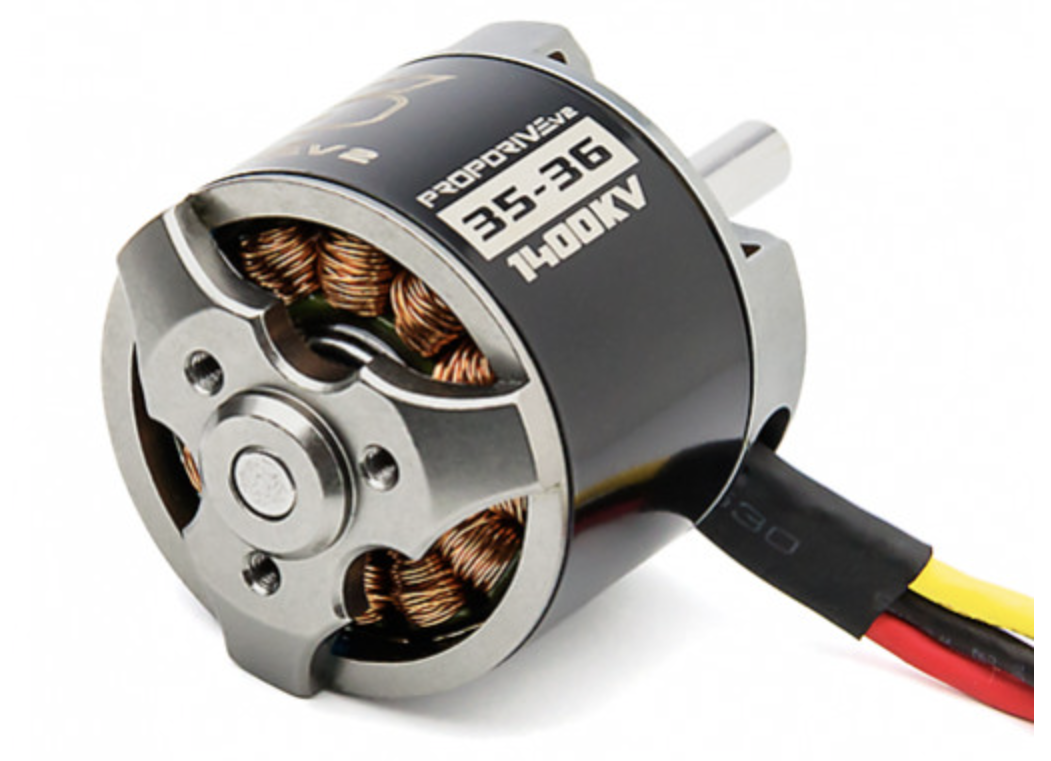
\includegraphics[width=0.3\textwidth]{Pictures/motors.png} 
  \caption{1400KV Brushless Motor}
  \label{fig:motor}
\end{figure}
The PROPDRIVE v2 3536 1400KV Brushless Outrunner Motor is designed to offer
solid performance right out of the box. It features tight windings, smooth
bearings, precision cut stator, and balanced rotors for reliable operation.

Key specifications include its 1400KV (Kilo Volt) rating, meaning that for every
1 Volt applied the motor will turn 1400 times. A maximum current of 45A, and
compatibility with with the Skywalker 50A ESC's which we are using below
(Section:\ref{esc}). The motor is suitable for use with 3-4 cell batteries,
again making it compatible with the 5500mAh 4S 70C LiPo Battery's being used
(Section:\ref{battery}). It has 25mm bolt holes with an M3 bolt thread. It
weighs around 121g and comes with 3.5mm bullet connectors.

\section{Radio}\label{radio}
\begin{figure}[H]
  \centering
  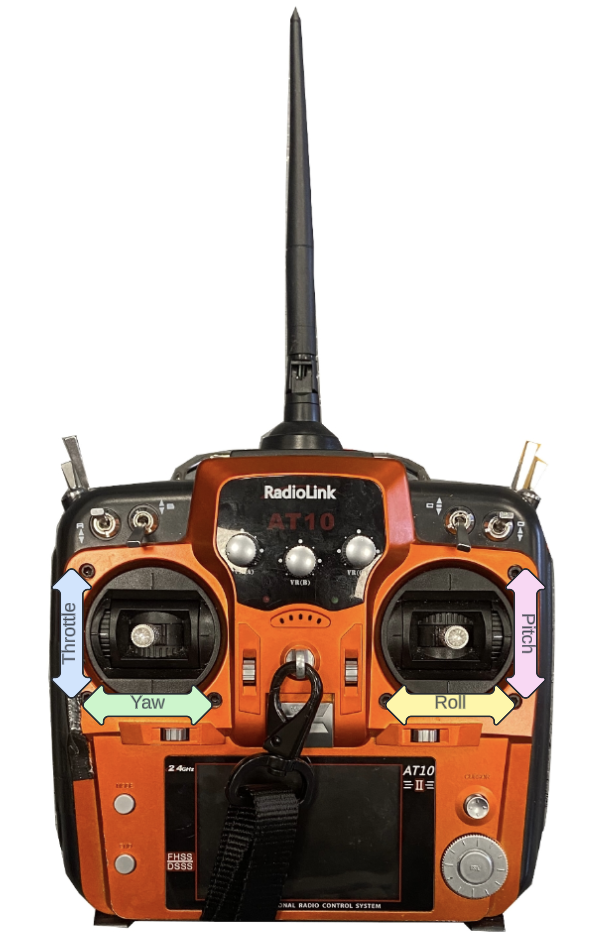
\includegraphics[width=0.4\textwidth]{Pictures/radio.jpg};
  \caption{Radio Controller with Pitch, Roll, Yaw, and Throttle Indicators}
  \label{fig:radio_controller}
\end{figure}
\section{Receiver}
\begin{figure}[H]
  \centering
  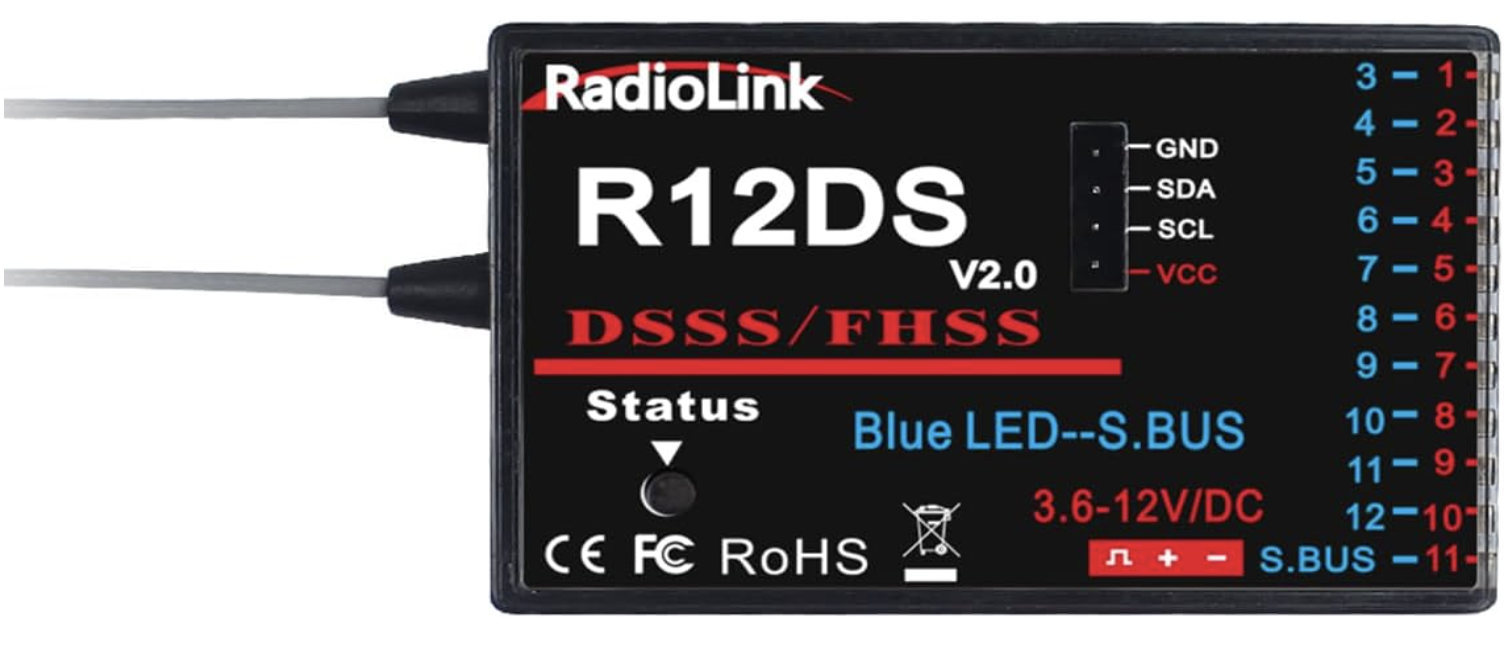
\includegraphics[width=0.3\textwidth]{Pictures/reciever.png}
  \caption{Radiolink R12DS 2.4GHz RC Receiver}
  \label{fig:receiver}
\end{figure}
The radio transmitter and receiver pairs used for this project are the RadioLink
AT10II (Tx) and R12DS (Rx), which are depicted in Figures
\ref{fig:radio_controller} and \ref{fig:receiver}, respectively. At 2.45GHz
bandwidth, the transmitter can deliver data across 12 channels.
Table:\ref{Figure:RC_Controller_Channel_Mapping} presents the channel mapping
for the 12 channels. Consult the instruction manual [...] for details on how to
operate the transmitter.

The SBUS communication protocol is supported by the RadioLink R12DS receiver. In
order to read the data from the 12 radio channels, the receiver is connected to
the Raspberry Pi via SBUS with the aid of the connector. The Raspberry Pi reads
the radio data as a bit-array, and
Table:\ref{Figure:RC_Controller_Channel_Mapping} displays the decoded data
channel and ranges.

\begin{table}[h]
  \centering
  \begin{tabular}{|c|c|c|c|c|}
    \hline
    Channel number/ & Mapping & Signal range & Mapped range & Purpose \\
    data index & & & & \\
    \hline
    0 & Yaw rate & \{300, 1700\}ms & [-3000, 3000]°/s & Yaw rate reference \\
    1 & Pitch & \{300, 1700\}ms & [-30, 30]° & Pitch reference \\
    2 & Throttle & \{300, 1700\}ms & [0, 900]ms & Throttle reference \\
    3 & Roll & \{300, 1700\}ms & [-30, 30]° & Roll reference \\
    4 & Switch C & \{300,1000,1700\}ms & \{0, 1, 2\} & Manual, Altitude Hold,
    Position control \\
    5 & VRA & \{300, 1700\}ms & [0, 1]\% & P Gain (Quaternion Gain) \\
    6 & VRC & \{300, 1700\}ms & [0, 1]\% & D Gain (Angular Velocity Gain) \\
    7 & VRB & \{300, 1700\}ms & [0, 1]\% & (Yaw Angular Velocity Gain)\\
    8 & Switch B & \{300, 1700\}ms & \{False, True\} & Arm \\
    9 & Switch A & \{300, 1700\}ms & \{False, True\} & Save log \\
    10 & Switch D & \{300, 1700\}ms & \{False, True\} & Kill \\
    11 & VRE & \{300, 1700\}ms & [-0.25, 0.25]m & Change Altitude Reference\\
    \hline
  \end{tabular}
  \caption{RC Controller Channel Mapping}
  \label{Figure:RC_Controller_Channel_Mapping}
\end{table}

The physical control sticks, switches, and knobs of the transmitter are
represented as data elements in Table
\ref{Figure:RC_Controller_Channel_Mapping}'s column Mapping. The column labelled
'Channel number' has their matching channel number. The data is sent by the
transmitter in ascending order according to the channel number; that is, the
data packet begins with channel 0 and concludes with channel 11 data.

The receiver reads the data channels beginning with channel 0 and ending with
channel 11. The term 'raw data' is now used to describe this received data. The
column labelled 'Signal range' displays the actual range of the raw data that
was received; the units used are milliseconds. The Raspberry Pi uses SBUS to
read this raw data.

The Raspberry Pi then processes and remaps the raw data to fit the control
algorithm with the aid of a computer programme. The remapped ranges are
displayed in the column Mapped range, and the remapped purpose is displayed in
the Purpose column. The generated references for the attitude controller are the
roll reference, throttle reference, pitch reference, and yaw rate reference in
the Purpose column. To provide the controller commands room, the throttle
reference is set to its maximum at 900 ms.

The ESP32 receives the state of Switch B and Switch D as well as the attitude
reference data. The ESP 32  arms and kills the drone in accordance with the data
from switches B and D. The attitude reference is used by the ESP32's attitude
controller algorithm to determine what control actions are required. In Chapter
\ref{Altitude_control}, the attitude dynamic principles is covered. 

The Raspberry Pi is instructed to save the flight data logs into a
Comma-separated values (CSV) file by means of switch A. Turning switch A on and
off many times will save multiple flight logs in a single flight. It is advised
to land the drone first before storing flight logs.

The switch C is a three-way switch with three states ({0, 1, 2}), and {Manual,
Altitude Hold, position hold} are the mappings for each state. The throttle
signal from the transmitter is sent to the attitude controller while switch C is
in the manual mode and Position hold. Switch C's altitude hold mode activates
the Raspberry Pi's altitude controller and altitude Kalman filter algorithms,
which in turn override the transmitter's throttle reference command. The current
altitude reference is adjusted by ±0.25 metres in altitude hold mode using gain
4. In the position control mode the reference latitude and longitude are
sent to the Raspberry Pi's altitude controller where the PID controller aims to
keep the Quadcopter in the same position.

The trimmers can be used to tune the gains of the control algorithms. When
tuning the attitude controller channel numbers 5, 6, 7 are set to Quaternion
Gain, Angular Velocity Gain and Yaw Angular Velocity Gain respectively (as
denoted by brackets in table:\ref{Figure:RC_Controller_Channel_Mapping}). By
default the trimmers are set to tune the altitude controller with chanel numbers
5 and 6 tuning the P Gain and D Gain ie. $K_{p}$ and ${K}_{d}$ (see
Equation~\ref{PD_controller_eq}) respectively. Furthermore, channel 11 is used
to Change Altitude Reference when in altitude control mode at a max rate of
\unit[4]{cm/s}. 


\section{Flight Controller}\label{flight_controller}
\begin{figure}[H]
  \centering
  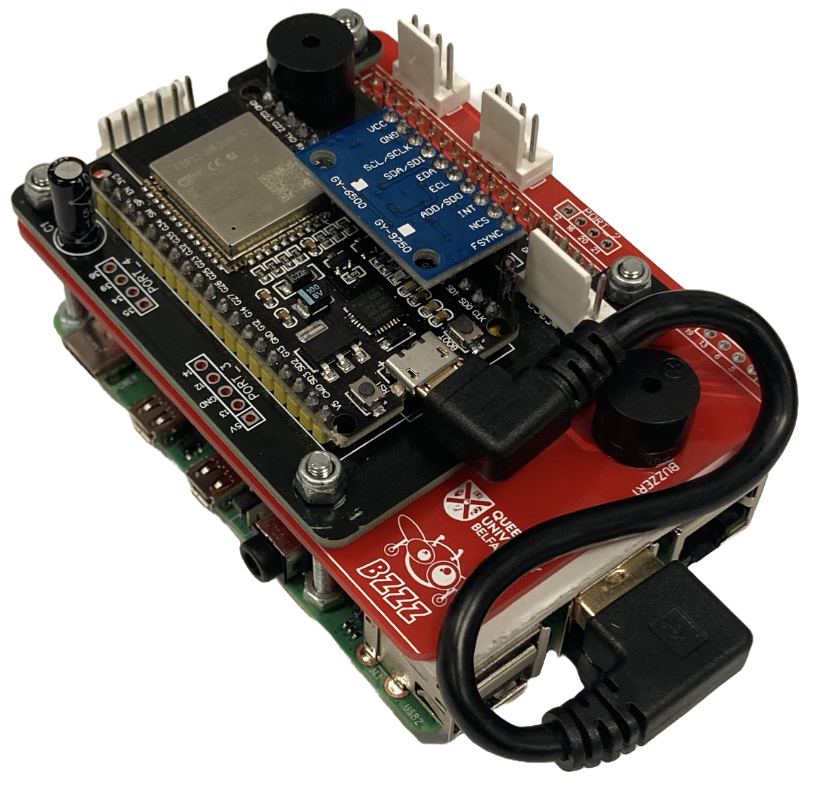
\includegraphics[width=0.35\textwidth]{Pictures/flight_controller.png}
  \caption{Flight controller}
  \label{fig:flightController}
\end{figure}
The flight controller is made up of two main components:
\begin{itemize}
  \item Raspberry Pi
  \item ESP32
\end{itemize}
\subsection{Raspberry Pi}
\begin{figure}[H]
  \centering
  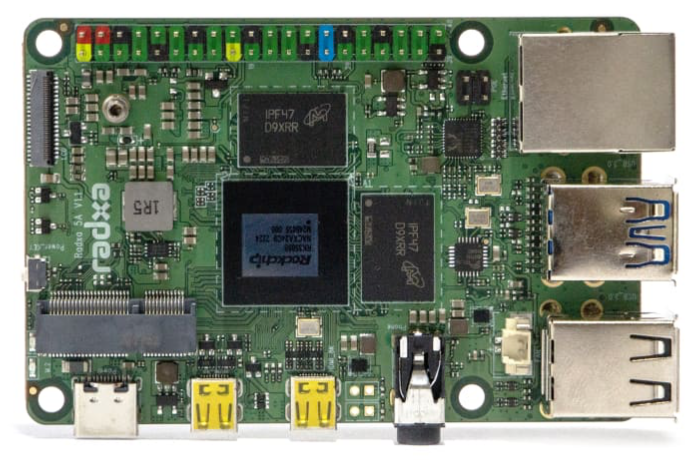
\includegraphics[width=0.3\textwidth]{Pictures/raspberry_pi.png}
  \caption{Raspberry Pi}
  \label{fig:rasberry_pi}  
\end{figure}
The Raspberry Pi is a particularly good option for inclusion into a quadcopter
project because of its powerful processing and multitasking properties. With a
potent quad core Cortex-A72 (ARM v8) 64-bit SoC clocked at 1.5GHz, the Broadcom
BCM2711, the Pi 4B is well-suited to manage intricate calculations and numerous
code executions concurrently. This is critical for a quadcopter, as it handles
multiple tasks at once, including processing real-time sensor data and flying
control algorithms. It is also the perfect brain for a quadcopter because of its
small size, low power consumption, and plenty of GPIO pins for peripheral
connections. This combination enables an aerial platform that is lightweight,
adaptable, and extremely customisable.

The Raspberry Pi can run advanced computer vision and control algorithms
utilising Python programming language because of its greater clock speed of
1.5GHz. This is essential for implementing algorithms for position and altitude
control in a fully autonomous drone. Because these algorithms only need to
operate at a few hertz (5 to 10 Hz), the Raspberry Pi is an appropriate
candidate. Pi is linked to a radio receiver module, which collects reference
data from the radio controller.

The Raspberry Pi is implemented with the algorithms for position control,
altitude hold, and manual mode. The Pi transfers the reference data to the ESP's
attitude control algorithm in the manual mode, allowing for a completely manual
flight. When in altitude hold mode, the Pi sends a modified throttle reference
signal to the ESP in order to automatically track a reference altitude using an
altitude hold control algorithm and a Kalman filter. When in position control
mode, the Pi controls the drone's horizontal position by sending the ESP
adjusted latitude and longitude references. Refer to Chapter
\ref{control_and_estimation} for further information regarding the control
algorithms. 

\subsection{ESP32}
\begin{figure}[H]
  \centering
  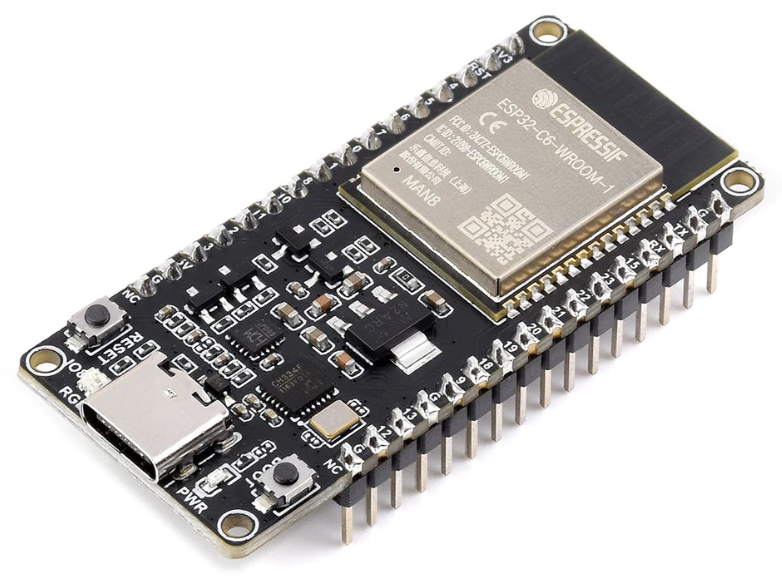
\includegraphics[width=0.3\textwidth]{Pictures/esp32.png}
  \caption{esp32}
  \label{fig:esp32}
\end{figure}
The ESP32 stands out as an exceptionally versatile and cost-effective
microcontroller. This particular microcontroller stands out due, to its 32 bit
architecture and the capability to run at a system clock speed of up to 240MHz
with the version utilised in this project operating at 160MHz. This ensures
processing power for handling demanding tasks.

A crucial aspect for a quadcopter is an attitude control system, which requires
a microcontroller of performing pulse width modulation (PWM) at high frequencies
preferably above 50Hz to ensure precise control over motor speeds. The ESP32s
PWM capabilities along with its 160MHz clock speed make it a great choice for
real time control operations. The strong community support and extensive
documentation further enhance its suitability for projects offering developers
an array of resources to utilise.

In the quadcopter project the ESP32 functions as the bridge between the
Raspberry Pi and the quadcopters hardware such, as speed controllers (ESCs) and
motors. It implements an attitude control algorithm written in python to
maintain stability and respond to navigation commands. Using UART communication
the ESP32 gets flight details from the Raspberry Pi, such, as orientations and
throttle configurations. It then sends back flight information to ensure
coordination of control systems for top notch flight efficiency. This
interaction showcases the ESP32s ability to operate within a system of
components proving its worth, in creating cutting edge aerial vehicles.

\section{Inertial Measurement Unit (IMU)}\label{IMU}
\begin{figure}[H]
  \centering
  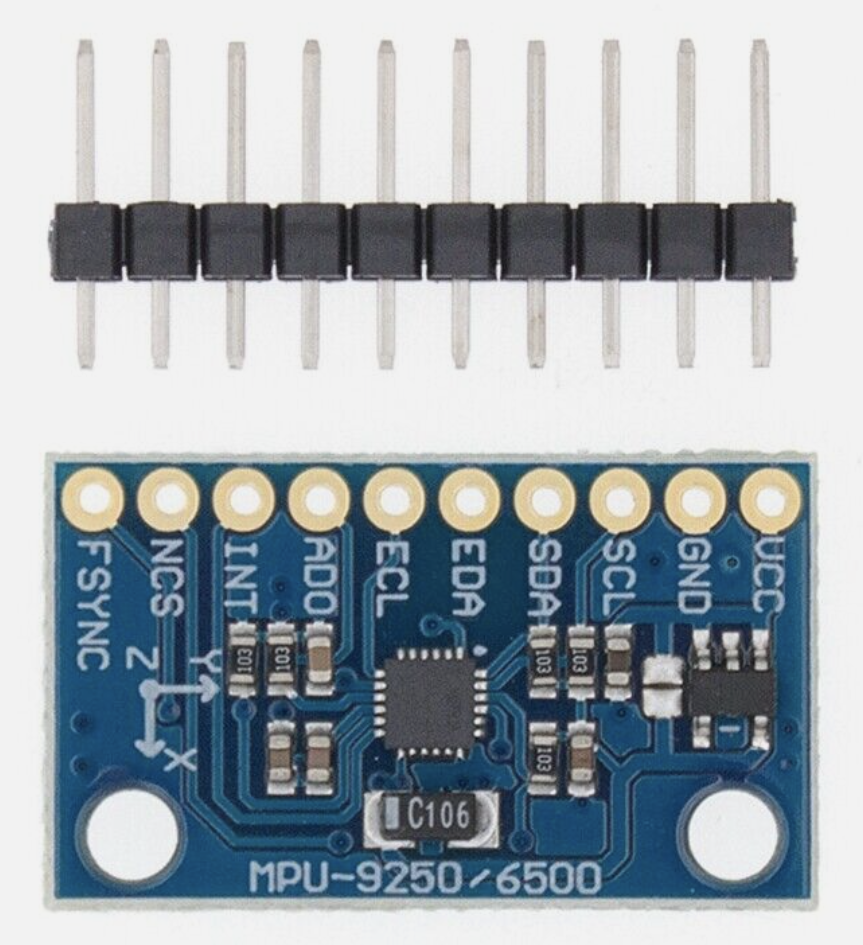
\includegraphics[width=0.2\textwidth]{Pictures/IMU.png}
  \caption{IMU}
  \label{fig:IMU}
\end{figure}
The MPU9250 integrates a 3-axis gyroscope, a 3-axis accelerometer, and a 3-axis
magnetometer. This 9 DoF capability allows it to provide comprehensive data on
the quadcopter's orientation, acceleration, and magnetic heading, enabling
precise control and stabilization.

Its small footprint makes it ideal for use in compact devices like quadcopters,
where space is at a premium and every gram of weight matters for flight
efficiency and duration.

The MPU9250 is designed for low power consumption, which is crucial for
battery-operated devices like quadcopters to maximize flight time.

It offers high-resolution sensor data, which is essential for maintaining stable
flight and accurate navigation in a quadcopter. This precision enables the
execution of complex manoeuvres and stability in various flying conditions. The
gyroscope in the MPU9250 offers selectable full-scale ranges of ±250, ±500,
±1000, and ±2000 degrees per second (dps). This allows for fine-tuning the
sensitivity based on the specific requirements of the quadcopter, enabling
precise measurement of rotational motion. The accelerometer provides selectable
full-scale ranges of ±2g, ±4g, ±8g, and ±16g. This adaptability allows the
device to accurately measure acceleration due to gravity and motion,
contributing to effective motion tracking and stabilization. The magnetometer
offers a full-scale range of ±4800 µT, allowing for precise measurements of the
Earth's magnetic field. This sensitivity is key for accurate heading
information, vital for navigation and maintaining a desired flight path.

The MPU9250's ability to output data from all nine sensors (gyroscope,
accelerometer, magnetometer) allows for advanced sensor fusion algorithms, such
as Kalman filtering, to provide highly accurate and reliable orientation and
motion data.

For the above reasons as well as its low cost the MPU9250 IMU has been chosen.

This project utilises both I2C and SPI protocols for communication, with the
MPU9250 IMU connected to the ESP 32 WROOM using the I2C protocol at a data
transmission rate of 400KHz. Through the I2C protocol, the ESP 32 WROOM, serving
as the master device on the bus, retrieves sensor data from the IMU, which
functions as the slave device. The MPU9250 IMU offers various configurable
measurement scales for its sensors, with the specific ranges employed in the
quadcopter being: Gyroscope ±2000 degrees per second (dps), accelerometer ±16g
and Magnetometer ±4800µT.

\section{ESC's (Electronic Speed Controller)}\label{esc}
\begin{figure}[H]
  \centering
  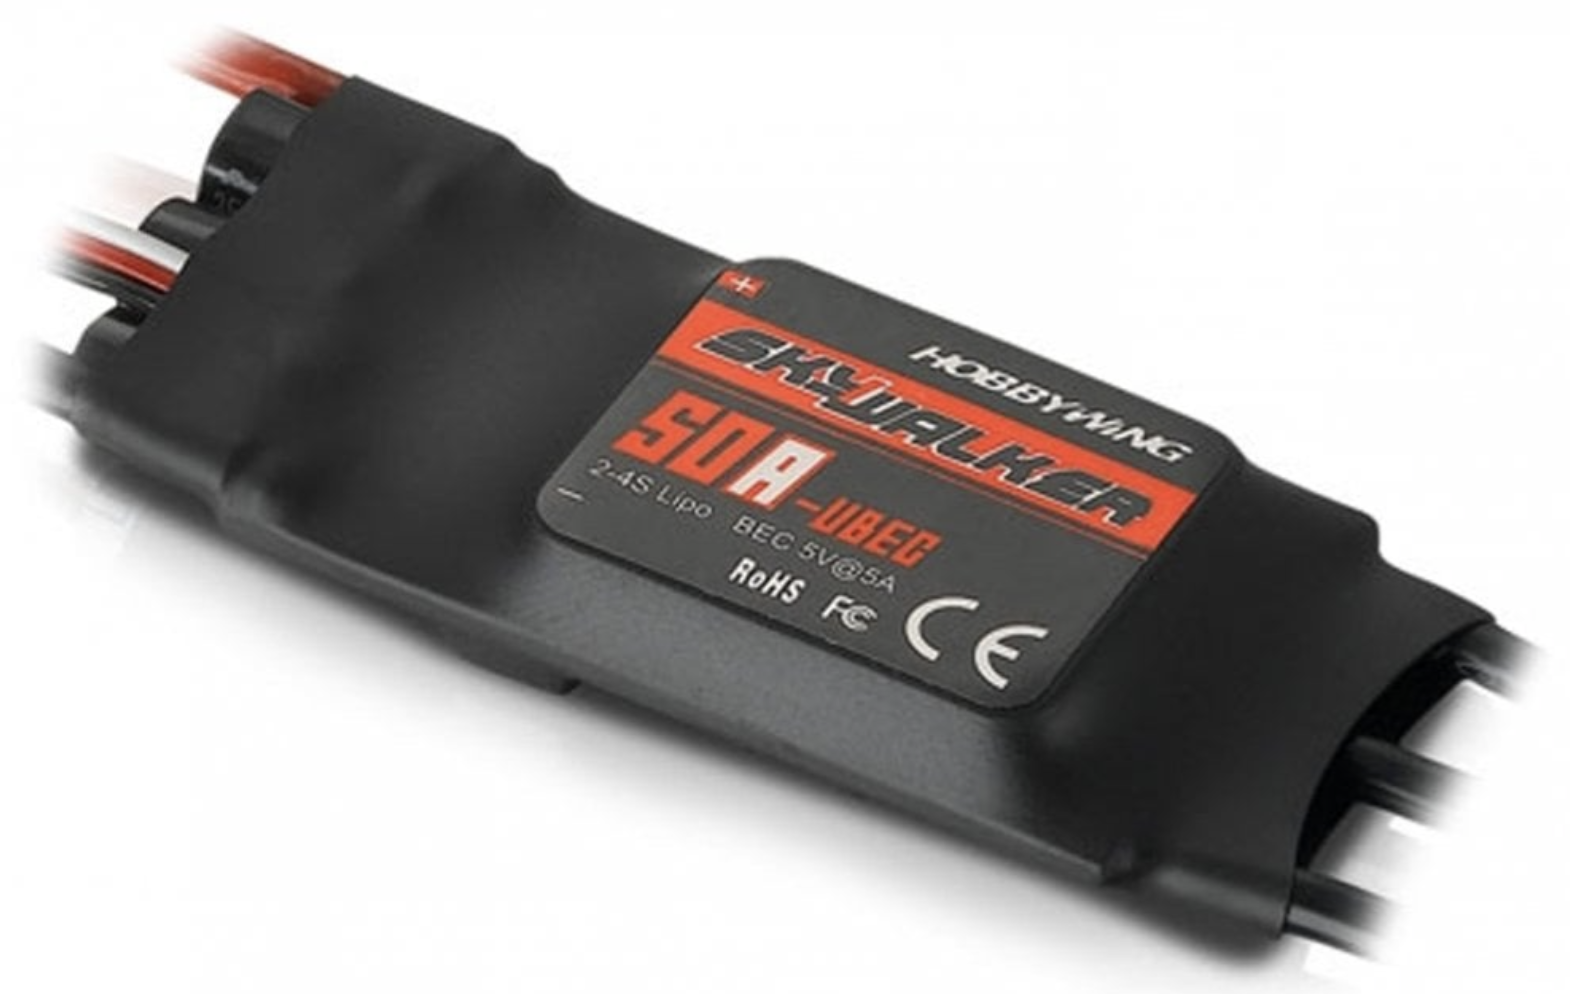
\includegraphics[width=0.35\textwidth]{Pictures/esc.png}
  \caption{ESC (Electronic Speed Controller)}
  \label{fig:esc}
\end{figure}
Designed specifically for quadcopters, the Skywalker 50A V2 is a brushless
electronic speed controller (ESC). It can withstand peaks of up to 70A and runs
at a constant 50A current, making it compatible with the motors above
(Section:\ref{motors}). This ESC has an integrated switch mode BEC with a 5A
output at 5V and is compatible with 4S LiPo batteries (Section:\ref{battery}).
To guarantee durability and dependability, it also offers a variety of
protection features such ESC heat protection and abnormal input voltage.

The ESC controllers work by receiving a digital signal, known as Pulse-Width
Modulation (PWM) which have a pulse, the 'width' of these pulses (i.e., how long
they stay 'on' versus 'off' in a given cycle) is adjusted to control the speed
of the motor. This is known as the duty cycle. A longer 'on' time (wider pulse)
means more power is delivered to the motor, making it spin faster. The ESC also
includes features like a built-in BEC to power flight controllers and safety
protocols for heat and voltage protection, ensuring reliable operation.

\section{Propellers}
\begin{figure}[H]
  \centering
  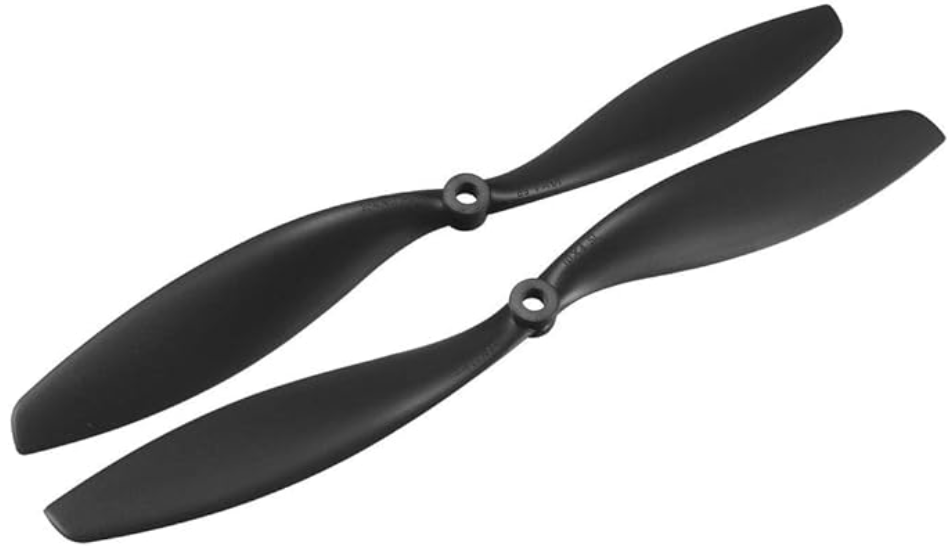
\includegraphics[width=0.35\textwidth]{Pictures/props.png}
  \caption{propellers}
  \label{fig:propellers}
\end{figure}
An essential part that greatly enhances the aircraft's performance and
manoeuvrability are the 1045 propellers. This specific quadcopter build is a
good fit for these propellers because of their 10 inch diameter and 4.5 inch
pitch, which combine to produce a balanced combination of thrust and efficiency. 

With '10' denoting the propeller's diameter in inches and '4.5' denoting its
pitch in inches, the identifier '1045' describes the propeller's measurements.
Understanding the pitch is essential to comprehending the propeller's thrust
capabilities and how it will work with the quadcopter's overall aerodynamic
design. Pitch is defined as the propeller's theoretical maximum airborne speed
in a single rotation, assuming perfect circumstances.

These propellers have a nice balance between strength and weight because they
are made of sturdy materials. This guarantees that the propellers can endure the
rigours of flight without significantly increasing the quadcopter's total mass,
which is crucial for preserving the best possible flight dynamics and
battery efficiency 

There are two variants for the 1045 propellers: clockwise (CW) and anticlockwise
(CCW). This is crucial for quadcopters because, in order to offset the
rotational torque generated by each motor and maintain stability and control
during flight, each propeller's rotation direction must alternate.

For more information on how these propellers generate thrust, counteract
rotational torque and allow for pitch roll and yaw manoeuvres please see
Section:\ref{Quadcopter_position_manipulation}
\section{Voltage Regulator}
\begin{figure}[H]
  \centering
  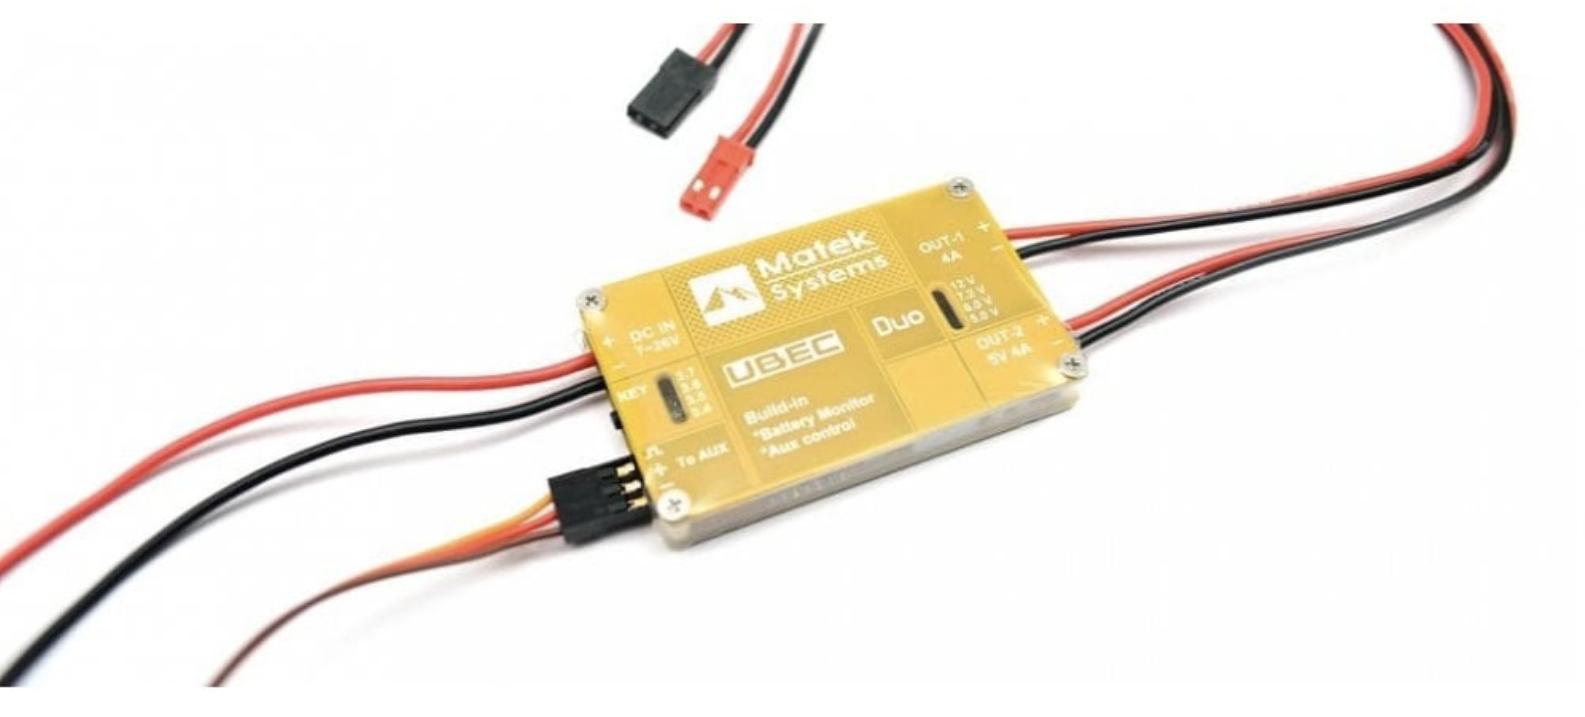
\includegraphics[width=0.35\textwidth]{Pictures/voltage_regulator.png}
  \caption{Voltage regulator}
  \label{fig:voltage_regulator}
\end{figure}

The  Matek Systems Matek - UBEC DUO is a dual-output voltage regulator that
offers flexible power management. Wide input voltage range support is provided,
and two output channels with substantial power management. While one channel can
be adjusted between 5V and 12V to accommodate different components, the other is
set at 5V and ideal for receivers or flight controllers.

The GNSS base station module and the flight controller/Raspberry Pi are powered
by the voltage regulator on the quadcopter. The GNSS base station is powered by
five volts, whereas the flight controller is powered by six, both modules are
powered from battery's seen in Figure:\ref{battery}.

\section{Battery}\label{battery}
\begin{figure}[H]
  \centering
  
\includegraphics[width=0.35\textwidth]{Pictures/battery.png}
  \caption{battery}
  \label{fig:battery}
\end{figure}
The GNB 5500mAh 4S 70C LiPo Battery with an XT90 connector is a The GNB 5500mAh
4S 70C LiPo Battery with an XT90 connector is a high-capacity, high-discharge
battery designed for use in various remote-controlled (RC) applications. This
5500mAh battery is perfect for long flight times because it keeps a substantial
charge and allows for longer use between recharges.

With four cells connected in series, this battery has a 4S1P configuration,
producing a nominal voltage of 14.8V. Our high-performance quadcopter needs a
lot of power to run due to its weight. This 70C continuous discharge rate
shows the battery maintains a steady power flow even while it is under the heavy
load of the quadcopter. The battery can safely discharge in this scenario at a
rate of 70 times its capacity, or 385A, which provides sufficient power for
demanding applications.

The battery also has a burst discharge rate of 140C, which enables brief bursts
of even higher power output up to 770A. This feature is helpful in situations
where immediate action or rapid acceleration is required. Maintaining
performance and safety requires a dependable connection that can handle high
current without producing a lot of heat, which is what the XT90 connector
offers.

The battery's weight and dimensions are indicative of its high capacity and
voltage. Its dependability and longevity are further increased by the inclusion
of safety features like short-circuit protection, overcharge and overdischarge
prevention, and others. Like this one, the majority of LiPo batteries also
include a balancing plug, which is often a JST-XH connector and is used for
balance charging. This keeps the battery's general health and efficiency intact
by ensuring that each cell is charged equally.

\section{Sensors}
This section outlines the various different sensors that were used on the
quadcopter, delving into the specs, compatibility and test performance. The
analysis includes an examination of the sensors' roles in navigation,
stabilization, and telemetry data acquisition.

\subsection*{GNSS modules}
\subsection{GNSS Rover Module}
  \begin{figure}[H]
    \begin{minipage}{0.5\textwidth}
      \centering
      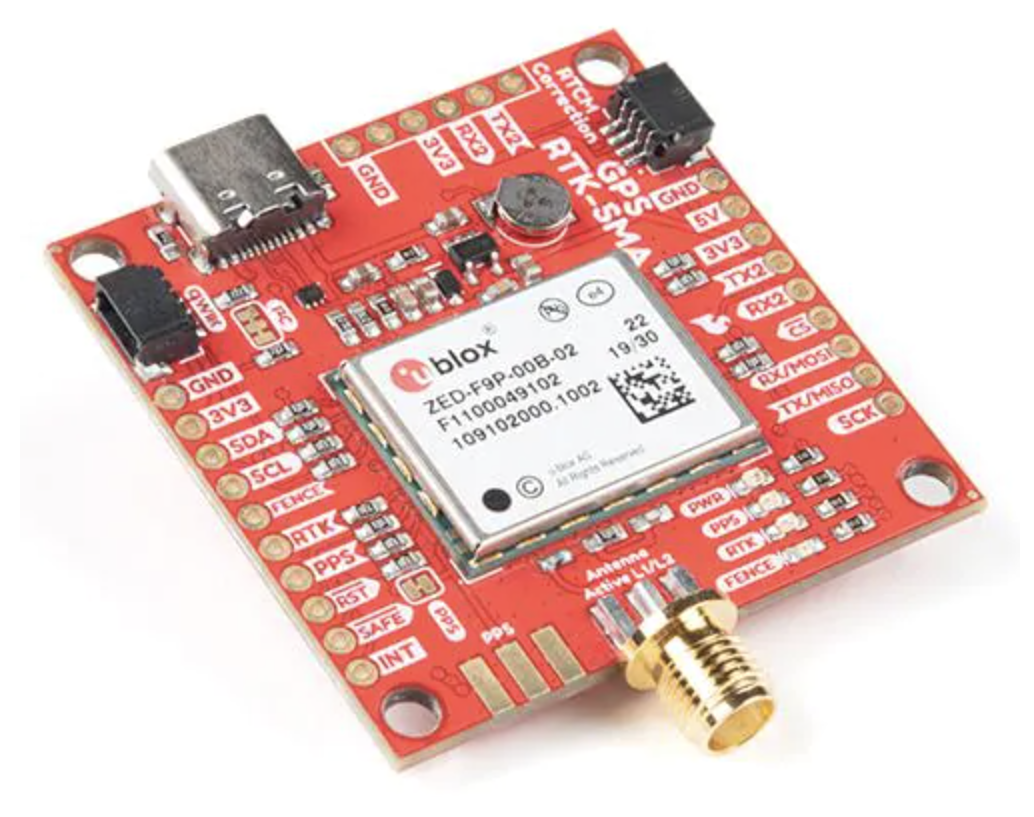
\includegraphics[width=0.5\textwidth]{Pictures/gnss_rover.png}
      \caption{GNSS Rover module}
      \label{fig:gnss_rover}
    \end{minipage}
    \begin{minipage}{0.5\textwidth}
      \centering
      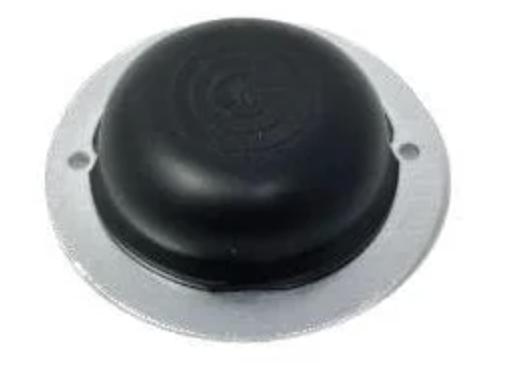
\includegraphics[width=0.5\textwidth]{Pictures/quad_antenna.png}
      \caption{Quadcopter antenna}
      \label{fig:Quadcopter antenna}
  \end{minipage}
\end{figure}
The SparkFun GPS-RTK-SMA Breakout - ZED-F9P Fig.\ref{fig:gnss_rover} will prove
to be a good option for my onboard GPS module due to its precise GNSS
capabilities. It is significantly better than the MikroElektronika GPS Click
featuring the LEA-6S, especially in its technical specification. The u-blox
ZED-F9P module within, is known for high accuracy and multi- band GNSS support
with a maximum update frequeccy of 25Hz. This allows the quadcopter to utilise
real-time kinematic (RTK) positioning which is great for applications which need
centimetre level signalling \cite{sbg_systems_2024}. Ensures comprehensive
coverage and reliability due to its ability to access a wide range of satellite
systems (GPS, GLONASS, Galileo, and BeiDou). This should prove ideal for getting
centimeter accurate data for the quadcopter, hence gaining precise position
control on the quadcopter.

To complement the capabilities of the GNSS rover module, it is coupled with the
Tallysman 33-SSL889XF L1/L2 GNSS Antenna. This pairing is key to maximizing the
performance of the ZED-F9P module, as the Tallysman antenna is designed to
optimize signal reception and accuracy for L1/L2 frequencies. Such an
integration ensures that the quadcopter benefits from the best possible GNSS
performance, crucial for maintaining high precision and reliability in
navigation and positioning tasks. This setup is expected to provide the
quadcopter with unparalleled precision in its operations, making it
exceptionally suited for tasks in accuracy in position control.

For testing evaluation on this module please see Section:\ref{GNSS_rover_module}

\subsection{GNSS Base Station}\label{GNSS_base_station}
\begin{figure}[H]
  \begin{minipage}{0.5\textwidth}
    \centering
    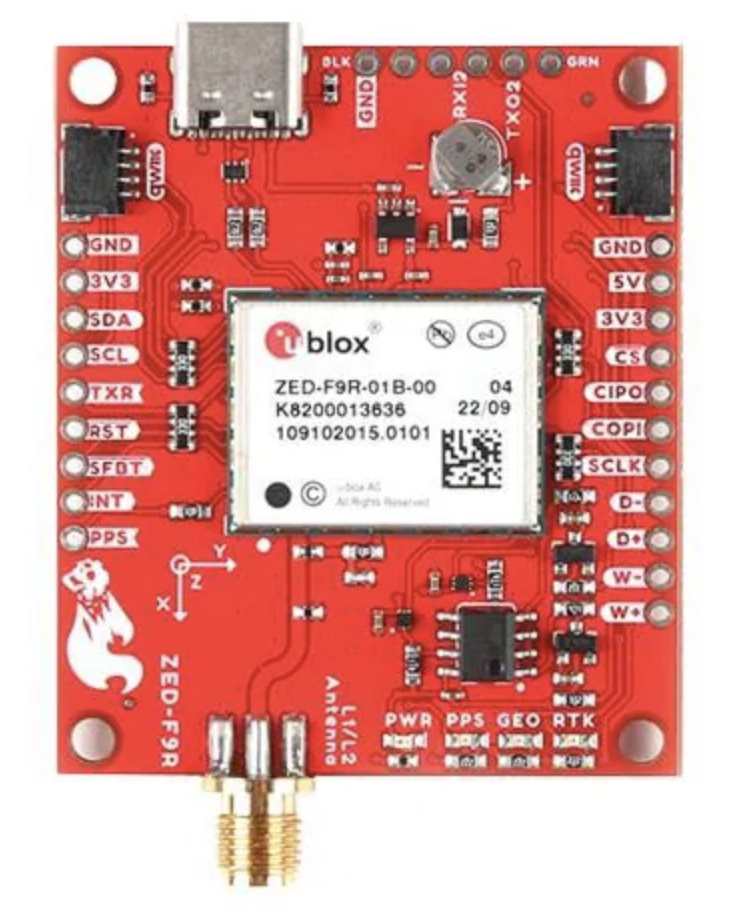
\includegraphics[width=0.5\textwidth]{Pictures/gnss_base_station.png}
    \caption{GNSS Base Station module}
    \label{fig:gnss_base_station}
  \end{minipage}
  \begin{minipage}{0.5\textwidth}
    \centering
    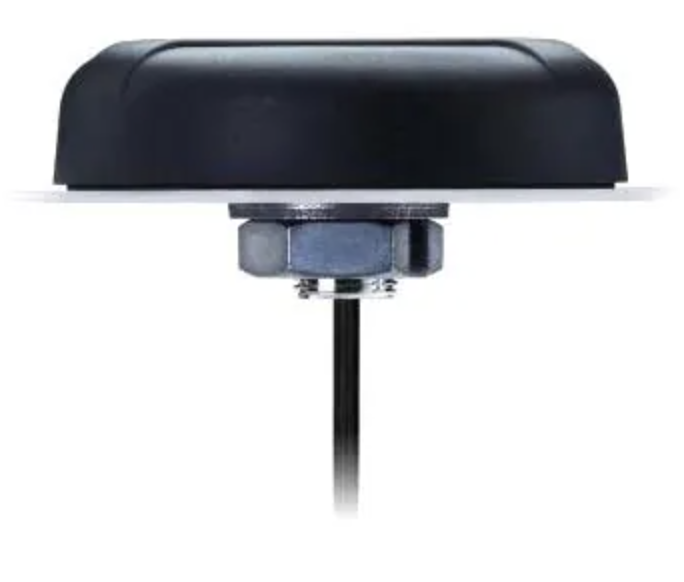
\includegraphics[width=0.5\textwidth]{Pictures/base_station_antenna.png}
    \caption{Base Station antenna}
    \label{fig:base_station_antenna}
  \end{minipage}
\end{figure}
The SparkFun GPS-RTK Dead Reckoning Breakout - ZED-F9R
(Fig.\ref{fig:gnss_base_station}) features make it a highly sophisticated option
for GPS-related applications. The modules feature a 184-channel u-blox F9 engine
GNSS receiver which will receive signals from GPS, GLONASS, Galileo, and BeiDou
constellations with 0.2-meter accuracy with a maximum update frequeccy of 25Hz.
This makes it a superior choice when utilising base station NTRIP technology as
well as RTCM (Radio Technical Commission for Maritime Services) messages to
communicate correction data to the onboard GNSS module.

The Taoglas A.80 L1/L2 GNSS Antenna is used in conjunction with the GNSS module
to support its exceptional performance. This antenna is a perfect fit for the
ZED-F9R module because it is specifically made to improve signal reception and
accuracy for L1/L2 frequencies. Advanced navigation and autonomous
flying systems depend on high positioning precision and dependability, which is
ensured by the synergy between the Taoglas antenna and the GNSS module when
provinding the GNSS rover module above with RTCM correction data. Even in
challenging conditions, this combination offers a reliable way to provide exact
position tracking and navigation capabilities.

For testing evaluation on this module please see Section:\ref{GNSS_rover_module}

\subsection{Base station container and stand}
\begin{figure}[H]
  \begin{minipage}{.5\textwidth}
    \centering
    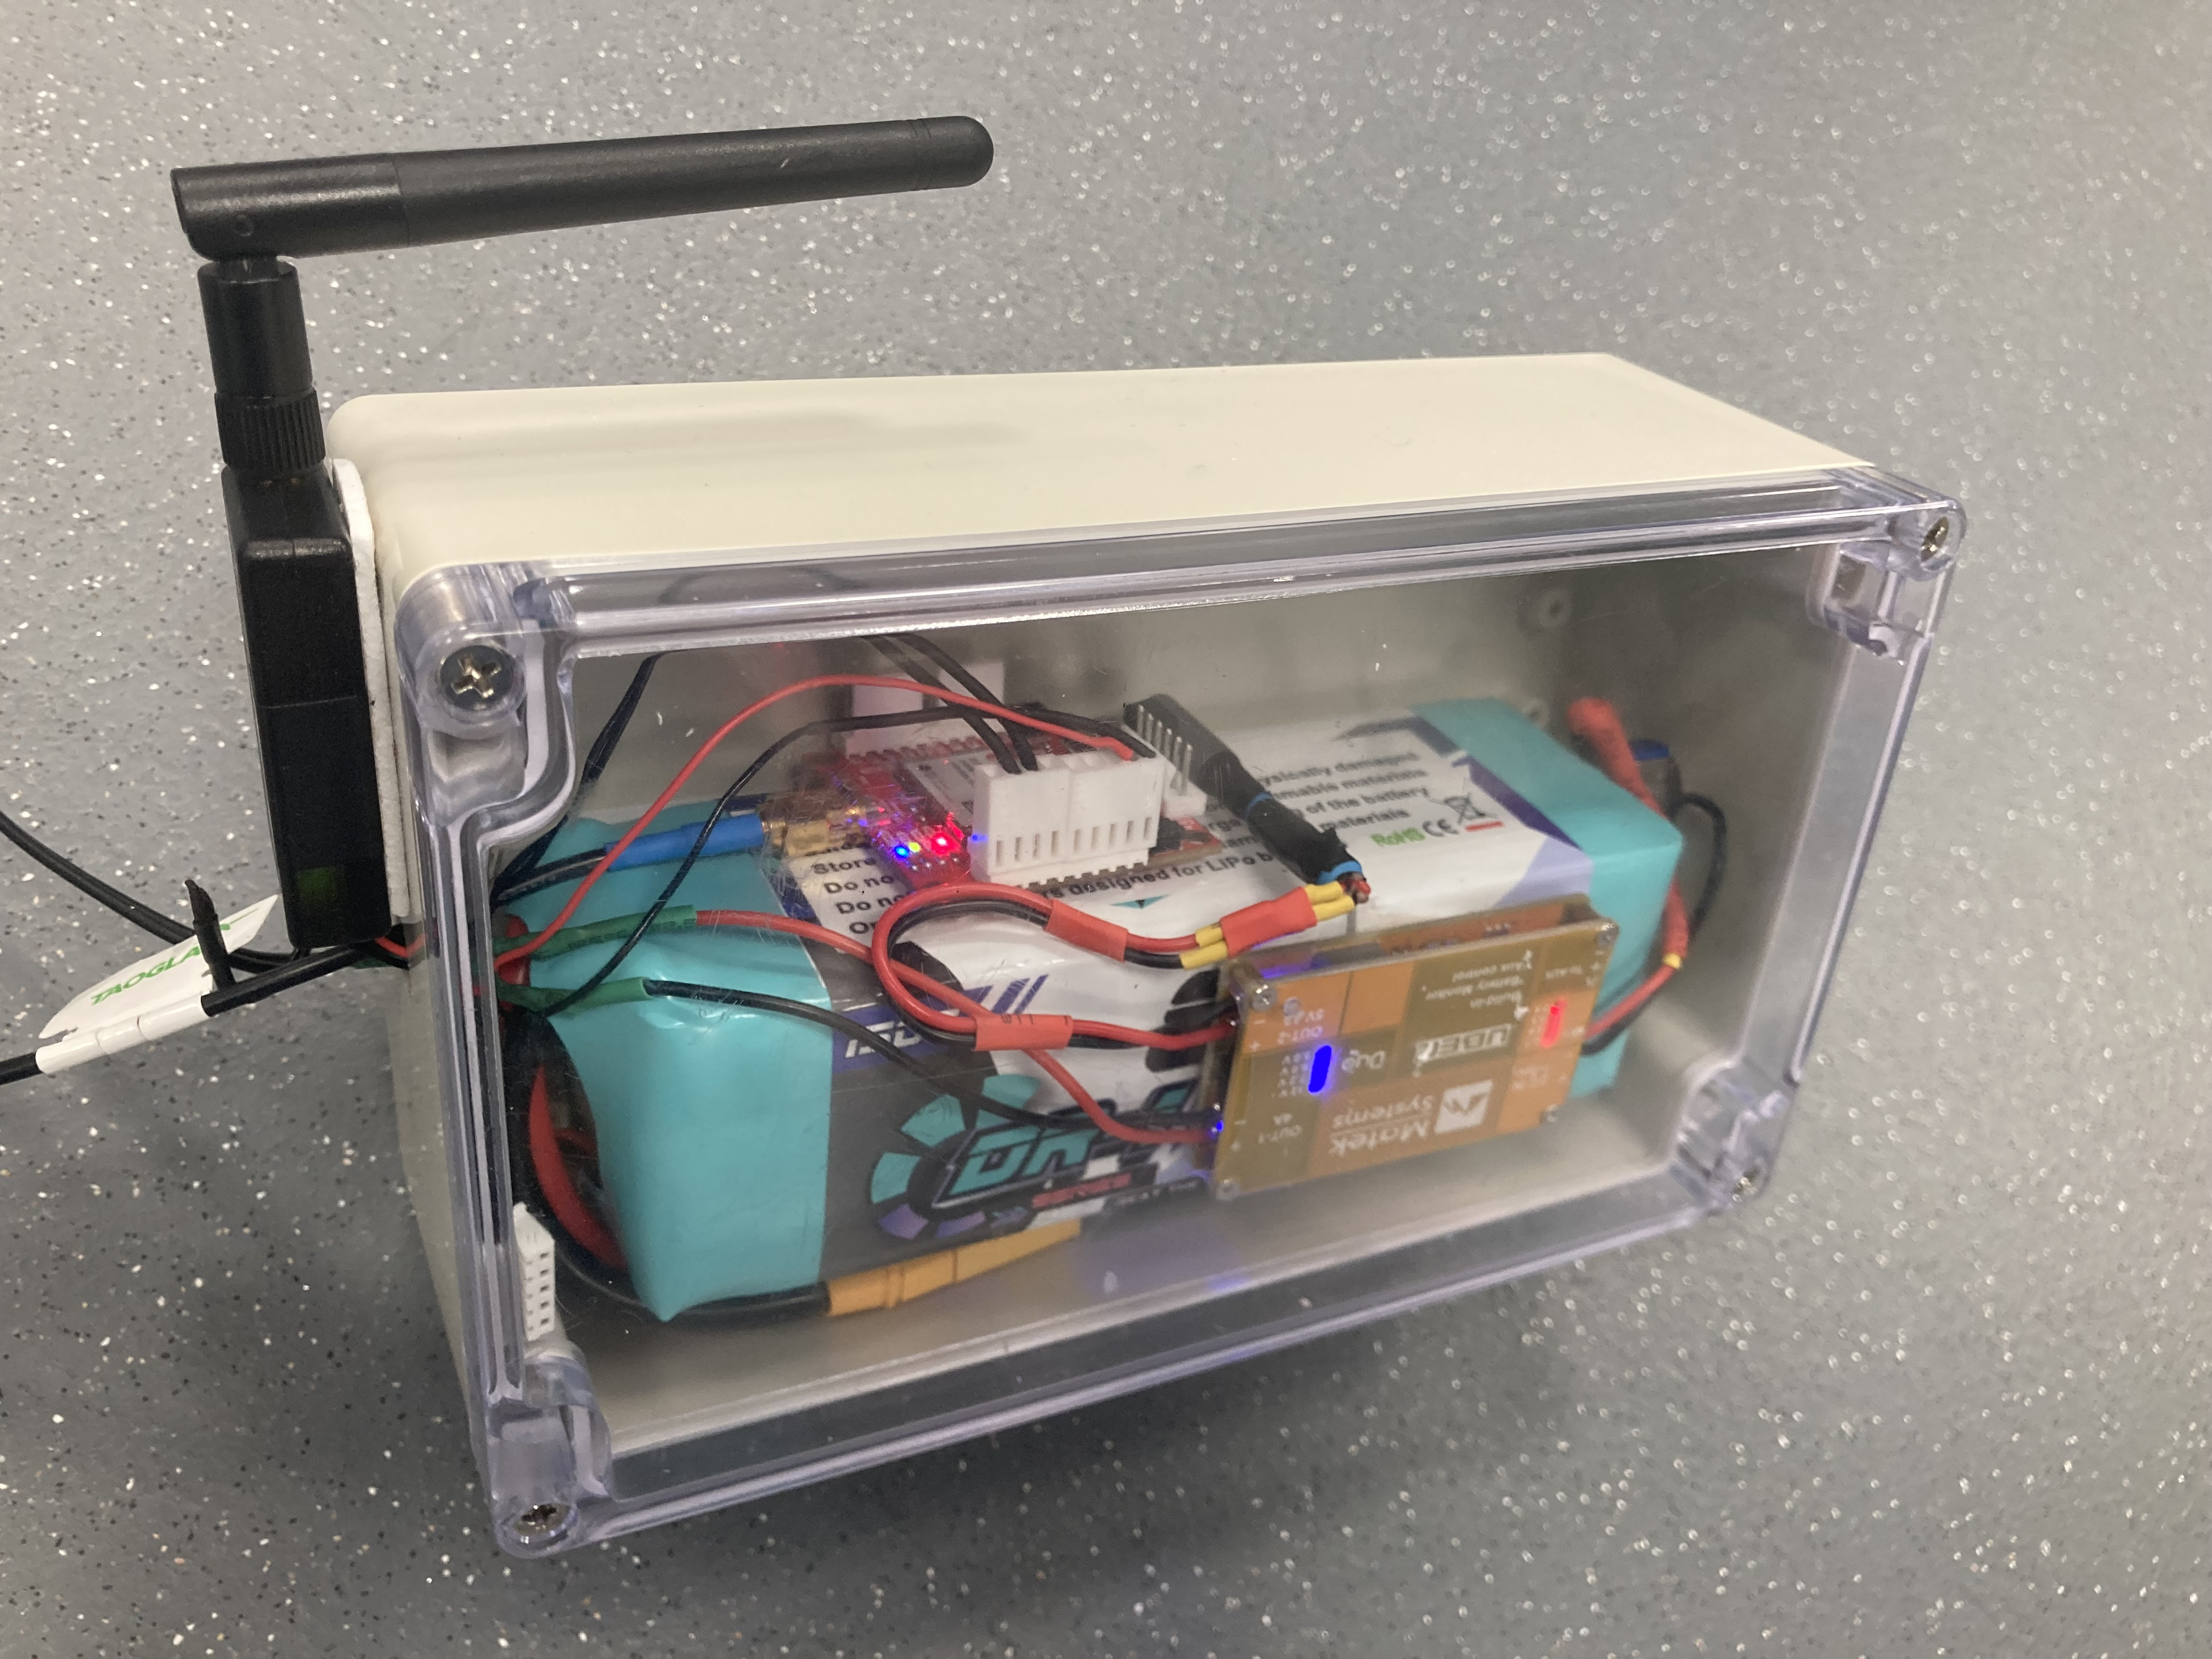
\includegraphics[width=0.7\textwidth]{Pictures/base_station_box.png}
    \caption{Base station container}
    \label{fig:Base_station_container}
  \end{minipage}
  \begin{minipage}{.5\textwidth}
    \centering
    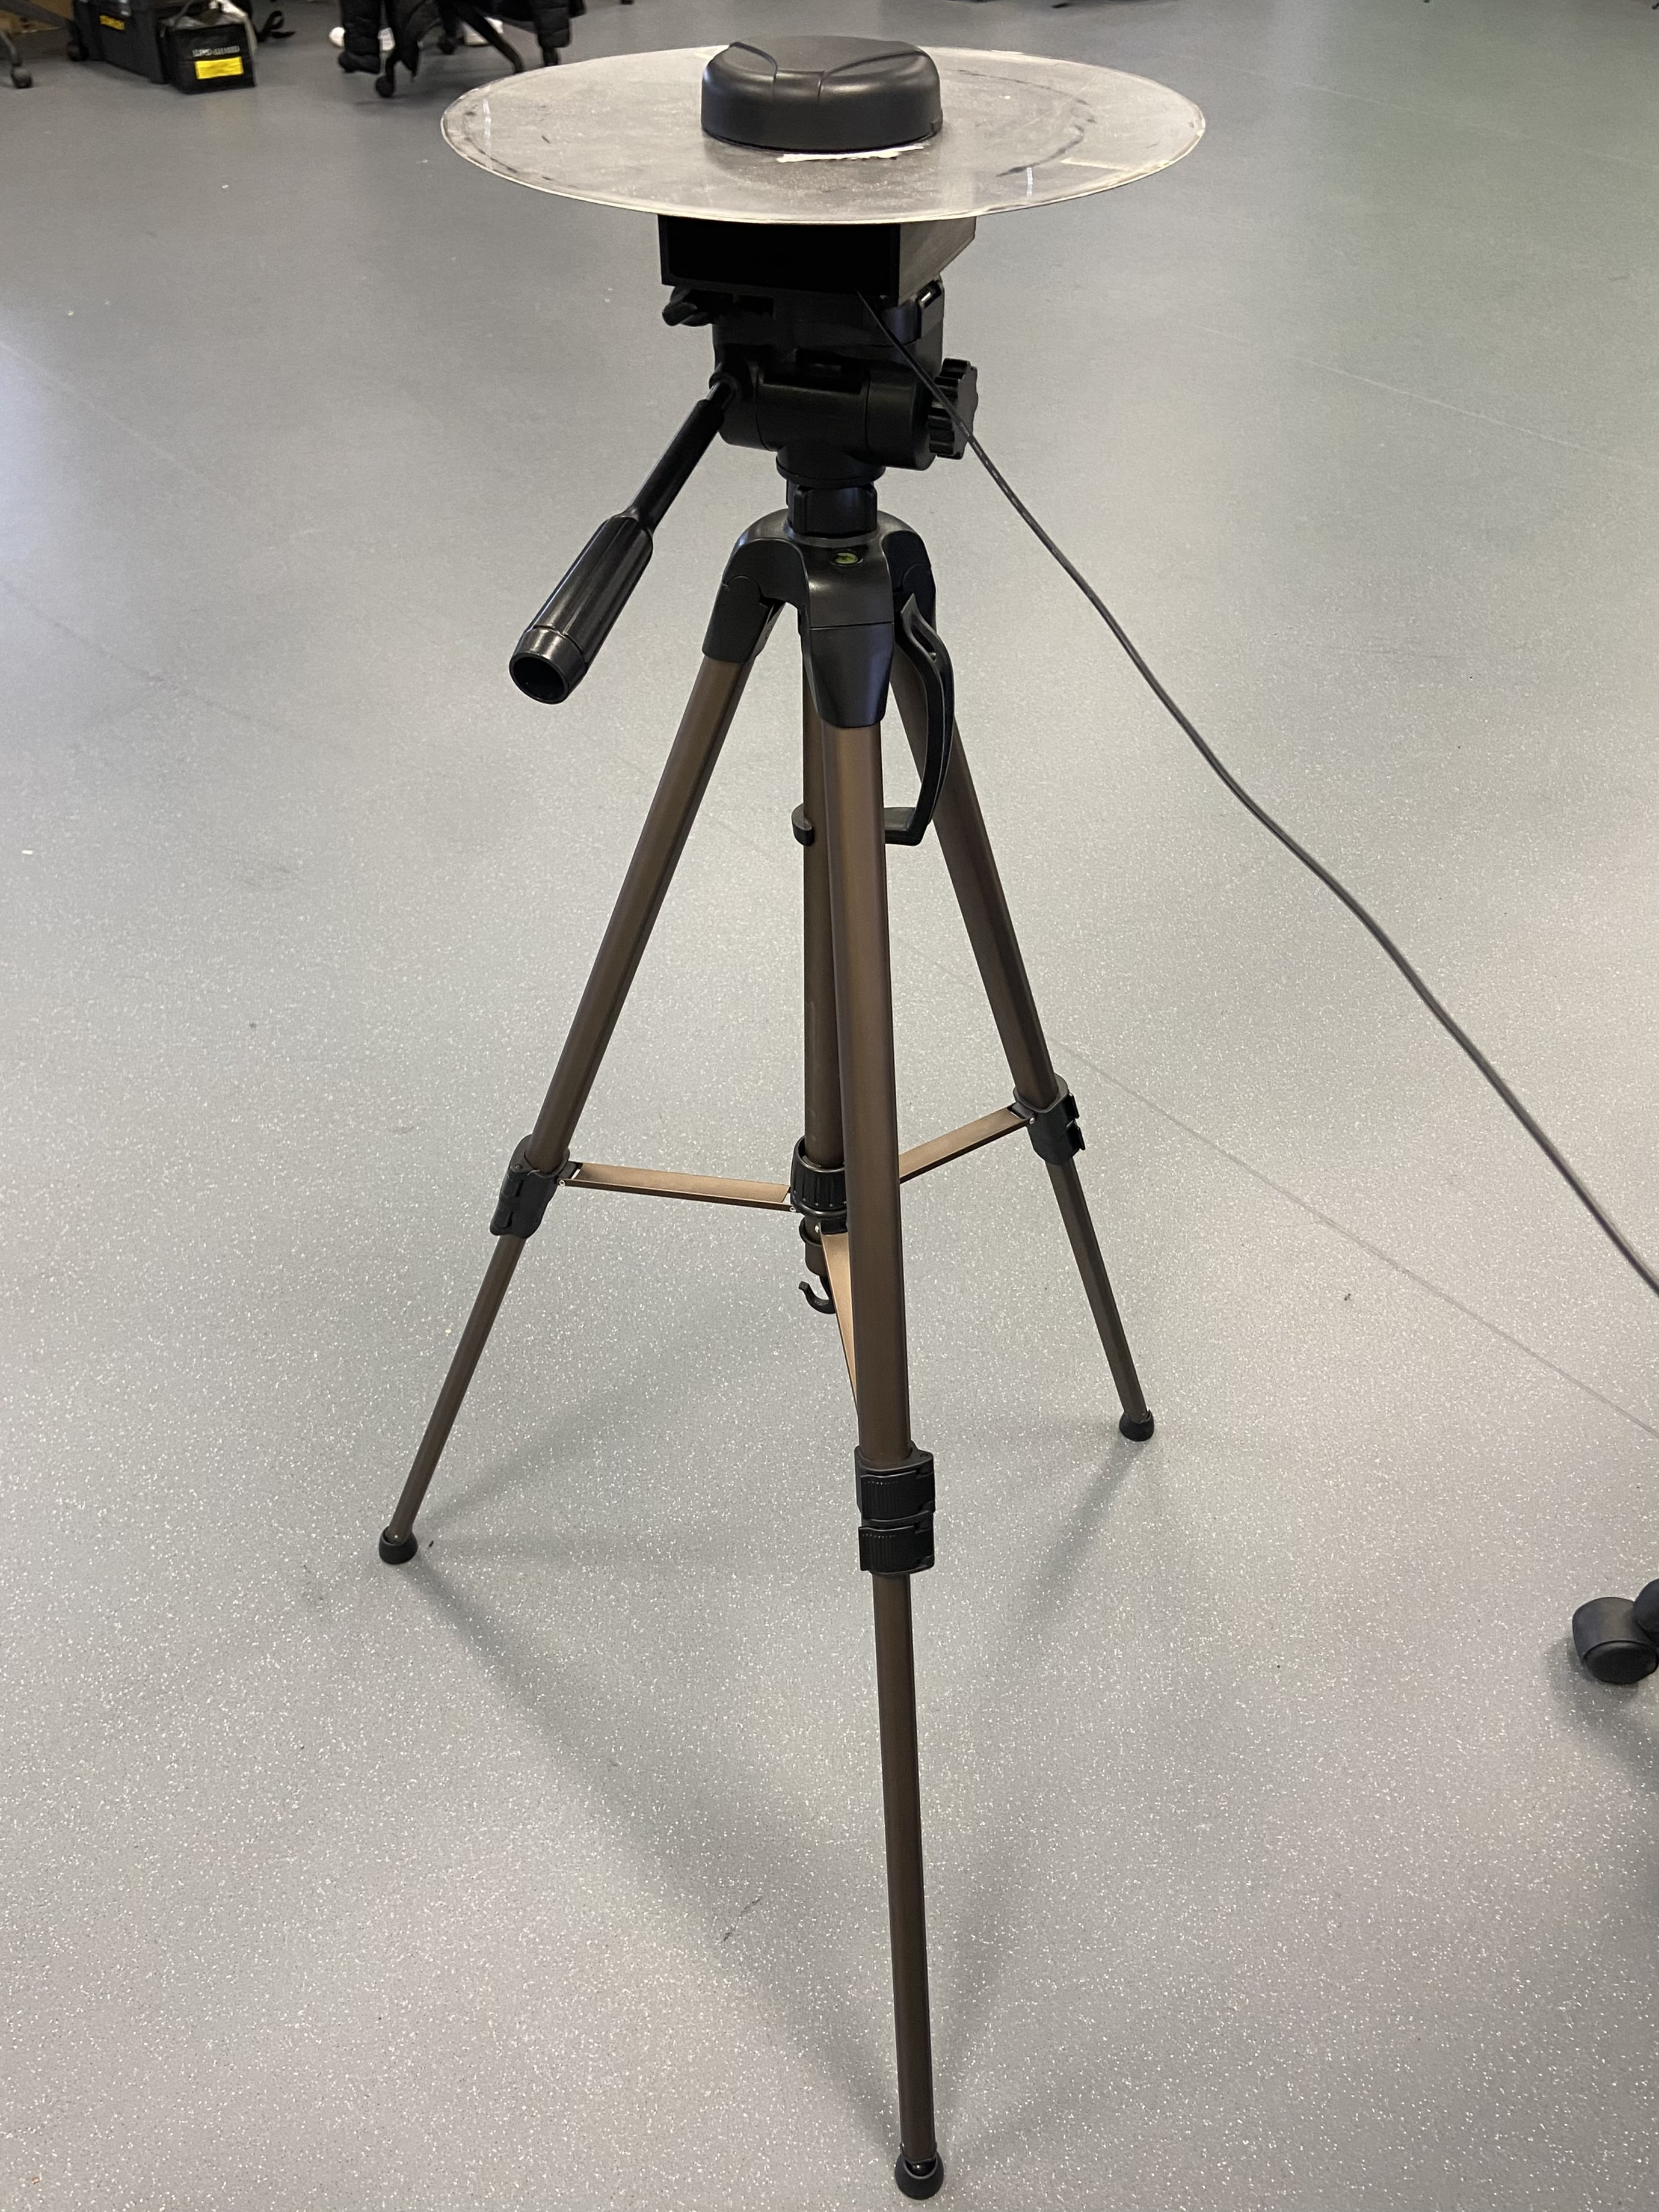
\includegraphics[width=0.4\textwidth]{Pictures/base_station_stand.jpg}
    \caption{Base station stand with antenna}
    \label{fig:Base_station_stand}
  \end{minipage}
\end{figure}
A container was designed (Figure:\ref{fig:Base_station_container}) to guarantee
the base station's component organisation and water resistance. The GNSS base
station module (Figure:\ref{fig:gnss_base_station}), a battery
(Figure:\ref{fig:battery}), and a voltage regulator
(Figure:\ref{fig:voltage_regulator}) were all kept secure from water damage
within this container. To ensure clear contact with the GNSS rover module, the
telemetry radio—which is essential for transmitting correction data—was placed
strategically on the outside (Figure:\ref{fig:gnss_rover}).

An essential part of the high-performance GNSS base station module is
the Taoglas A.80 L1/L2 GNSS Antenna (Figure:\ref{fig:base_station_antenna}). In
order to ensure that the base station can efficiently support precise
positioning for the GNSS rover module, this antenna was installed on a tripod to
secure its position and optimise signal reception
(Figure:\ref{fig:Base_station_stand}) for RCTCM corrections. 

\begin{figure}[H]
  \centering
  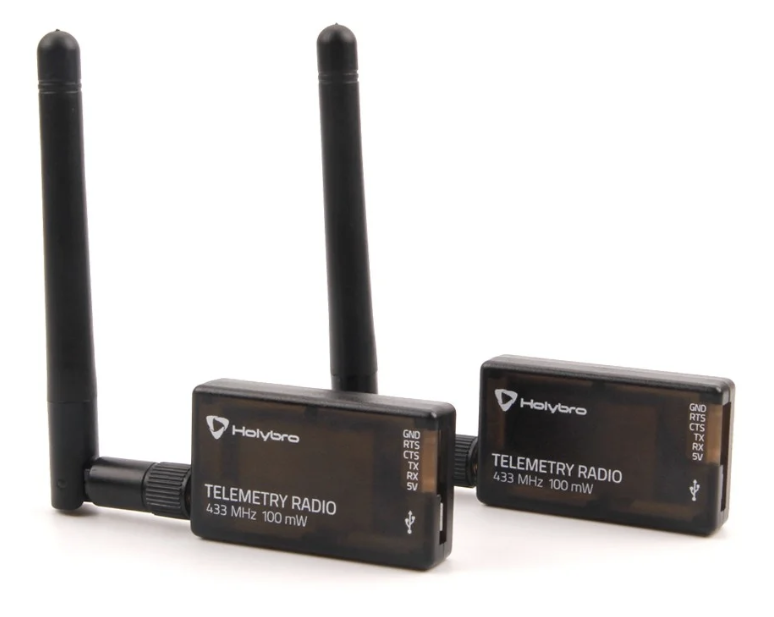
\includegraphics[width=0.3\textwidth]{Pictures/telemetry radio.png}
  \caption{telemetry radio for transmitting correction data}
  \label{fig:telemetry_radio}
\end{figure}
The Holybro SiK Telemetry Radio V3 100mW 433MH 915MHz
(Fig\ref{fig:telemetry_radio}) will be used to transmit the RCTCM data from the
base station to the on board GNSS module to provide it with the necessary
correction data mentioned above. This radio is a lightweight and typically
offers a range of over 300 meters. It's important to ensure that the radio
telemetry is properly configured to communicate with the GNSS module. This
involves setting up parameters such as frequency, power output, and the
transmitting of RCTCM data.

\subsection{GNSS Calibration (U-center)}
The U-center software, created by u blox is a tool used for setting up, testing
and assessing GNSS module data. It offers a range of features to adjust
communication ports, protocols, data rates and message settings that are
essential, for enhancing the performance of GNSS receivers. Additionally
U-center plays a role in updating firmware to ensure GNSS modules operate with
the relevant enhancements.

In terms of visuals U-center provides real time data display showing satellite
tracking details, signal strengths and other important GNSS information. It
presents coordinates, altitude measurements, velocity data and offers detailed
insights into the accuracy and reliability of the GNSS data including estimates
on positional accuracy. This detailed information is crucial for evaluating the
precision and functionality of GNSS modules across applications.

When configuring modules like the SparkFun GPS RTK SMA Breakout. ZED F9P to
output GNGGA for altitude and GNGLL for latitude and longitude settings, in
U-center involves connecting the module to the software interface. By accessing
the Configuration View within U-centers interface users can enable desired NMEA
messages while disabling others to streamline output. Saving these
configurations in the module's non volatile memory ensures they are maintained
through power cycles. When it comes to how updates are made, the SparkFun GPS
RTK SMA Breakout ZED F9P and SparkFun GPS RTK Dead Reckoning Breakout ZED F9R
can both handle update rates of, up to 25 Hz. This rapid update frequency is
ideal for tasks that demand fast results. The ZED F9R, equipped with built in
sensors brings advantages for dead reckoning by delivering improved accuracy and
consistency even in tough conditions.

To establish a base station that solely outputs RTK corrections you simply need
to set the GNSS modules mode to function as a base station choose the RTK
correction messages, in this case RTCM3 is used, and specify the output via the
correct communication port. These adjustments guarantee that the base station
transmits RTK corrections ensuring efficient and accurate data transmission. In
order to get the most reliable RTK data from the base station, the 'survey in'
feature was used. During the Survey-in process, the base station collects GNSS
data over time, and this data is used to calculate a more reliable and stable
coordinate estimate of its location. For our particlar use case we wanted the
base stations position to be as accurate as possible, in order to achieve this
the minimum duration for the survey and the desired positional accuracy were set
to 5 minutes and 0.2m, ensuring that the base station's location is determined
with high confidence before it begins to transmit the  RTK corrections to rover
unit.

By integrating these functionalities and setups we can attain high levels of
precision and dependability in our GNSS modules, highlighting U-center as a
vital tool in satellite navigation practices.

\subsection{Time of Flight sensor}
\begin{figure}[H]
  \centering
  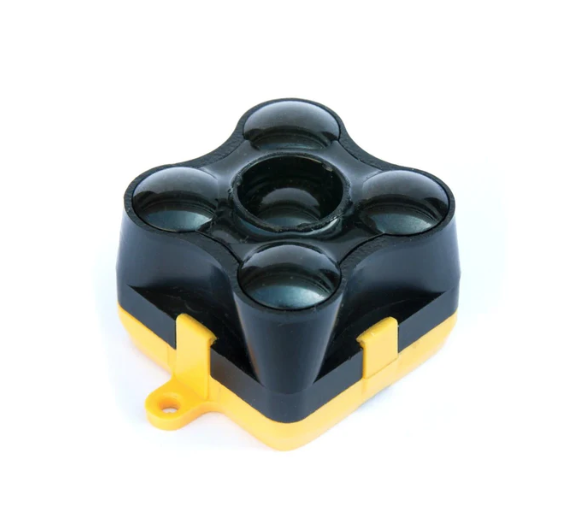
\includegraphics[width=0.3\textwidth]{Pictures/ToF_sensor.png}
  \caption{Time of Flight sensor}
  \label{fig:ToF}
\end{figure}
The ToF sensor used to measure the altitude of the drone is shown in Figure
\ref{fig:ToF} is the TR-EVO-60M sensor utilises infrared Time-of-Flight
technology to detect objects at distances ranging from 0.5 to 60 meters indoors
and 0.5 to 10-60 meters outdoors. With an impressive update rate of up to 240
readings per second, it ensures real-time data collection. Accuracy varies from
±4cm within 14m to 1.5\% beyond 14m, and it provides a minimalistic Field of
View of approximately 2°. The device requires a 5V DC power supply, with an
operational current between 90mA to 330mA. Communication is versatile, with USB,
UART, and I2C options available, and it features a Micro USB connector. Its
compact dimensions are approximately 29x29x22mm, with a feather-light weight of
9g for the sensor and an additional 3g for the backboard, totalling 12g. The
device is also CE certified for eye safety.

\subsection{Barometer}
\begin{figure}[H]
  \centering
  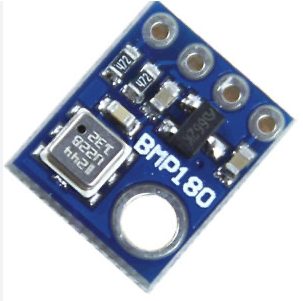
\includegraphics[width=0.2\textwidth]{Pictures/bmp180.png}
  \caption{Pressure sensor}
  \label{fig:bmp180}
\end{figure}
The BMP180 Digital Barometric Pressure Sensor Module seen in Figure
\ref{fig:bmp180} is perfect for applications including weather and altitude
monitoring dues to its compactness, low-power demand and cost effectiveness. It
ensures efficiency in battery-powered devices with as little as 0.5 microamperes
at 1Hz. With a precision of up to 0.02 hPa—which translates to an altitude
detection difference of 17 cm—the sensor offers exceptionally low noise levels.
Its pressure measuring range is 300 hPa to 1100 hPa, which allows it to track
altitudes from +9000 metres above sea level to about -500 metres below sea
level. The module can work between 1.8 and 3.6 volts in the supply voltage range
and can communicate at up to 3.5 MHz using an I2C interface.

\subsection{Anemometer}
\begin{figure}[H]
  \centering
  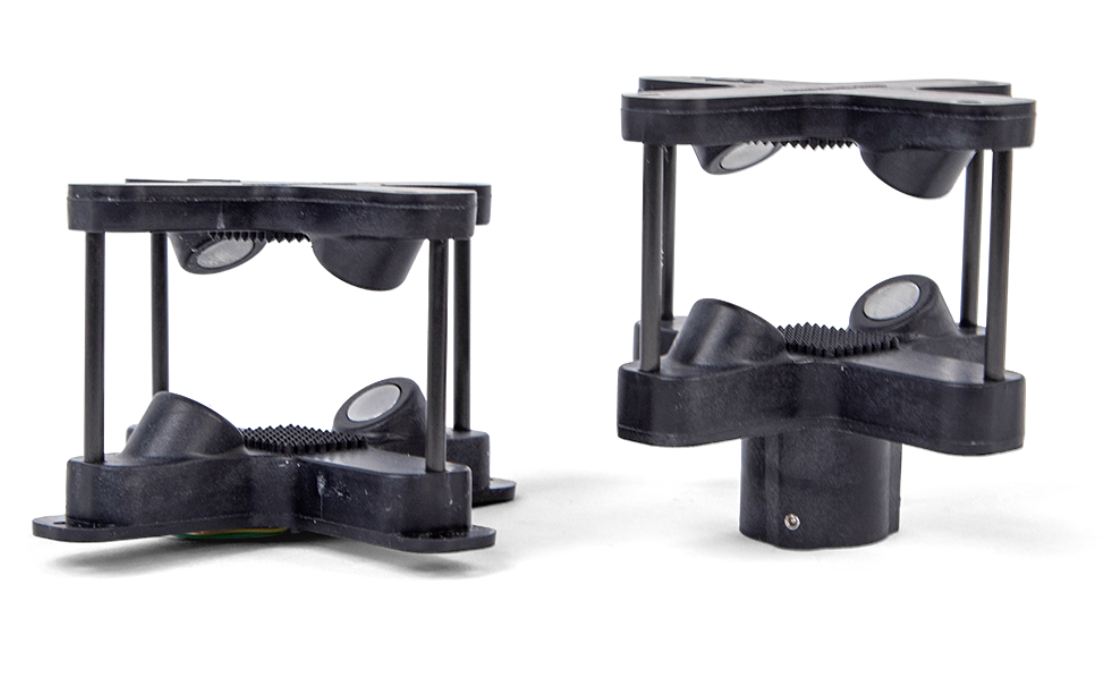
\includegraphics[width=0.4\textwidth]{Pictures/Anemometer.png}
  \caption{Anemometer}
  \label{fig:Anemometer}
\end{figure}

For the purpose of detecting wind speed, the quadcopter's sensor package
includes an anemometer, The LI-550 TriSonica Mini in
Figure:\ref{fig:Anemometer}. Real-time wind measurements are essential for the
aircraft's stability and manoeuvrability, particularly when performing precise
duties like surveying or search and rescue missions \cite{uav_wilderness_sar}.
This advanced anemometer, capable of operating within a broad voltage range of 5
- 32 V and consuming a modest power of 400 mW,ensures reliable performance even
in the most demanding environments. With its robust design, the anemometer
remains functional at altitudes up to 5000 meters and within a wide temperature
range of -20 to 72 °C, making it versatile for various atmospheric conditions.

High-tech instruments called ultrasonic anemometers like the LI-550 TriSonica
Mini, are used to measure wind directions and speeds very precisely. The system
uses the differential time of flight of ultrasonic pulses between pairs of
sensors placed at key angles to function. The device determines wind velocity
and bearing by computing the variance when wind modifies the speed of these
pulses, with an accuacy of 0.2m/s.

The device's high-resolution wind direction readings, which span a range of 0 to
359°, further highlight its remarkable precision in wind speed and direction
measurements and guarantee accurate navigation corrections. Real-time,
high-fidelity wind data can be obtained using the anemometer's advanced design,
which permits a maximum sampling frequency of 40 Hz and ultrasonic frequency
settings around 60 kHz. The anemometer's lightweight design, weighing only 50–67
grammes, ensures that its sophisticated features won't negatively affect the
quadcopter's payload.

The sensitivity, resolution, and reaction time of the sensor are critical in
delivering real-time analytics for the quadcopter's navigation system and data
gathering goals. Therefore, in order to accomplish a thorough analysis and
improve the quadcopter's capacity to adjust to abrupt gusts or changing wind
patterns, this sensor can provide high-resolution data in three-dimensional
space.
\section{Hardware schematic}
\begin{figure}[H]
  \centering
  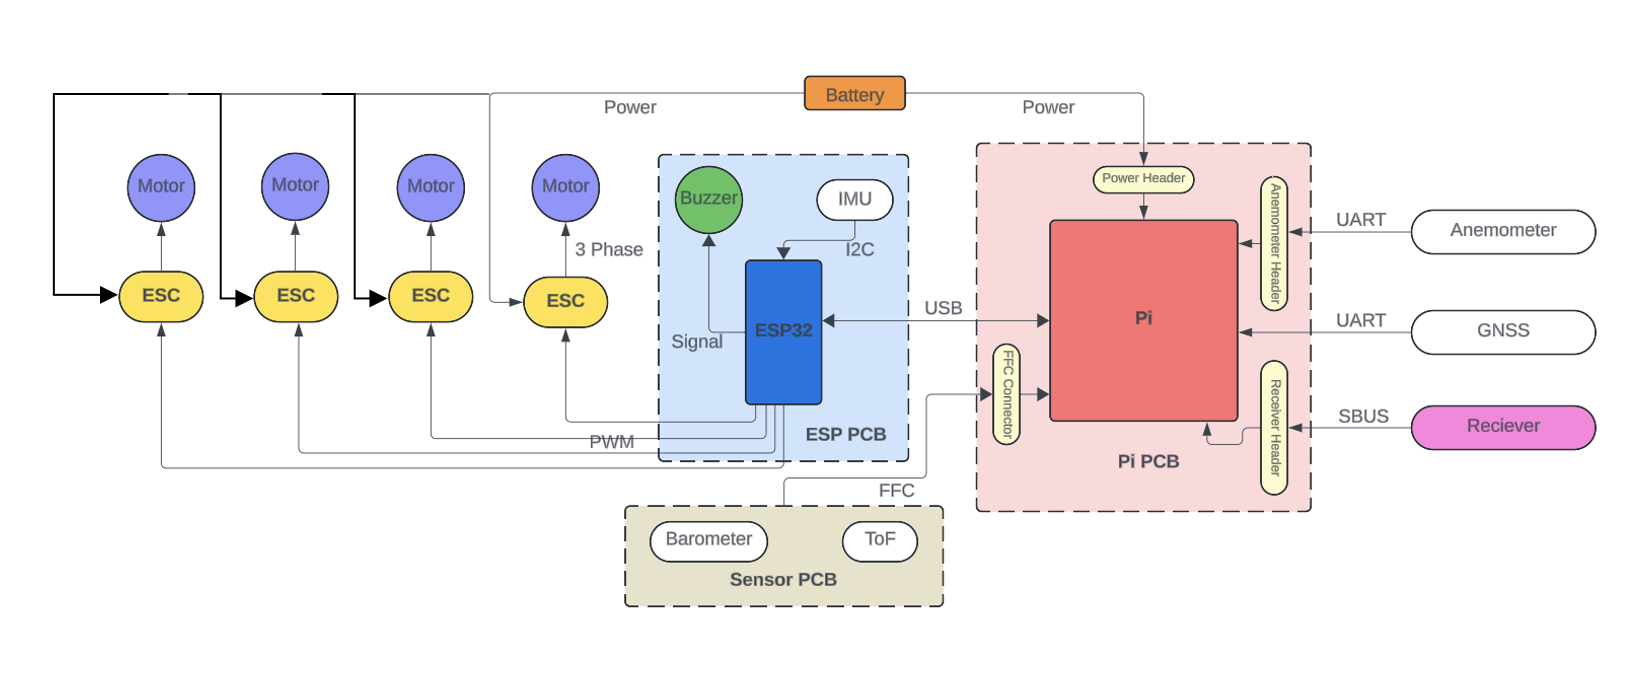
\includegraphics[width=1\textwidth]{Pictures/Hardware_schematic.png}
  \caption{Hardware schematic}
  \label{fig:hardware_schematic}
\end{figure}

The hardware schematic above (Figure:\ref{fig:hardware_schematic}) reveals the
detailed architecture of a quadcopter's flight control system, highlighting a
network of interconnected components orchestrated to ensure optimal flight
performance. Central to the above network is the raspberry pi
(Figure:\ref{fig:rasberry_pi}), which is the syaytems main computing unit. It
interfaces the sensor PCB via a Flexible Flat Cable (FFC) and the ESP PCB via
USB, helping to facilitate communication through the system.

In order to power the system, a battery is used (Figure:\ref{fig:battery}), this
provides the Raspberry Pi and associated components power through the power
header on the Pi PCB. The power distribution is crucial for maintaining a
consistent electrical flow to the entire system.

For navigation, the Raspberry Pi uses UART connections to communicate with two
specialized sensors. One leads to the Anemometer, which measures wind speeds and
the other connects to the GNSS rover module, which provides precise location
data.

Additionally, the Pi PCB is equipped with an SBUS connection to a receiver. This
interface is used to relay remote control commands from a pilot for Pitch, Roll
and Yaw manoeuvres or to receive instructions to switch to different autonomous
flight modes, thus playing a pivotal role in the control schema of the
quadcopter.

The ESP32 microcontroller is mounted on the ESP PCB, which draws power form the
systems battery through the Raspberry PI. It directly manages the quadcopters
propulsion by sending Pulse Width Modulation (PWM) signals to the Electronic
Speed Controllers (ESCs). The ESC’s then take these pulses and control the
motors speed via 3-phase signals, allowing for precise adjustments to the
quadcopter's thrust and direction.

In order for the ESP32 and the Raspberry Pi to communicate a USB connection
between the two is essential for high-speed data exchange between the two
processors. The ESP32 also hosts an IMU, connected through the I2C protocol,
which feeds the system. with motion tracking data for flight stabilization and
orientation.

For immediate feedback and alerts, a buzzer is incorporated into the ESP PCB and
controlled by the ESP32, serving as an auditory indicator of system states or
warnings during flight operations.

Beneath the quadcopter lies the Sensor PCB, strategically placed to minimize
interference between the Time-of-Flight (ToF) sensor and Barometer and the other
components, as well as for getting reliable data from the ToF sensor as it needs
a clear view of the ground. This PCB is connected through a FFC, this design
choice underscores the importance of unimpeded sensor functionality, as the ToF
and Barometer provide critical altitude measurements for control.

The schematic layout presented in Figure:\ref{fig:hardware_schematic}  above
encapsulates a meticulously designed system where power, control, and data
harmoniously converge to create a responsive and efficient flight control
ecosystem. Every component and connection is deliberately positioned to
contribute to the quadcopter’s agility, stability, and navigational precision,
reaffirming the system’s engineering sophistication.

\section{Cost of materials}
\subsection*{Main Parts}
\begin{table}[ht]
  \centering
  \begin{tabular}{lcr}
    \toprule
    Part & Quantity & Approx. Price (£) \\
    \midrule
    \href{https://www.amazon.co.uk/Drone-Frame-Integrated-Quadcopter-Aircraft/dp/B07N67KQTD/ref=sr_1_2_sspa?keywords=drone+frame&qid=1686871755&sr=8-2-spons&sp_csd=d2widG9TdWdZbmFtZT1zcF9hdGY&psc=1}{DJI
    F450 Frame} & 1 & 20 \\
    \href{https://hobbyking.com/en_us/propdrive-v2-3536a-1400kv-brushless-outrunner-motor.html?___store=en_us}{PROPDRIVE
    v2 3536 1400KV Motor} & 4 & 75 \\
    \href{https://www.3dxr.co.uk/fixed-wing-c27/fixed-wing-escs-c52/hobbywing-skywalker-50a-v1-ubec-2-4s-p4584}{Skywalker
    50A ESC's} & 4 & 70 \\
    \href{https://www.amazon.co.uk/Propellers-10x4-5-Flights-Airplane-Adapter/dp/B0848SYBDR/ref=sr_1_3?keywords=1045+propeller&qid=1686927903&sprefix=1045+%2Caps%2C134&sr=8-3}{1045
    Propellers} & 1 & 13 \\
    \href{https://www.unmannedtechshop.co.uk/product/high-landing-gear-for-f450-sk480-f550/?attribute_pa_colour=white-11}{Landing
    Gear/Frame legs} & 1 & 4 \\
    \href{https://www.amazon.co.uk/powerday-Absorber-Anti-vibration-Pixhawk-Controller/dp/B07DXFKDDC/ref=sr_1_7?crid=FDJ7Z05X1JZI&keywords=Maxmoral+Flight+Controller+Damping+Board+Anti-Vibration+Shock+Absorber+Plate+Mount+Set+for+Quadcopter+Pixhawk+APM2.5%2F2.6%2FKK%2FMWC&qid=1676933103&sprefix=maxmoral+flight+controller+damping+board+anti-vibration+shock+absorber+plate+mount+set+for+quadcopter+pixhawk+apm2.5%2F2.6%2Fkk%2Fmwc%2Caps%2C72&sr=8-7}{Shock
    Absorber Anti-vibration} & 1 & 5 \\
    \href{https://www.amazon.co.uk/Hillington-Flexible-Swimming-Pool-Noodles/dp/B01MXEKKBG/ref=sxin_17_pa_sp_search_thematic_sspa?content-id=amzn1.sym.c03b262b-067f-42dc-9432-c79b30f89d17%3Aamzn1.sym.c03b262b-067f-42dc-9432-c79b30f89d17&crid=2KA9RKDI37WVC&cv_ct_cx=pool%2Bnoodle&keywords=pool%2Bnoodle&pd_rd_i=B01MXEKKBG&pd_rd_r=f73a7191-0132-431a-9e58-ad8ae1da2108&pd_rd_w=jQuSZ&pd_rd_wg=Czv74&pf_rd_p=c03b262b-067f-42dc-9432-c79b30f89d17&pf_rd_r=534W1N92J9DWCT804BG5&qid=1686873974&sprefix=pool%2Bnoodle%2Caps%2C154&sr=1-3-ad3222ed-9545-4dc8-8dd8-6b2cb5278509-spons&sp_csd=d2lkZ2V0TmFtZT1zcF9zZWFyY2hfdGhlbWF0aWM&th=1&psc=1&psc=1}{Pool
    Noodle/quadcopter feet} & 1 & 15 \\
    \href{https://www.ebay.co.uk/itm/325829598039?chn=ps&_ul=GB&norover=1&mkevt=1&mkrid=710-134428-41853-0&mkcid=2&mkscid=101&itemid=325829598039&targetid=1403035015187&device=c&mktype=pla&googleloc=9045199&poi=&campaignid=19926858371&mkgroupid=155977582267&rlsatarget=pla-1403035015187&abcId=9311017&merchantid=6995734&gad_source=1&gclid=Cj0KCQjwqpSwBhClARIsADlZ_Tmj8YfiYkLlbhdla_tpo2vwVD3eA0HkCdlmdPkm9l2iNycQ_5g0XSIaAmryEALw_wcB}{RadioLink
    AT10 II RC + R12DS Receiver} & 1 & 120 \\
    \href{https://www.hobbyrc.co.uk/gnb-5500mah-4s-70c-lipo-battery-xt90}{LiPo
    Battery GNB 5500mAh 4S 70C (XT90)} & as req. & (each) 50 \\
    \href{https://www.hobbyrc.co.uk/gnb-7000mah-4s-70c-lipo-battery-xt90}{LiPo
    Battery GNB 7000mAh 4S 70C (XT90)} & as req. & (each) 60 \\
    \bottomrule
  \end{tabular}
  \caption{List of main hardware parts to build the quadcopter}
\end{table}

\subsection*{Electronics}
\begin{table}[H]
  \centering
  \begin{tabular}{lcr}
    \toprule
    Part & Quantity & Approx. Price (£) \\
    \midrule
    \href{https://thepihut.com/products/raspberry-pi-4-model-b?variant=20064052740158}{Raspberry
    Pi 4B 4GB} & 1 & 55 \\
    \href{https://www.amazon.co.uk/dp/B0BMPNVYZR?_encoding=UTF8&psc=1&ref_=cm_sw_r_cp_ud_dp_3BHTPX8BNFBTKMHN5VE3}{ESP32
    Dev} & 1 & 14 \\
    \href{https://www.amazon.co.uk/dp/B07855LJ99/ref=twister_B0BMW6CSWS?_encoding=UTF8&th=1}{SanDisk
    128GB USB} & 1 & 14 \\
    \href{https://www.ebay.co.uk/itm/404535708292?itmmeta=01HT0RPGK67JKM68TTB2JH4BAV&hash=item5e30350a84:g:rsgAAOSwO3tko9sC&itmprp=enc%3AAQAJAAAA4Pbl8Zh0yrOJTcmARopfXnFG2OyInuYaBBNBI9iWtS90l0n2Orj88aRGCVnk%2FbWDGaXPm%2BdIJBCpOMhodEu3GlxECfLCABK%2BIlJrFCZL3mOUYb03aV8Eq1PdQVKQTS2GF7MtAG%2FOpDzuAyAHMUXJn%2BxTny9yoU7Nv1JXfU%2B0bybGexRJMGANGh0a9BYgRQGXDrBt2wVqdOid5u69LclJITWxpNjmZhhfZQc8nL6qBlrNd7AHc9aFQsJs9gkn6iHf690Iyrxdid%2BXDLxwP2fGzJlGDD4jY4EPi9OCvYf576sd%7Ctkp%3ABk9SR9SJ2pjQYw}{MPU9250
    IMU} & 1 & 5 \\
    \href{https://www.mouser.co.uk/ProductDetail/Terabee/TR-EVO-60M-I2C?qs=OTrKUuiFdkY40qKbhIyQcg%3D%3D&mgh=1&vip=1&utm_id=20797887762&gad_source=1&gclid=CjwKCAjwh4-wBhB3EiwAeJsppHum56FIXwjQGIzYsYOzYrGh84n9l-Po4yk9_-FqA2RmetqPqxtaLBoCNNYQAvD_BwE}{Terabee
    TR-EVO-60M-I2C (ToF)} & 1 & 113 \\
    \href{https://www.ebay.co.uk/itm/155842796879?chn=ps&_ul=GB&_trkparms=ispr%3D1&amdata=enc%3A1AzZtnxarQ0qpVL0sCVC_eg53&norover=1&mkevt=1&mkrid=710-134428-41853-0&mkcid=2&mkscid=101&itemid=155842796879&targetid=1647205088800&device=c&mktype=pla&googleloc=9045199&poi=&campaignid=17206177401&mkgroupid=136851690655&rlsatarget=pla-1647205088800&abcId=9300866&merchantid=505743214&gclid=CjwKCAiA44OtBhAOEiwAj4gpOVfMyBkR8TCBzgzfP1dPT0NulDS75gh1xsRwp9gLvtiJUoT9JKTKlxoCJrYQAvD_BwE}{BMP180
    Pressure Sensor} & 1 & 3 \\
    \href{https://www.carbonwebshop.com/carbon-fiber-tubes/carbon-kevlar-tubes/carbon-kevlar-tube-22x20x1000mm/}{Carbon
    Kevlar Tube} & 1 & 32 \\
    \href{https://www.licor.com/env/products/trisonica/LI-550-mini}{TriSonica Mini
    LI-550P Anemometer} & 1 & (Ask for Quote) 2065 \\
    \href{https://www.sparkfun.com/products/22660}{SparkFun ZED-F9R GNSS Module
    (Quadcopter)} & 1 & 230 \\
    \href{https://www.mouser.co.uk/ProductDetail/Tallysman/33-SSL889XF-1?qs=HoCaDK9Nz5f3zWqM%252BoQQ1w%3D%3D}{Tallysman
    33-SSL889XF L1/L2 GNSS Antenna (Quadcopter)} & 1 & 150 \\
    \href{https://www.sparkfun.com/products/16481}{SparkFun ZED-F9P GNSS Module
    (Base station)} & 1 & 220 \\
    \href{https://www.mouser.co.uk/ProductDetail/Taoglas/A.80.A.101111?qs=MLItCLRbWsw%252BmeY2bOy8tQ%3D%3D}{Taoglas
    A.80 L1/L2 GNSS Antenna (Base station)} & 1 & 90 \\
    \href{https://uk.rs-online.com/web/p/coaxial-cable/2800560}{Male SMA Cable
    (cut to length)} & 1 & 7 \\
    \href{https://uk.rs-online.com/web/p/coaxial-connectors/6559952}{MMCX
    Connector (solder to above)} & 1 & 7 \\
    \href{https://www.amazon.co.uk/Maxhood-Plated-Degree-Converter-Adapter/dp/B077944ZWN?th=1}{USB
    A to USB C (Quadcopter)} & 1 & 8 \\
    \href{https://www.3dxr.co.uk/electronics-c78/power-management-c91/voltage-regulators-becs-c101/matek-systems-matek-ubec-duo-4a-5-12v-4a-5v-p2900}{UBEC
    Voltage Regulator} & 1 & 20 \\
    \href{https://www.3dxr.co.uk/radio-gear-c33/telemetry-c31/433-mhz-telemetry-c32/holybro-sik-telemetry-radio-set-v3-100mw-433mhz-p3021}{HOLYBRO
    - Telemetry Radio Set} & 1 & 65 \\
    \href{https://www.3dxr.co.uk/electronics-c78/power-management-c91/voltage-regulators-becs-c101/matek-systems-matek-ubec-duo-4a-5-12v-4a-5v-p2900}{UBEC
    Voltage Regulator} & 1 & 20 \\
    \href{https://www.amazon.co.uk/Bolongking-Plated-Angle-angled-Charge/dp/B07KTXJ28G/ref=asc_df_B07KTXJ28G/?tag=googshopuk-21&linkCode=df0&hvadid=326462779181&hvpos=&hvnetw=g&hvrand=3720108917475740690&hvpone=&hvptwo=&hvqmt=&hvdev=c&hvdvcmdl=&hvlocint=&hvlocphy=1006886&hvtargid=pla-657947583815&psc=1}{USB
    A to Micro USB} & 1 & 6 \\
    \bottomrule
  \end{tabular}
  \caption{list of electronic parts needed to build the quadcopter}
\end{table}

\subsection*{Others}
\begin{table}[H]
  \centering
  \begin{tabular}{lr}
    \toprule
    Part & Approx. Price (£) \\
    \midrule
    \href{https://www.amazon.co.uk/HobbyInn-B6-Dis-Charge-Function-Charging-Blue/dp/B095HYPSDX/ref=sr_1_8?crid=6B1IZCR8DVAC&keywords=lipo+balance+battery+charger&qid=1684945492&sprefix=lipo+balance+battery+charger%2Caps%2C79&sr=8-8}{Lipo
    Battery Charger} & 37 \\
    \href{https://www.amazon.co.uk/TOOHUI-Connector-Battery-Adapter-Charging/dp/B07JFCS9F4/ref=asc_df_B07JFCS9F4/?tag=googshopuk-21&linkCode=df0&hvadid=232000808334&hvpos=&hvnetw=g&hvrand=15657636691041635122&hvpone=&hvptwo=&hvqmt=&hvdev=c&hvdvcmdl=&hvlocint=&hvlocphy=9045199&hvtargid=pla-617015346847&psc=1}{XT90
    Connector to Banana Plugs} & 8 \\
    \href{https://www.amazon.co.uk/Fireproof-Explosionproof-Battery-Charging-10-63x6-69x6-69/dp/B09TKFP9S5/ref=sr_1_5?keywords=lipo+storage+box&qid=1684946611&sr=8-5}{Lipo
    Safe Bag} & 16 \\
    \href{https://www.hobbyrc.co.uk/1-8s-cell-checker-with-low-voltage-alarm}{1-8S
    Cell Checker with Alarm} & 3 \\
    \href{https://www.amazon.co.uk/Archer-MR600-Unlocked-Configuration-required/dp/B07S7DMY3H}{TP-LINK
    Sim Wi-Fi Router} & 120 \\
    \bottomrule
  \end{tabular}
  \caption{Other parts to consider purchasing when building the quadcopter}
\end{table}

\bigskip
In conclusion, the parts list above indicates an approximate total cost of £3730
for creating the quadcopter. This estimate does not include additional costs for
PCB design, wiring, connectors (e.g., nuts and bolts), or any necessary 3D
printed components. It is based on the assumption that a minimal quantity of
batteries will be purchased. It's crucial to remember that actual pricing could
change based on changes in the market, delivery charges, and any possible
discounts for large purchases. While this offers a useful starting point for
budgeting, builders should be ready for possible fluctuations in the final
overall cost. It's also advised to think about setting aside money for
unanticipated costs or modifications that could improve the quadcopter's
functionality.

\section{PCB design}\label{PCB_section}
\subsubsection*{Formation of the flight controller}
In order to form the flight controller, Two PCB's were designed one for
Anemometer, GNSS and Receiver connections depicted above in
figures:\ref{fig:Pi_PCB_bottom} and \ref{fig:Pi_PCB_top}, and the other for
mounting the IMU and ESC connections, depicted in Figure:\ref{fig:Esp_IMU_PCB}.
\subsection{Raspberry Pi PCB}
\begin{figure}[H]
  \begin{minipage}{0.5\textwidth}
    \centering
    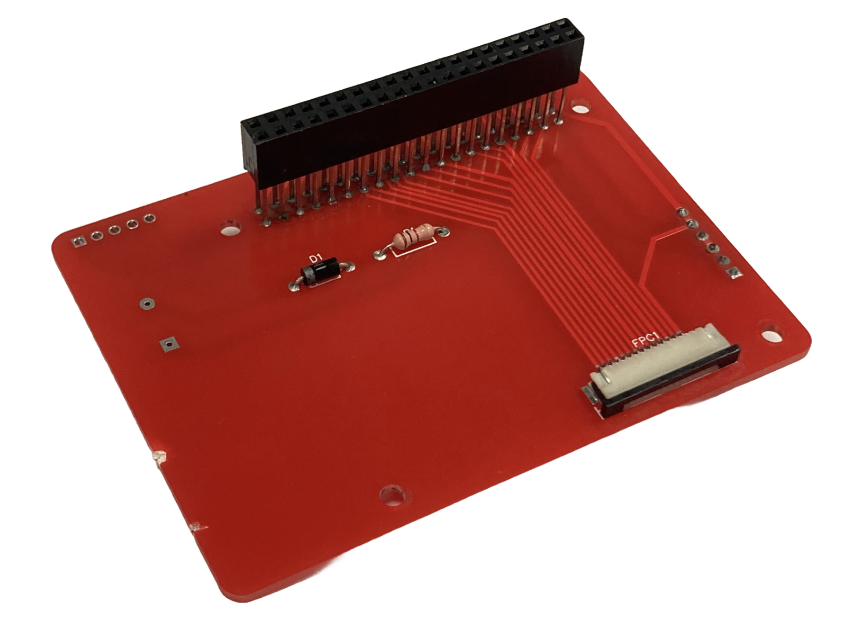
\includegraphics[width=0.5\textwidth]{Pictures/Pi_PCB_bottom.png}
    \caption{Pi PCB (bottom)}
    \label{fig:Pi_PCB_bottom}
  \end{minipage}
  \begin{minipage}{0.5\textwidth}
    \centering
    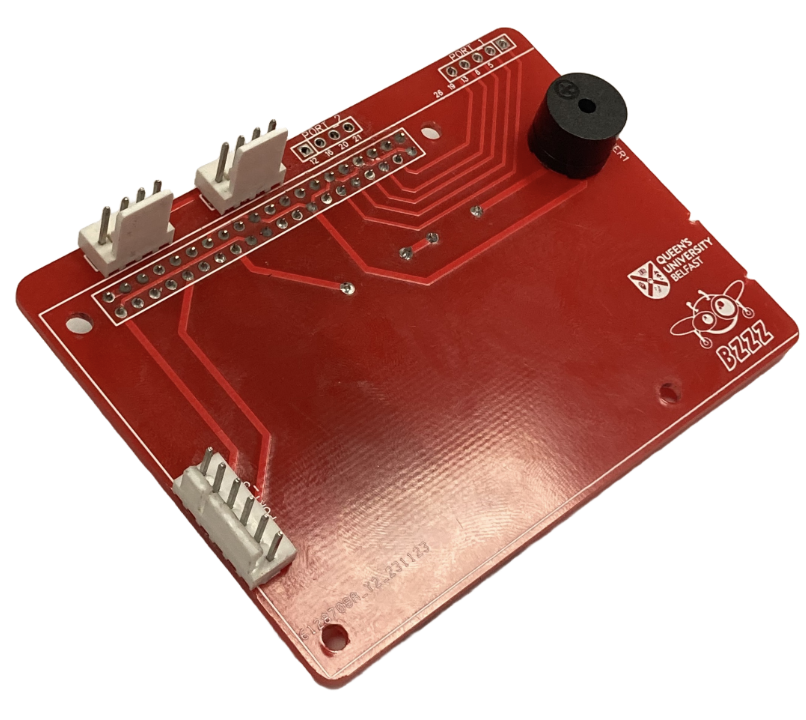
\includegraphics[width=0.5\textwidth]{Pictures/Pi_PCB_top.png}
    \caption{Pi PCB (top)}
    \label{fig:Pi_PCB_top}
  \end{minipage}
\end{figure}
\begin{figure}[H]
  \centering
  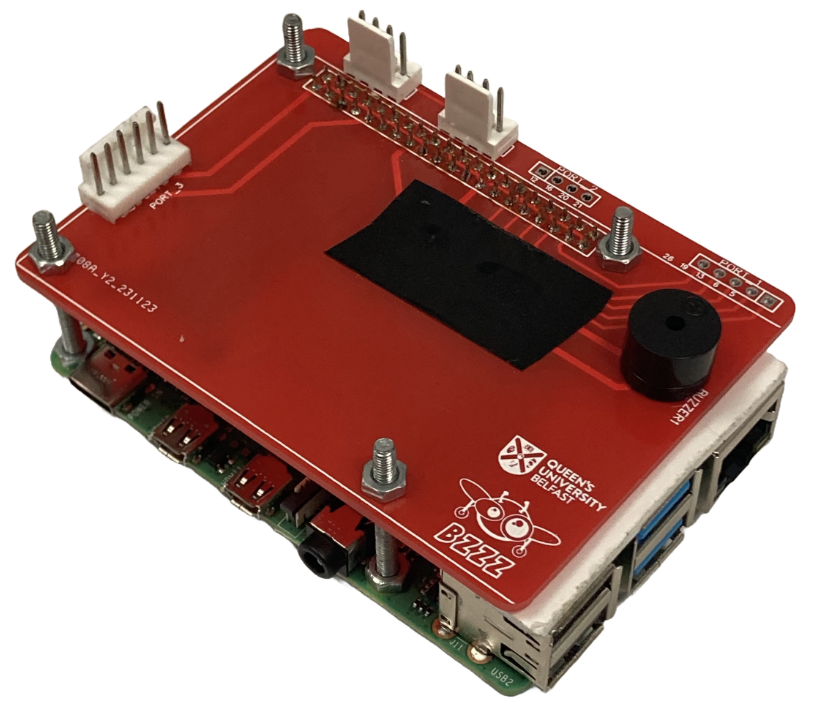
\includegraphics[width=0.35\textwidth]{Pictures/Pi_PCB_on_Pi.png}
  \caption{Pi PCB attached to Pi}
  \label{fig:Pi_PCB_on_Pi}
\end{figure}
The custom designed Raspberry Pi shield is shown in
figures:\ref{fig:Pi_PCB_bottom} and \ref{fig:Pi_PCB_top} The radio receiver is
connected to the Raspberry Pi GPIO via an SBUS connection in this circuit and
the Anemometer and GNSS connections via UART. The Raspberry Pi's I2C and UART
communication pins are linked to a IDC ribbon cable connector for communication
with the sensor PCB, see Section:\ref{sensorpcb}.

The mounting holes at the four corners of the PCB are used to fasten the board
to the Pi after it has been plugged into the Pi's GPIO pins. This is depicted in
Figure:\ref{fig:Pi_PCB_on_Pi}

\subsection{ESP PCB}
\begin{figure}[H]
  \centering
  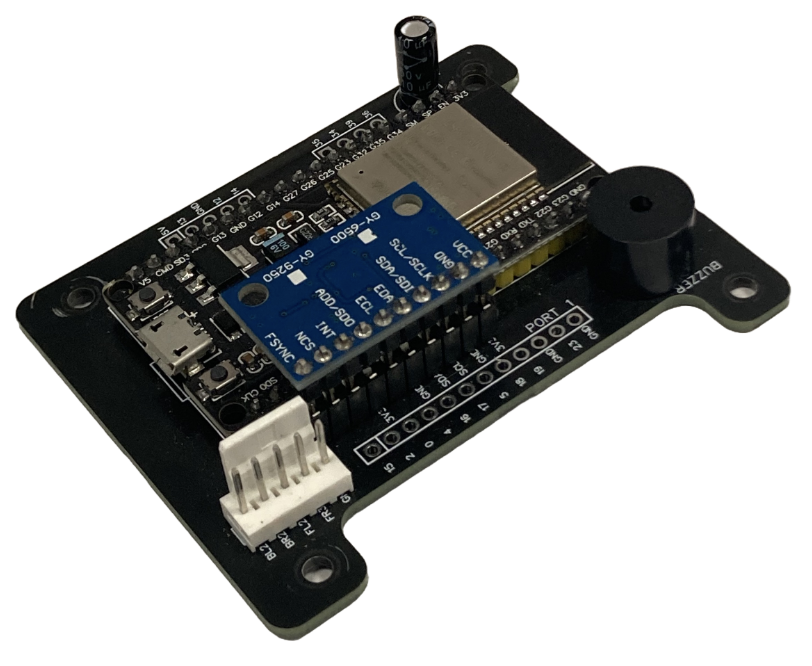
\includegraphics[width=0.35\textwidth]{Pictures/Esp_IMU_board.png}
  \caption{ESP32 PCB with IMU attached}
  \label{fig:Esp_IMU_PCB}
\end{figure}
The ESP shield is a custom designed PCD for electrical designs on the ESP32
WROOM board. All of the connections required to link the ESP and IMU via I2C are
included in the circuit. It additionally allows the ESP to connect to the ESCs
and a buzzer. The ESP shield is depicted above in Figure:\ref{fig:Esp_IMU_PCB}.

The ESP, the IMU, and the buzzer can all be accommodated on the board.
Furthermore, every unassigned pin is now connected to one of three ports; PORT
1, PORT 2, and PORT 3, respectively. Four mounting holes on the board line up
with the Pi's mounting holes, depicted in Figure:\ref{fig:flightController2}.

\begin{figure}[H]
  \centering
  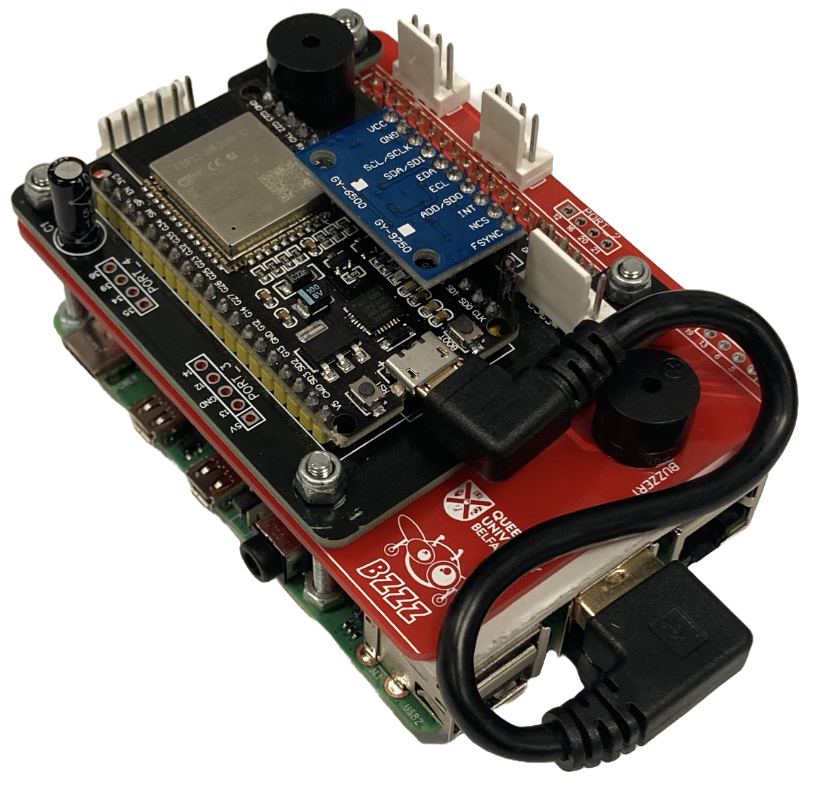
\includegraphics[width=0.35\textwidth]{Pictures/flight_controller.png}
  \caption{Flight controller}
  \label{fig:flightController2}
\end{figure}
After the flight controller is assembled, we have a powerful system that serves
as the basis for the quadcopter's functional abilities. The Raspberry Pi shield
guarantees reliable device interface thanks to its strategic placement of
connections to the radio receiver, GNSS and Anemometer. Essential GPIO pins
through an SBUS and an IDC ribbon cable connector for the ToF and Pressure
sensor (see Section:\ref{sensorpcb}). the ESP32 shield is carefully  designed to
fit both the ESP module and the MPU9250 IMU.For increased connectivity choices,
each unallocated pin is systematically attached to one of the three available
ports (PORT 1, PORT 2, and PORT 3). The USB connection between the Raspberry Pi
and the ESP32 completes this assembly and provides a dependable, fast
communication channel that is essential for the interchange of control and
sensor data.

\subsection{Sensor PCB}\label{sensorpcb}
\begin{figure}[H]
  \centering
  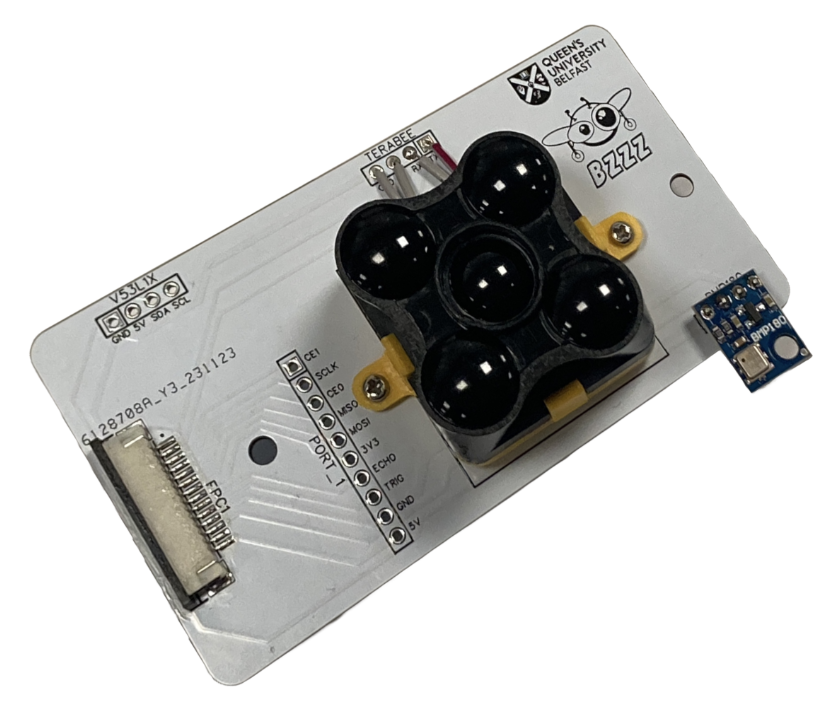
\includegraphics[width=0.3\textwidth]{Pictures/sensorpcb.png}
  \caption{Sensor PCB, including ToF and Barometer sensors}
  \label{fig:sensorpcb}
\end{figure}
The sensor PCB is designed to be installed at the quadcopter's base attached to
the baseplate. By ensuring that the Time-of-Flight (ToF) and Barometer sensors
are exposed to the environment without obstruction, a crucial aspect for
accurate measurements, this placement optimises their operation. The sensors are
positioned strategically to reduce interference from other electronics and to
provide a steady platform for the correct collection of altitude data, which is
essential to the flight control system. The method of establishing communication
between the Raspberry Pi and the Sensor PCB involves attaching a Flexible Flat
Cable (FFC) to the IDC ribbon cable connector. The ToF sensor is attached via
bolts and the barometer is soldered on.

\subsection{Power Distribution PCB}
\begin{figure}[H]
  \centering
  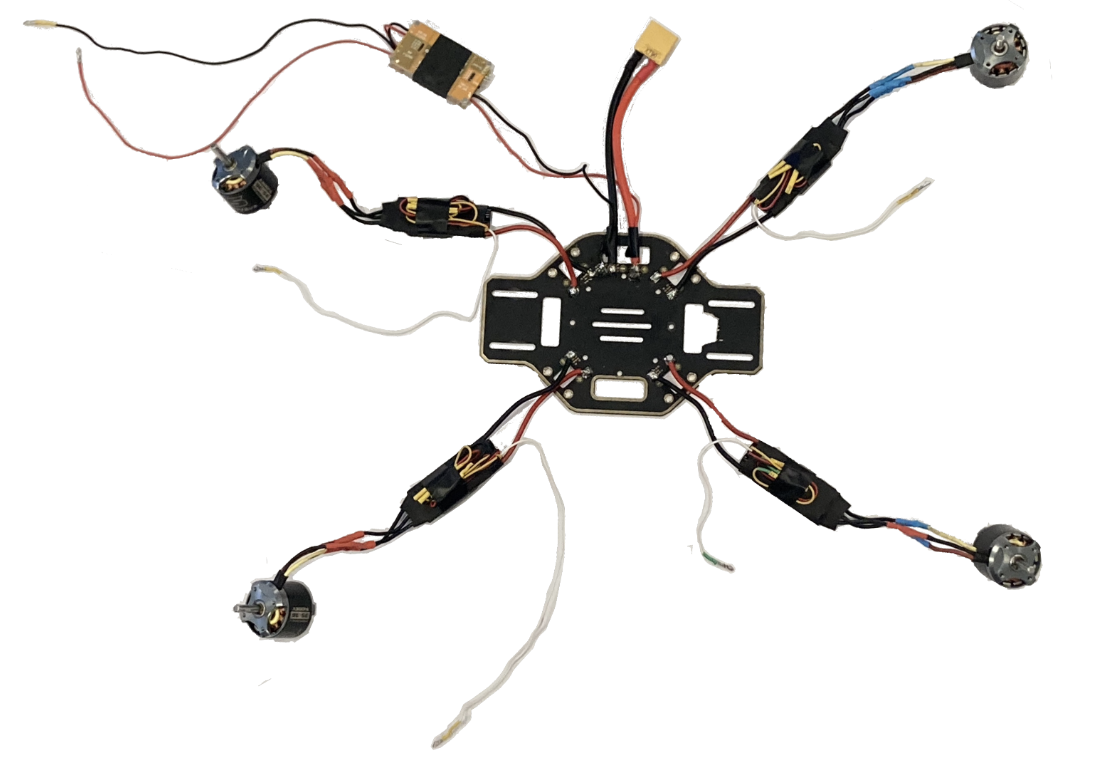
\includegraphics[width=0.5\textwidth]{Pictures/power_distribution_and_escs.png}
  \caption{Power distribution board}
  \label{fig:power_distribution}
\end{figure}
The power distribution PCB depicted above in Figure:\ref{fig:power_distribution}
is the central hub for distributing powers across the quadcopter. Each
Electronic Speed Controller (ESC) is connected to the PDB, which receives power
from the main battery. The ESCs then regulate the power to the motors, adjusting
speed and rotation based on the control signals received, via PWM (Pulse Width
Modulation) from the flight controller.

The ESCs are essential for supplying the controlled, variable power required for
the exact movements of the quadcopter. They are coupled to their respective
motors. The quadcopter's manoeuvrability is made possible by the ESCs, which
make sure the motors react appropriately to inputs from the flight controller.
The PDB guarantees that all the electronic components receive the power they
require.

Stable power delivery to the flight controller is ensured by the voltage
regulator, which is essential for its computational tasks and stability
functions. It powers vital navigation and control systems, such as the GNSS
module, IMU, Anemometer, ToF sensor and Barometer, by converting the battery's
fluctuating voltage to a constant level, which helps the quadcopter fly
precisely and steadily.


\chapter{Software}                            
This project’s code is all located in one repository on
\href{https://github.com/QUB-ASL/bzzz}{GitHub}. The purpose of a central
platform for version control and communication is served by the repository. The
extensive documentation to help developers understand and contribute to the
project is available in the repository.  Its methodical arrangement makes it
simple to navigate through a variety of components, such as control systems,
Kalman filters, and sensor integration

My project involvement has also seen me contribute to the veatures of features
that allowed the interpretation of GNSS data that translates the satellite
signals into usable location information for the drone. I interpreted barometer
data that gave the altitude from pressure readings, Kalman filter design. I took
charge of setting up all sensors in the system paving the way for sensor fusion
and data amalgamation

I gave clear explanations and usage guidelines for our Kalman filter, to make
the system easier to understand and use, setting the ground for further
enhancements. I have accomplished the development of the Kalman filter itself by
using simulators I found the optimal tuning valuses for performance of the
Kalman filter in the Altitude and Position control tasks. I designed a PID
controller for the Positioning control and a PD controller for the altitude
control with the Kalman filter for the sensor fusion, determining accurate
funcionality was achieved through simulation design. This underscores the
projects dedication to responsive control mechanisms.

These contributions demonstrate my involvement, with the project and dedication
to enhancing the capabilities of this system while aligning with my project
objectives.

\section{Main Loop}
\begin{figure}[H]
  \centering
  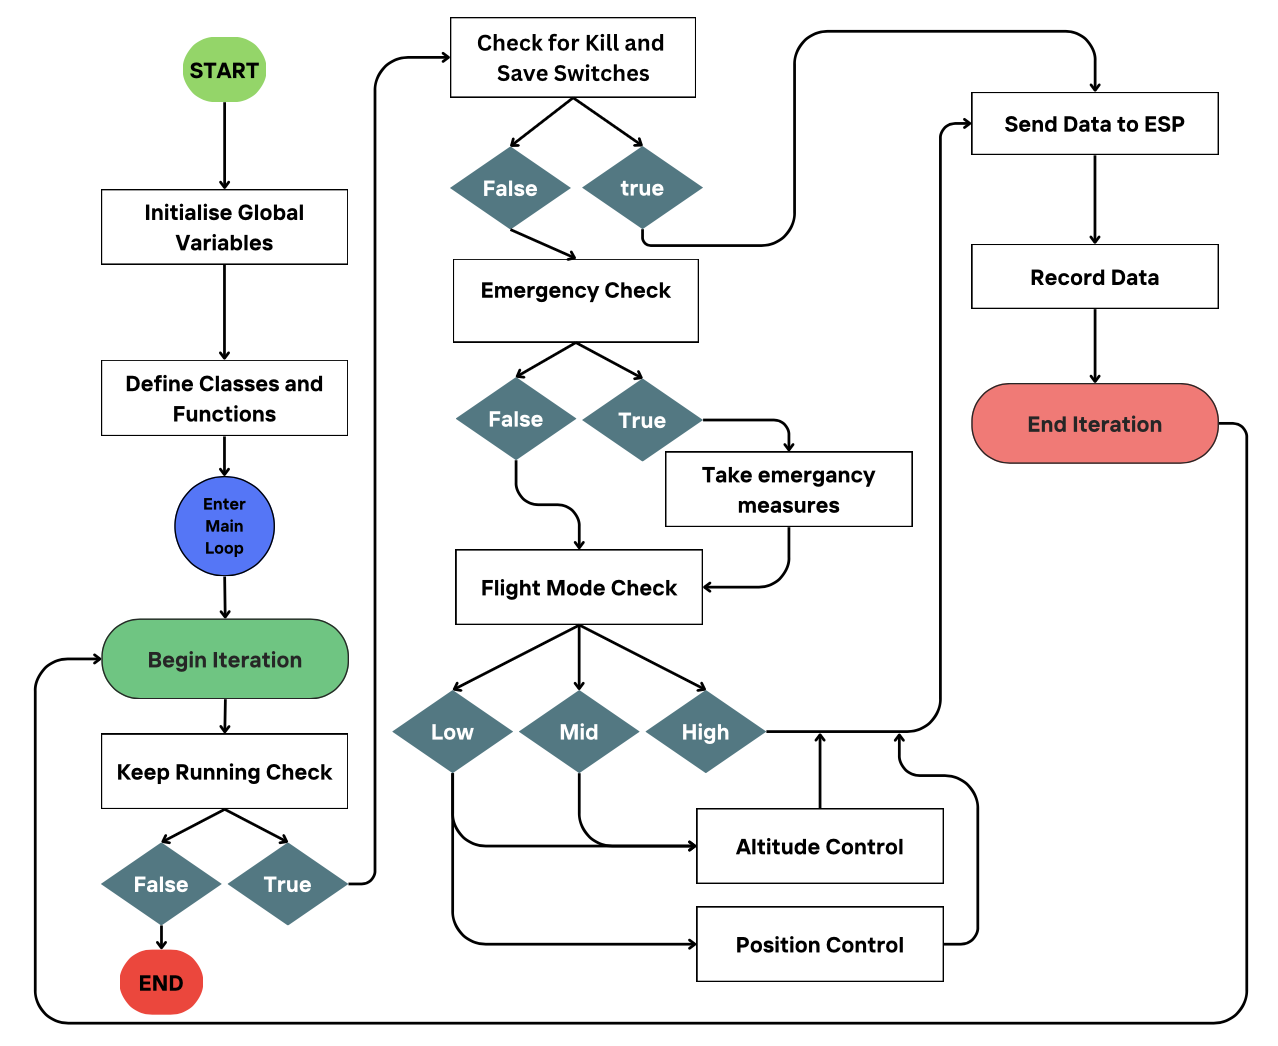
\includegraphics[width=0.8\textwidth]{Pictures/main_loop_flowchart.png}
  \caption{Main loop flowchart}
  \label{fig:main_loop_flowchart}
\end{figure}

The drone control programme starts by configuring the necessary runtime
environment, which includes initialising global variables and parameter
configurations that are essential for flying operations. During this stage, the
system loads vital values from a preset constants module, like the minimum
altitude required for altitude hold and sensor calibration data. Furthermore,
instances of the DataLogger and AltitudeHoldKalmanFilter classes are brought
in, in order to offer real-time data logging and altitude estimate
capabilities.

Once all necessary classes and functions have been defined, the system enters
its main operating loop. The constant processing of actuator commands and sensor
readings forms the core of the control system, represented by this loop. At the
beginning of each iteration, a conditional flag that indicates whether the loop
should continue is checked. The 'Keep Running Check' looks for unexpected
behaviour or outside orders to halt processes. In order to make sure the
software can seamlessly exit the loop when necessary, it verifies user inputs
from the RC and analyses the present state of the system.

The 'kill' and 'save' switches in the RC (Remote Control) class are checked as
part of the flight control logic. In unwanted situations, it enables the user to
command the system to store flight data records or to stop the entire flight. In
the event that the quadcopter loses communication with the remote controller or
is 'killed' above a predetermined height, the software initiates a 'Emergency
Check' to determine whether prompt safety measures are required. These
measurements are based on real-time sensor data from the Time of Flight sensor.
To put emergency responses into action, utilise the take emergency measure
function. The likelihood of the quadcopter crashing is decreased by taking
various actions, such as adjusting the throttle for a controlled landing,
depending on how serious the issue is.

In addition, the control system carries out a 'Flight Mode Check', in which it
uses the input from the RC class to determine the proper control response, such
as position control or altitude hold. if the drone is in the proper state ,the
AltitudeController and PositionController classes are used to calculate the
necessary control signals based on the feedback from location and altitude
sensors. These particular controllers are a crucial component of an intricate PD
and PID systems that dynamically regulates propulsion on all axes to allow the
drone to fly in the correct direction.

Communication with peripheral modules are handled by the EspBridge class, which
serializes control and telemetry data and transmits it to the ESP module for
further communication or processing. Moreover, the data obtained during the
flight is stored using the DataLogger class that records time-stamped sensor
readings alongside the control commands. This will be utilised as a black box
record that is critical for post-flight assessment and provides invaluable
analysis for enhancements.

The classes demonstrate that the system was developed with concurrent operation
in mind. By handling sensor data acquisition in parallel to the primary control
loop, the ToF, pressure sensor and Gnss classes reduce the amount of influence
latency has on controller responsiveness. To ensure the integrity of sensor data
required for control decisions and to avoid data races, these classes employ
thread locks to synchronise access to shared resources. In addition, the
DataLogger class was crafted such that the act of recording data has no effect
on the main control loop's performance.

In conclusion, a well-designed set of checks and controls throughout the
quadcopters control system architecture allows for a secure and stable
operation. The quadcopters software conducts precision flight control yet
maintains an unwavering interest in safety through constant real-time monitoring
and management of contingencies. The multi-threaded architecture and
asynchronous processing of sensor data gathering highlight the system's
efficiency in a real-time setting, indicating a system prepared to withstand the
demanding requirements of aerial operations.

\section{Sensor Data Aqusition}
\begin{figure}[H]
  \centering
  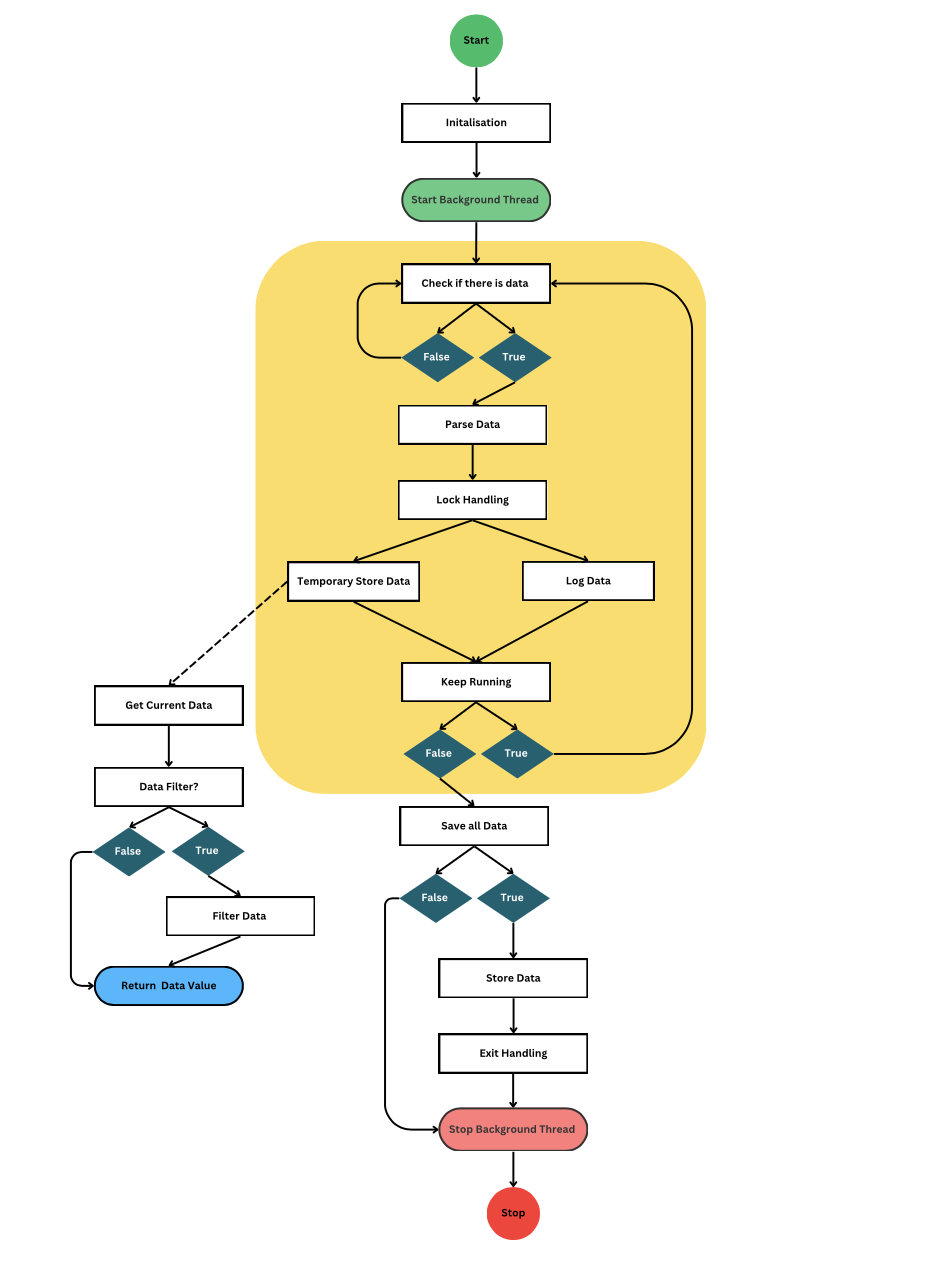
\includegraphics[width=0.8\textwidth]{Pictures/sensor_flowchart.png}
  \caption{Sensor flowchart}
  \label{fig:Sensor_flowchart}
\end{figure}
The technical execution of the sensor data processing system begins in the
initialization phase: it involves configuring global variables and creating a
framework for data collecting. The sensor class's are set up in this phase to
specify the window length for data processing, establish the serial channel and
baud rate for transmission, and, if necessary, instantiate the median filter and
data logger. 

The system launches a background thread following the successful completion of
the initialization step. This is essential to the system's capacity to carry out
asynchronous operations. The thread's job is to read data from the sensor at all
times, working autonomously and without interfering with or disrupting the main
control loop. 

The system ensures that data access is thread-safe by applying a lock mechanism
the system defines a lock state, which prohibits simultaneous write/read
operations that can lead to data corruption. Its key action in the control loop
is to periodically check the serial buffer for new data. If new data are
identified, the raw data is read, processed, and converted into a format that
can be used to describe the sensor measurements like distance/altitude. The
parsed data is temporarily stored in an array, maintaining the synchronization
guaranteed by the lock to ensure that multi-threaded operations always preserve
data consistency. 

Another critical function in the control loop is data logging. If active, the
drone's sensory inputs create a permanent record by adding each sensor reading,
which is perfectly timestamped, to a log file in csv format. This data is
critical for post-flight analysis. Furthermore, a conditional filter check is
appended to decide if it is necessary to perform additional processing on the
newly acquired data to reduce noise or outliers. When filtering is necessary, ta
Median Filter analyses the data that has been stored and returns a refined value
that the system may use.

In the main loop, a 'Keep Running' check determines whether or not the system
should keep running. When a user tries to end a flight, such as when they
activate the 'kill' or 'save' switches, the code will be broken out of this
loop. In the event that the exit condition is satisfied, the system immediately
saves all of the gathered data in order to prevent data loss. This safeguard
comes before the organised method of leaving, which includes terminating the
background thread. This methodical exit procedure guarantees a secure
termination by ensuring that all tasks are completed smoothly, that the data is
saved, and that the system resources are freed.

The system enters a halt state and stops all operations in the last phase. The
program’s execution thread cycles comes to an end with this step. Therefore,
mentaining data safety when terminating the quadcopter.


\chapter{Tests}\label{tests}

\section{GNSS rover rodule test, with correction Vs
without}\label{GNSS_rover_module}
\begin{figure}[H]
  \centering
  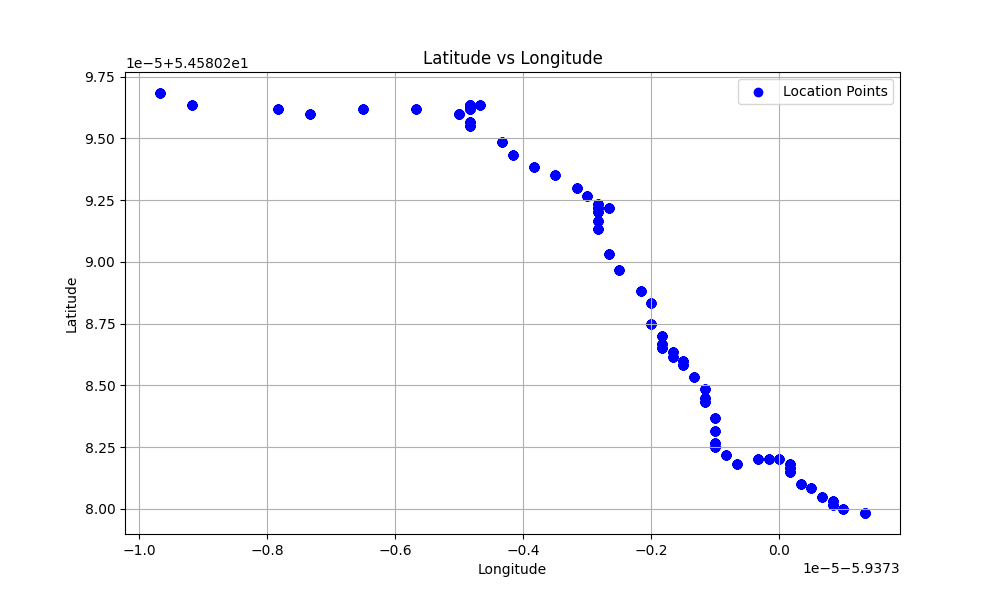
\includegraphics[width=0.8\textwidth]{Pictures/GNSS_no_RTK.png}
  \caption{GNSS readings without the use of RTK corrections form the base station}
  \label{fig:GNSS_no_RTK}
\end{figure}

\begin{figure}[H]
  \centering
  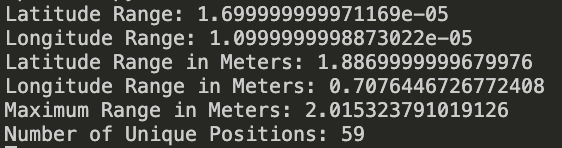
\includegraphics[width=0.5\textwidth]{Pictures/GNSS_data_no_correction.png}
  \caption{GNSS Percesion Data (Without corrections)}
  \label{fig:GNSS_data_no_RTK}
\end{figure}
In the figures above, Figure:\ref{fig:GNSS_no_RTK} and
Figure:\ref{fig:GNSS_data_no_RTK} represent the GNSS latitude and longitude
recorded while the module remained in a fixed position. The purpose of this
setup was to calculate the overall precision of our GNSS module without the
correction data streaming from the base station.

From the above graph in Figure:\ref{fig:GNSS_no_RTK} we can see that the
recorded longitude and latitide points are drifting. Ideally, when a GNSS module
is fixed in one position, it would be expected that the recorded latitude and
longitude data points to cluster tightly around a single coordinate pair,
indicating a high level of precision. However this is not the case as the spread
of data points seen here suggests a certain level of positional inaccuracy, this
is due to the fact that the module is not availing of the RTK correction stream
from the GNSS base station we have set up. 

Figure:\ref{fig:GNSS_data_no_RTK} shows a terminal output from the python code
written to summerise the data recorded. From this we can see that the range of
values of longitude and latitude readings, converted to meters are, 1.887m
(3.d.p) and  0.708m (3.d.p). Next the overall max and min points on the graph
are calclulated using Pythagorean theorem showing that the readings span over
2.015m (3.d.p) accross 59 readings.

In Conclusion, the test results show that,the accuracy of GNSS data is limited
and are not be suitable for applications that require high precision. The
variations in data points and observed drift indicate that the GNSS modules
accuracy fluctuates, potentially affecting its reliability when used in position
control on the quadcopter. With a dispersion of 2.015 meters across 59 readings
it is clear that using RTK corrections is essential for getting more accurate
data. While the GNSS module offers location information it falls short in
meeting the precision requirements whitch are needed for accurate position
control.


\begin{figure}[H]
  \centering
  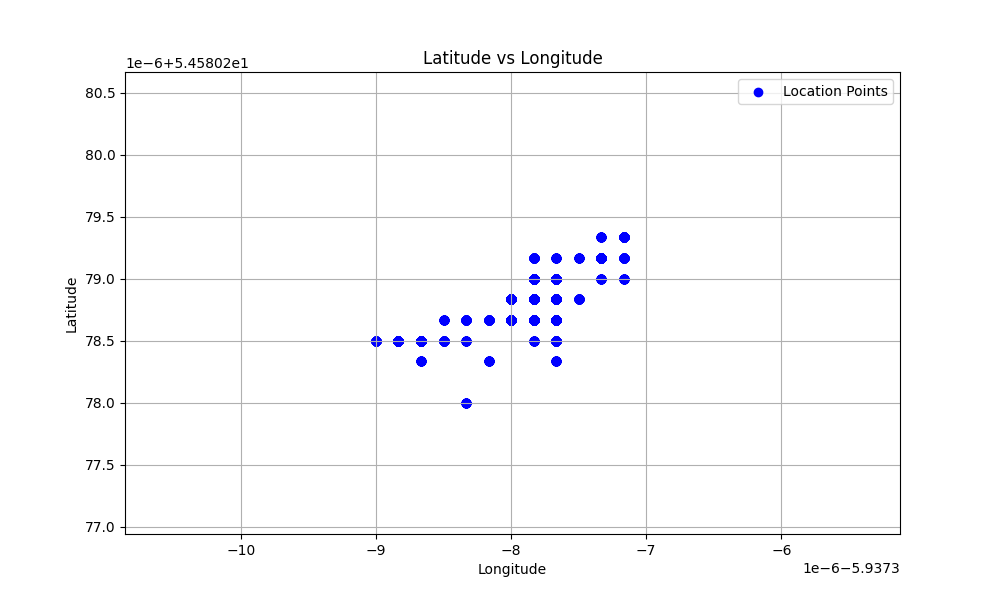
\includegraphics[width=0.8\textwidth]{Pictures/GNSS_RTK.png}
  \caption{GNSS readings with the use of RTK corrections form the base station}
  \label{fig:GNSS_RTK}
\end{figure}

\begin{figure}[H]
  \centering
  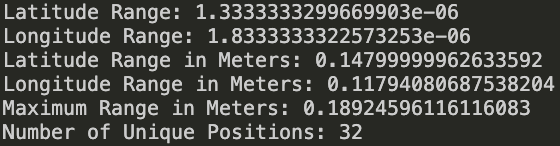
\includegraphics[width=0.5\textwidth]{Pictures/GNSS_data_correction.png}
  \caption{GNSS Percesion Data (With corrections)}
  \label{fig:GNSS_data_RTK}
\end{figure}

In the figures above, Figure:\ref{fig:GNSS_RTK} and
Figure:\ref{fig:GNSS_data_RTK} represent the GNSS latitude and longitude
recorded while the module remained in a fixed position. The purpose of this
setup was to calculate the overall precision of our GNSS module without the
correction data streaming from the base station.

From the above graph in Figure:\ref{fig:GNSS_RTK} we can see that the recorded
longitude and latitide points are in a distinct cluster. Due to the fact that
RTK corrections have now been streamed from the base station there is less
variation in readings, indicating a high level of precision.

Figure:\ref{fig:GNSS_data_no_RTK} shows a terminal output from the python code
written to summerise the data recorded. From this we can see that the range of
values of longitude and latitude readings, converted to meters are, 0.148m
(3.d.p) and  0.118m (3.d.p). Next the overall max and min points on the graph
are calclulated using Pythagorean theorem showing that the readings span over
0.189m (3.d.p) accross 32 readings.

In conclusion the use of RTK corrections has proven vary useful, shocasing
values of high percision, which is needed for position control on the
quadcopter. There is little variation in data points with a dispersion of 0.189
meters across 59 readings, when copared to 2.015 meters in the test above it is
undeniable the significant enhancement in accuracy achieved through ustalizing
RTK corrections. 

\section{Testing of Kalman filter}
\begin{figure}[H]
  \centering
  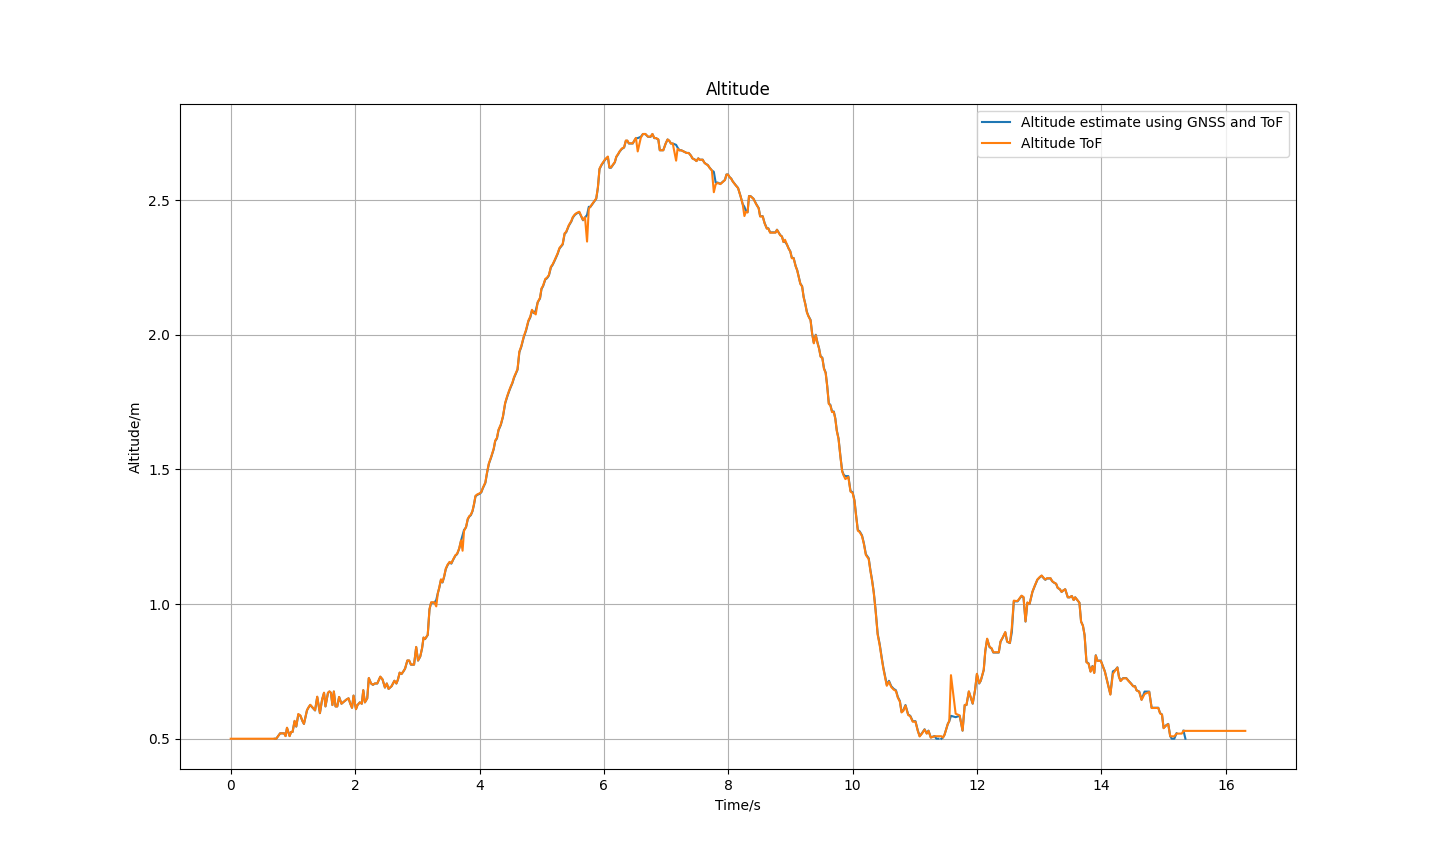
\includegraphics[width=0.8\textwidth]{Pictures/Altitude_with_GNSS.png}
  \caption{Time of Flight sensor vs sensor fused Kalman filter with GPS and ToF data}
  \label{fig:Kalman_filter_test}
\end{figure}

\begin{figure}[H]
  \centering
  \includegraphics[width=0.8\textwidth]{Pictures/Altitude_with_GNSS_zoomed.png}
  \caption{Time of Flight sensor vs sensor fused Kalman filter with GPS and ToF data zoomed}
  \label{fig:Kalman_filter_test_zoomed}
\end{figure}
In this test the quadcopter was briefly flown in order to test the kalman filter and how well it filters noisey data when compared to using the ToF sensor by itself.

From Figures:\ref{fig:Kalman_filter_test} and \ref{fig:Kalman_filter_test_zoomed} we can see that the kallman filter does a good job at filtering out the noisey data smoothing out the curve of altitude measurments.

This is especially usefull when it comes to flying over uneven terain such as long grass where using the ToF sensor alone will introduce inacuracys in the altitude measurements.

\section{Testing initial estimate for \(\alpha_0\) and \(\beta_0\)}
  \begin{figure}[h]
    \centering
    \begin{tikzpicture}
      \begin{axis}[ width= 4in, height=2in, scale only axis, ylabel={Lift (g)},
          xlabel={Throttle reference (\%)}, xmajorgrids, ymajorgrids, ylabel
          near ticks, xmin=10, xmax=40, ymin=0, ymax=2500, legend columns=1,
          legend style={fill=white, fill opacity=0.4, text opacity=1,
          font=\scriptsize}, legend style={at={(axis cs:10.5,2450)},anchor=north
          west}, legend cell align={left}, ]

        \addplot[mark=x, blue, only marks, line width=1.2pt]
        table [x=throttle_percentage, y=weight_decrease, col sep=comma]
          {Data/1045_full.csv}; \addlegendentry{Full battery ($R^2=99.99\%$)};

        \addplot[mark=none, blue!50, only marks, line width=1.2pt, mark=x]
        table [x=throttle_percentage, y=weight_decrease, col sep=comma]
          {Data/1045_low.csv}; \addlegendentry{Low battery ($R^2=90.1\%$)};


        \addplot[domain=0:50, blue, dashed]
        table [x=throttle_percentage, y = {create col/linear regression =
          {y=weight_decrease}}, col sep=comma] {Data/1045_full.csv}; \addplot[no
          marks, blue, dashed,
          domain=0:50]{\pgfplotstableregressiona*x+\pgfplotstableregressionb};

        \addplot[domain=0:50, blue!50, dashed]
        table [x=throttle_percentage, y = {create col/linear regression =
          {y=weight_decrease}}, col sep=comma] {Data/1045_low.csv}; \addplot[no
          marks, blue!50, dashed,
          domain=0:50]{\pgfplotstableregressiona*x+\pgfplotstableregressionb};

      \end{axis}
    \end{tikzpicture}
    \caption{Static lift (g) plotted against throttle reference (\%).}
    \label{fig:liftpwm_test}
  \end{figure}

The quadcopter was placed on digital scales ontop of a platform to minnimize
ground effect, and the lift (in g) was measured for different values of
\(\tau\). The experimental results are shown in Figure:\ref{fig:liftpwm_test},
the graph shows a clear linear relationship between the throttle reference and
the static lift produced by the quadcopter. There are two sets of data
represented by two different linear fits: one for when the battery is full and
another for when the battery is low.

From the trendlines in the graph the derived model for the lifting force is
\(F_{\rm prop} = \alpha_0 \tau + \beta_0\), where $\alpha_0>0$ and $\beta_0<0$
are constants, which depend on the level of charge of the battery.

\begin{itemize}
  \item \textbf{Full Battery}: The graph shows that the quadcopter has a
    relatively constant lift force across various throttle references when the
    battery is fully charged. The high \(R^2\) value of 99.99\% which indicates
    an almost perfect linear correlation, is evidence of this. When the battery
    is fully charged, the slope of this line would be \(\alpha_0\) and where the
    line intersects the y-axis (lift) is \(\beta_0\).
  \item \textbf{Low Battery}: The slope of the line becomes less steep when the
    battery is low, indicating that \(\alpha_0\) is smaller when the battery is
    low than when it is full. Additionally, the \(R^2\) value is lower (90.1\%),
    indicating a less consistent relationship that may be caused by variations
    in battery performance as the charge decreases. again where the line
    intersects the y-axis (lift) is \(\beta_0\).
\end{itemize}
In conclusion, the values for \(\alpha_0\) and \(\beta_0\) were found to be 8654
and -797.67 respectively. These values were then used in
equations:\ref{eq:alpha} and \ref{eq:beta} for deriving the initial values for
\(\alpha\) and \(\beta\) in the Kalman filter.

\section{Altitude control}\label{altitude_cotrol_tests}
\subsection*{Altitude control whilst quadcopter is static}
\begin{figure}[H]
  \centering
  \includegraphics[width=0.7\textwidth]{Pictures/Altitude_hold_indoors.png}
  \caption{Altitude control whilst quadcopter has little horizontal movement}
  \label{fig:Altitude_control_no_movement_altitude}
\end{figure}
In this test shown in Figure:\ref{fig:Altitude_control_no_movement_altitude} tookplace indoors using the Time of Flight (ToF) sensor only, the
Quadcopter is taken off in manual flight mode as usual once a steady altitude
was found using the throttle on the remote, the altitude control mode was
initalised using the RC. The altitude trimmer was then used to lower the
altitude refferance until it was low enough to land in manual mode. In the graph
the Green line represents the true altitude from the ToF sensor, the Orange line represents the
refferance altitude. 
From the above graph we can see that the quadcopter performes well in a
controlled osolation around the refferance point of \(\pm10\) centimeters
thought. The quadcopter behavior demonstrated a well tuned PD controller with a
P gain of 0.5 and a D gain of 0.07, this control proved impressive as it was
able to follow the refferance altitude down as the trimmer was decrecing,
mentaining the same accuracy as before in a consistant altitude. The lack of
spikes in velocities seen in the altitude control portion of the graph proves
impressive when compared to manual mode, showcasing the its persise control over
the quadcopter.

\begin{figure}[H]
  \centering
  \includegraphics[width=0.7\textwidth]{Pictures/Throttle_Altitude_hold_indoors.png}
  \caption{Throttle measurments in Altitude control mode whilst quadcopter has little horizontal movement}
  \label{fig:Altitude_control_no_movement_Throttle}
\end{figure}

The graph above (Figure:\ref{fig:Altitude_control_no_movement_Throttle}) depicts the throttle percentage readings against time. The graphs shows continuously smooth throttle changes when the altitude refrence is not being changed, followed by a slight osolation when the refferance is lowered gradually. This inaccuracy is then mitigated as the altitude converges back on the refferance altitude.

\begin{figure}[H]
  \centering
  \includegraphics[width=0.7\textwidth]{Pictures/Velocity_Altitude_hold_indoors.png}
  \caption{Velocity measurments in Altitude control mode whilst quadcopter has little horizontal movement}
  \label{fig:Altitude_control_no_movement_Velocity}
\end{figure}
When analysing the velocity graph in the test (Figure:\ref{fig:Altitude_control_no_movement_Velocity}) it can be seen that the velocity of the quadcopter is emediatly smoothed when altitude control mode has been initalised around the 10 second mark. The velocity of the quadcopter continues to stay smooth until the altitude reffernce is lowered causing some inaccuracy followed by a further conversion velosity as the true altitude gets closer to the refferance altitude.

In conclusion the quadcopter's performance in the altitude control mode, as
shown in this test, was deemed exceptional. The altitude accuracy of \(\pm10\)
centimetres from the reference altitude shows that the system is capable of
exceptional control usiing a PD controller even when the refferance altitude is
being altered. Hense this test proves the quadcopter to be a good soloution for
many different aplications of arial control such as, photography, surveying and
search and rescue. 

Furthermore, It could potentially be further improved with additional
calibration of the P and D values in the controller, this will take further time
and testing. 


\subsection*{Quadcopter moving whilst in altitude control mode}
\begin{figure}[H]
    \centering
    \includegraphics[width=0.6\textwidth]{Pictures/Altitude_hold_test_moving.png}
    \captionsetup{justification=centering}
    \caption{Altitude control test \\ whilst quadcopter is moving}
    \label{fig:Altitude_hold_test_moving}
\end{figure}
\begin{figure}[H]
    \centering
    \includegraphics[width=0.6\textwidth]{Pictures/GNSS_Altitude_hold_test_moving.png}
    \captionsetup{justification=centering}
    \caption{GNSS Data from Altitude \\ Control flight path}
    \label{fig:GNSS_Altitude_hold_test_moving_gps}
\end{figure}
In this test, the quadcopter was taken off and landed as normal. During the
flight the altitude control feature was initalised on the quadcopter and flown
the quadcopter, flying in a radius of around 10m, shown in
Figure:\ref{fig:GNSS_Altitude_hold_test_moving_gps}.

Figure:\ref{fig:Altitude_hold_test_moving} illustrates the quadcopters
altitude in orange, refferance altitude in green, throttle signal in red and the
velocity in blue.

It is crucial to take into account the circumstances and external influences
that might have affected the recorded outcomes when assessing how well the
quadcopter's altitude control capability performed. The quadcopter flew with an
altitude accuracy of about \(\pm30\) centimetres from the reference altitude of
3.1m, as stated in the test description. This indicates a reasonably stable
performance while operating in the altitude control mode. This degree of
accuracy is impressive, especially in light of the difficulties caused by
outside variables like strong winds and the dynamics of the quadcopter's motion.

As the test continues the altitude trimmer on the side of the remote was
increased, this in turn gradually increases the refferance altitude. From the
graph we can see that the quadcopter successfully reacted to this change in
refferance, furthermore showcasing the quadcopers control algorithms abilities.

The disparity in altitude control, as seen in
Figure:\ref{fig:Altitude_hold_test_moving},can be linked to the high wind
velocity that was present throughout the test. Because wind exerts unpredictable
forces on the quadcopter, it can create significant unpredictability in altitude
control, making it more difficult to keep a steady altitude.

Furthermore, altitude control may become even more challenging due to the
quadcopter's movement, particularly when it involves pitch and roll changes. A
forward/backword pitch or left/right roll can cause a drop in altitude if it
isn't corrected for by increasing the throttle, as
Figure:\ref{fig:ToF_altitude_error} shows bellow. This is due to the fact
that when the quadcopter is tilted forward or sidewards for movement, it directs
some of the thrust horizontally, thereby reducing the vertical thrust component
that counteracts gravity. In such cases, in order to maintain the required
height, the altitude control system has to dynamically adjust the throttle which
can cause the controler to osolate between movements. In order to fix this problem the relevent pitch and roll angles should be parsed from the IMU, these angles should them be used in the basic trigonometry equation \(a = recorded_{altitude} \cdot \cos(\theta)\) where a is the true altitude and \(\theta\) is the recorded angle from the IMU.

\begin{figure}[H]
  \centering
  \includegraphics[width=0.9\textwidth]{Pictures/ToF_altitude_error.png}
  \caption{Moving quadcopter causing an decrease in altitude if throttle percentage is kept the same}
  \label{fig:ToF_altitude_error}
\end{figure}

In light of the operational and environmental difficulties encountered, the
quadcopter's performance in the altitude control mode, as proven in this test,
was deemed good. Even if there is still space for development, the altitude
accuracy of 0.6 metres from the reference altitude shows that the system is
capable of handling external elements like wind and movement dynamics. It can be
further with additional calibration of the P and D values in the controller. The
altitude control capability will need to be continuously improved and tested in
a variety of scenarios in order to function more precisely and consistently.


\chapter{Reflection on progress}
\section{Time analysis}
In the Time analysis segrment, systematic analysis of the various aspects of the
bzzz project, detailing the duration and sequencing of the developmental phases,
implementation, and testing of the bzzz quadcopter. The meticulous break down of
time alocation for each task in the project, highlighting efficiency gains and
bottlenecks encountered.

Below in figures:\ref{fig:gantt_chart} and \ref{fig:gantt_chart_key} is the
gantt chart and key provided in the Intrim report:
\begin{figure}[H]
  \centering
  \rotatebox{-90}{\includegraphics[width=1.2\textwidth]{Pictures/gantt_chart.png}}
  \caption{Gantt chart}
  \label{fig:gantt_chart}
\end{figure}
\begin{figure}[H]
  \centering
  \includegraphics[width=0.2\textwidth]{Pictures/Gantt_chart_key.png}
  \caption{Gantt chart key}
  \label{fig:gantt_chart_key}
\end{figure}

\subsection*{Steps within time constraints}
The parsing of GNSS data aswell as testing the code was a notable sucess, our
results demonstrated the codes ability to efficiently managed to extract and
interpret the GNSS data streams using multi threading, parsing Latitude,
Longatude and  Altitude data, which are crucial for the quadcopter's
navigational systems. The sucess in this area was due to the extensive resurch
that was done in GNSS data strings prior to writing the code.

The GNSS rover module testing proved to be a strong point, offering insightful
information on the system's performance and capabilities in real-world
scenarios. A number of successful trials that verified the module's
functionality and reliability for more integration with the UAV system were
made possible by the well-organized testing processes.

Controller research also progressed within the alocated time constraints,
exploring various control strategies that could be applied to the bzzz
quadcopter. Due to this extensive resurch it was determined that a PD controller
for altitude control and a PID controller for position control was most
applicable. The derived plan from the resurch pathed the way for a quick
turnaround when it came to simulating the controller. 

Finally, designing simulations for the kalman filter progressed well, this was
due to the fact that extensive documentation was written prior to designing
these simulations. This documentation layed the groundwork for simulation
implementation providing great results from the get go meaning that little
tuning was needed, allowing for a quick turn around. 

\subsection*{Steps outside time constraints}
The Design of the kalman filter documentation percisted chalanges, taking longer
than expected. The complexity of the mathematical modeling required a more
extensive developmental phase to ensure the filter's accuracy and reliability
when it came to making simulations and overall implementation. On the otehr hand
the estended time spent writing the detailed documentation on the filter was
made up for when designing simulations and overall implementation as it paved
the way for these processes. 

The decision to implement a base station introduced unexpected complexities into
the system architecture. This ment having to do further research into
calibration, figuring out a way to brodcast the correctionn data from the base
station to the rover module, designing a water ressistant casing and finally the
design of the station that allowed for portability. 

Testing setbacks for altitude control were encountered due to unfavorable
weather conditions and an unfortunate incident of crashing. These external
factors meant that this process to longer than anticipated.

Lastly, the PD control implementation for altitude control faced hurdles. The
iterative process of tuning the PD parameters to achieve the desired level of
control and stability took additional time. Although the simulations provided
promising results they were not directly transferable to real life conditions
due to several factors such as weight and enviormental conditions.

\section{Objective analysis}
Upon starting this project objectives were layed out as well as the learning
outcomes, as seen below, 
\subsection*{Objectives}
\begin{enumerate}
  \item To design, implement and test a Kalman filter to estimate the (x, y, z)-
  position and the heading of the quadcopter using information from the IMU, the
  altimeter, and a GPS module.
  \item To design, implement and test a control system for loitering.
  \item To perform certain hardware tasks (proper mounting and connection of the
  GPS module to the on-board Raspberry Pi)
  \item To perform experiments and record flight data
\end{enumerate}

\subsection*{Learning Outcomes}
\begin{enumerate}
  \item Have mastered the theory of LQR and Kalman filtering.
  \item Understand how a GPS module works and be able to interface it.
  \item Be able to design a PCB.
  \item Have a solid understanding of the attitude and translational dynamics of
  a quadcopter.
  \item Be able to perform simulations of dynamical systems in Python.
  \item Be able to operate a quadcopter using an RC.
  \item Be able to integrate different systems involving hardware and software
  components.
  \item Be able to use git and GitHub (branches, pull requests, etc).
\end{enumerate}

\subsubsection*{Objective 1}
The Projects first objective was to design a Kalman filter to to estimate
position on all axis using the information from vaiious different sensors. This
objective was satisfied by my ropust  kalman filter design seen in
Section:\ref{Altitude_control}. Using Sensor fusion the kalman filter was
developed to incorperate information from the GNSS module, Tof sensor and
barometer. The integration described allowed for centimeter level accuracy in
altitude control (seen in Section:\ref{altitude_cotrol_tests}), demonstrating
the high level of engineering and strong algorithmic design which back the
filter. Reliable data from the GNSS module, Tof sensor and barometer data
parsing classes were imputed into the filter, this along with the meticulous
calibration and fine-tuning of the filter parameters led to improved flight
stability, providing a solid basis for more challenging goals in the future.

\subsubsection*{Objective 2}
Reaching the goal of creating, implementing and testing a control system, for
monitoring marked a milestone in the project. This was achieved by utilizing
Proportional Derivative (PD) in Section:\ref{PD_control} and Proportional
Integral Derivative (PID) control algorithms in Section:\ref{PID_control}, which
were thoroughly detailed and assessed throughout sections of the paper.

The theoretical foundation for both control methods was first confirmed through
simulations that showcased their effectiveness in handling the loitering actions
of the quadcopter. These simulations played a role in adjusting the control
parameters and ensuring that the algorithms could function optimally in real
world scenarios. Particularly the PD controller demonstrated performance during
these trials showcasing a built design that effectively combined responsiveness
with stability. The simulations can be viewed in sections:\ref{PD_simulations}
and \ref{PID_simulations}.

Following this practical field tests were carried out to validate the
application of the PD controller seen in Section:\ref{altitude_cotrol_tests}.
The outcomes were highly promising as the PD controller enabled stable loitering
in changing environmental conditions. This success did not just affirm the
practicality of using the PD control strategy but also underscored the
improvements that incorporating the designed PID algorithm for position control
would have. By employing this approach it guarantees that the quadcopter can
uphold a position with minimal deviation meeting crucial needs for activities,
like aerial photography, surveillance and environmental monitoring.

\subsubsection*{Objective 3}
The projects thrird objective was to perform certain hardware tasks such as
proper mounting and connection of the GPS module to the on-board Raspberry Pi.

Throught this project there was various different hardware tasks that needed to
be completed for implementing loitering control. This includeded designining
PCB's for vaious components seen in Section:\ref{PCB_section}, as well as the
soldering of the vaious hardware components seen in Section:\ref{hardware}
especially the ToF sensor, GNSS modules, Barometer, Radio telemetry units and
voltage regulator. 

Each one of the specific hardware conponents I worked on played a specific role
in the quadcoper, the Tof sensor was used to measure the distance, the GNSS
modules were necessary for accurate positioning, the barometer provided altitude
data, radio telemetry units facilitated wireless communication between the GNSS
base station module and the rover module, and the voltage regulator ensured
stable power supply to various components. In order for the quadcopter to
function correctly these componets were crutial to achiving a robust loitering
control solution.

Furthermore my contribution to 3D printed components on the quadcoper should not
go unnoted. 3D printed components such as the quadcopters propeller guards,
footing, motor and electronic housing played pivitol rolls in both the overall
quadcopters infrastructure and the protection of vaious different components.

Finally, due to vaious different craches when testing the quadcopter in
Section:\ref(tests), I fully rebuilt the quadcopter a multiple times replacing
broken components for new ones, this in turn made me compentant in knowing the
quadcopters overall structure and how it is built wich was useful when writing
documentation.

\subsubsection*{Objective 4}
The tests I have conducted on the quadcopter were described in
Section:\ref{tests}, they covered a wide range of topics from loitering control
tests to the GNSS module's precision. All of the final tests went well, although
tuning of Proportional-Derivative (PD) controlers proved a lengthy process in
order to get these results.

Moreover, I designed extensive simulations to establisg a baseline for the tests
that would follow. These simulations mimicked various real-world events,
allowing us to modify system parameters and anticipate obstacles before actual
flight tests, thus dramatically boosting the reliability and performance of the
quadcopter in its loitering control capabilities.

\subsubsection*{Learning outcome analysis}
The project successfully achieved all the set learning goals showing an
understanding and application of both knowledge and practical skills needed for
creating a quadcopter that utalises loitering control.

To start I thoroughly reasurched various different control algorithims
incluiding Linear Quadratic Regulator (LQR), PID control, PD control and Kalman
filtering, which are essential, for achieving control and state estimation in
the quadcopter. The reasurch I performed played a vital role in implementing
control algorithms used in the quadcopter, improving the quadcopters stability
and precision. Moreover understanding how a GPS module works and integrating it
with systems enabled real time location tracking and enhanced navigational
capabilities.

When it comes to hardware design the ability to create a printed circuit board
(PCB) was crucial. This skill helped in combining components into a coherent
unit simplifying the design process and reducing potential issues with
electronic connections. Additionally having a grasp of attitude and
translational dynamics was vital for effectively handling and predicting its
behavior during various flight situations.

Performing Simulations writted in python prior to the tests poved very
benifitual. By doing this I minimized the risks of the tests failing leading to
the quadcopter crashing, optimising overall system performance. In adition i
sucessfully mastered flying the quadcopter using the radio controller, which was
crucial for manually controlling and testing automated functions.

The seamless integration of systems hardware and software components was
completed. Leveraging GitHub further boosted the projects achievements by
creating issues, facilitating team discussion, code reviews and helping the team
work on various different parts of the project on different branches to aid
development.

In essence accomplishing these learning objectives not only highlights the
acquired expertise but also emphasizes the projects triumph, in developing a
dependable and effective loitering control on a quadcopter.

\section{Sustainability}
Throught this project sustainable development has been constantly considered. The United States Enviournmental Protection Agency defines sustainable manufacturing as 'The creation of manufactured products through economically-sound processes that minimize negative environmental impacts while conserving energy and natural resources.'\cite{sustainability}

This project was built around sustainable practises by 3D printing components where it was viable, In contrast to traditional manufacturing techniques like machining or casting, which frequently waste material by removing it, 3D printing creates objects layer by layer, using material only where it is needed. Furthermore, there is an overall reduce in energy consumption because of the elimination of the need for producing and transporting large amounts of raw materials and the reduction in waste material that needs recycling or disposal. Finally any wasted material in the process can be recycled in order to make more parts.

In adition parts were carefully analysed for durability prior to purchase, due to the fact that more durable components will not have to be replaces as often. This will again lead to less \(Co2\) emmissions when having to ship replacement parts. This aligns with the united nations 9.4th target for sustainable development\cite{un}.

\chapter{Conclusions}
In conclusion the GNSS base station worked very well in sending RTK corrections to the rover module figures:\ref{fig:GNSS_RTK} and \ref{fig:GNSS_no_RTK} show a distinct improvement when using these corrections, Making the GNSS data accurate to \(\pm9\)centimeters form \(\pm1\)meter

The design of a Kalman filter to to estimate
position on all axis using the information from vaiious different sensors. This objective was satisfied by a ropust  kalman filter design seen in Section:\ref{Altitude_control}. using Sensor fusion the kalman filter was developed to incorperate information from the GNSS module and Tof sensor. The kalman filter Sucessfully filtered out noise as seen in Figure: as well as estimating accurate velocitys.

The altitude hold controller worked well when flying both indoors and outdoors with \(\pm10\)centimetes of accuracy indoors and \(\pm30\) outdoors. This is due to the fact that when flying outdoors the ToF sesor was subjected to uneven ground, bad weather conditions and it was also moving around. 

Designing extensive simulations was paramount in successfully completing the project. They provided crutial estamites to the tuning parameters which were needed for implemtation on the quadcopter for testing.

Due to various different factors position control was not tested the quadcopter as lots of time was wasted waiting for correct weather conditions as well as having to rebuild the quadcopter multiple times from crashing. Although extensive simulations were carried out as well as code implemlementation. This feature should be ready to test soon under the correct testing circumstances.

\bibliographystyle{IEEEtran}
\bibliography{finalReport.bib}
\end{document}